%--------------------------------------------------------------------------
% Dokumentenklasse
%--------------------------------------------------------------------------

% disable Warning for remreset Package
% \RequirePackage{silence}
% \WarningFilter{remreset}{The remreset package}

\documentclass[
	pagesize,
	fontsize=12pt,
	paper=a4,
	oneside,
   reqno
]{scrartcl}

%--------------------------------------------------------------------------
% Standardpakete 
%--------------------------------------------------------------------------
\usepackage[ngerman]{babel}               % Deutsch Silbentrennung
\usepackage{csquotes}                     % Setzen von Zitaten
\usepackage{xspace}                       % setzten von Leerzeichen nach Abkürzungen
\usepackage{microtype}                    % für glattere Seitenränder
\renewcommand*\familydefault{\sfdefault}  % Serifen lose Schrift
%\renewcommand*\familydefault{\ttdefault} % Schreibmaschinenschrift

%--------------------------------------------------------------------------
% Extra Packages
%--------------------------------------------------------------------------

% Abkürzungspaket
\usepackage[]{acronym}
% \usepackage[nohyperlinks]{acronym} % Abkürzungsverzeichnis ohne Klick-Referenz zu den Abkürzungen im Text

% Mathe Pakete
\usepackage{amsmath}
\DeclareMathOperator{\sgn}{sgn}
\usepackage{thmtools}
\usepackage{amsfonts}
\usepackage{amssymb}
\usepackage{mathtools}
\usepackage{breqn}
\usepackage{empheq}
\numberwithin{equation}{section} % Nummerierung von Gleichungen innerhalb eines Kapitels

% Listenumgebungen
\usepackage{listings}
\usepackage{paralist}
\usepackage{enumitem}
\usepackage{adjustbox}

% Demo Text
\usepackage{blindtext}

% Farb-Pakete
\usepackage{xcolor}
\usepackage{fancyvrb}
\usepackage{colortbl}

% Farbedefinitionen
\definecolor{htw}{RGB}{120, 184, 2}
\definecolor{ccW}{RGB}{255,255,255}
\definecolor{ccR}{RGB}{197,14,31}
\definecolor{ccG}{RGB}{113,113,113}
\definecolor{ccL}{RGB}{220,220,220}
\definecolor{ccS}{RGB}{0,0,0}
\definecolor{ccB}{RGB}{68,73,159}
\definecolor{ccD}{RGB}{0,0,80}
\definecolor{grey}{RGB}{200,200,200}
\definecolor{lightGrey}{RGB}{230,230,230}
\definecolor{darkgrey}{RGB}{120,120,120}
\definecolor{orange}{RGB}{240,120,0}

% Für erweiterte Tabellen
\usepackage{longtable}
\usepackage{tabularx}
\usepackage{float}
\usepackage{multirow}
\usepackage{makecell}
\numberwithin{table}{section} % Nummerierung von Tabellen innerhalb eines Kapitels
% \setlength{\tabcolsep}{0.5em}       % for the horizontal padding
% {\renewcommand{\arraystretch}{1.8}  % for the vertical padding
% \usepackage{ragged2e}
% \newcolumntype{R}[1]{>{\RaggedRight}p{#1}}

% Einheitenpaket
\usepackage[exponent-product = \cdot]{siunitx}
\sisetup{locale=DE}
\sisetup{parse-numbers = false}

\makeatletter
\renewcommand\@dotsep{5}
\makeatother

% Pakete für Grafiken
\usepackage{graphicx}
\usepackage{wrapfig}
\usepackage{overpic}
\usepackage{epstopdf}
\usepackage{caption}
\usepackage{subcaption}
\usepackage{rotating}
\usepackage{lscape}
\numberwithin{figure}{section} % Bildnummerierung Kapitelweise
% \captionsetup[subfigure]{list=true, font=normalsize, labelformat=brace, position=top} %setup für subfigure captions

% Diagramm-/Grafikerstellung
\usepackage{pstricks}
\usepackage{pst-node}
\usepackage{pst-coil}
\usepackage{tikz}
\usetikzlibrary{patterns,patterns.meta}
\makeatletter
\pgfkeys{/pgf/.cd,
  parallelepiped offset x/.initial=2mm,
  parallelepiped offset y/.initial=2mm
}
\pgfdeclareshape{parallelepiped}
{
  \inheritsavedanchors[from=rectangle] % this is nearly a rectangle
  \inheritanchorborder[from=rectangle]
  \inheritanchor[from=rectangle]{north}
  \inheritanchor[from=rectangle]{north west}
  \inheritanchor[from=rectangle]{north east}
  \inheritanchor[from=rectangle]{center}
  \inheritanchor[from=rectangle]{west}
  \inheritanchor[from=rectangle]{east}
  \inheritanchor[from=rectangle]{mid}
  \inheritanchor[from=rectangle]{mid west}
  \inheritanchor[from=rectangle]{mid east}
  \inheritanchor[from=rectangle]{base}
  \inheritanchor[from=rectangle]{base west}
  \inheritanchor[from=rectangle]{base east}
  \inheritanchor[from=rectangle]{south}
  \inheritanchor[from=rectangle]{south west}
  \inheritanchor[from=rectangle]{south east}
  \backgroundpath{
    % store lower right in xa/ya and upper right in xb/yb
    \southwest \pgf@xa=\pgf@x \pgf@ya=\pgf@y
    \northeast \pgf@xb=\pgf@x \pgf@yb=\pgf@y
    \pgfmathsetlength\pgfutil@tempdima{\pgfkeysvalueof{/pgf/parallelepiped offset x}}
    \pgfmathsetlength\pgfutil@tempdimb{\pgfkeysvalueof{/pgf/parallelepiped offset y}}
    \def\ppd@offset{\pgfpoint{\pgfutil@tempdima}{\pgfutil@tempdimb}}
    \pgfpathmoveto{\pgfqpoint{\pgf@xa}{\pgf@ya}}
    \pgfpathlineto{\pgfqpoint{\pgf@xb}{\pgf@ya}}
    \pgfpathlineto{\pgfqpoint{\pgf@xb}{\pgf@yb}}
    \pgfpathlineto{\pgfqpoint{\pgf@xa}{\pgf@yb}}
    \pgfpathclose
    \pgfpathmoveto{\pgfqpoint{\pgf@xb}{\pgf@ya}}
    \pgfpathlineto{\pgfpointadd{\pgfpoint{\pgf@xb}{\pgf@ya}}{\ppd@offset}}
    \pgfpathlineto{\pgfpointadd{\pgfpoint{\pgf@xb}{\pgf@yb}}{\ppd@offset}}
    \pgfpathlineto{\pgfpointadd{\pgfpoint{\pgf@xa}{\pgf@yb}}{\ppd@offset}}
    \pgfpathlineto{\pgfqpoint{\pgf@xa}{\pgf@yb}}
    \pgfpathmoveto{\pgfqpoint{\pgf@xb}{\pgf@yb}}
    \pgfpathlineto{\pgfpointadd{\pgfpoint{\pgf@xb}{\pgf@yb}}{\ppd@offset}}
  }
}
\makeatother
\usetikzlibrary{math}
\usepackage{pgfplots}
\pgfplotsset{compat=1.5}
\usetikzlibrary{intersections,positioning,arrows,automata,calc,patterns,shapes.multipart,fit,backgrounds,decorations.pathreplacing}
\usetikzlibrary{decorations,shapes.geometric}
\usetikzlibrary{matrix,calc,angles,positioning,quotes}
% \usepackage{tikz-uml}

\usepackage{pgfkeys}
\usepackage{pgfopts}
\usepackage{ifthen}
\usepackage{xstring}
\usepackage{calc}
\usepackage{pst-plot,pst-bar,pst-node} % Balkendiagramme
\usepackage{capt-of}
\usepackage{incgraph} % Fullscreen Images
\usepackage{pdfpages} % Include external pdf pages

\usepackage{latexsym}
\usepackage{censor}
\usepackage{here}
% \StopCensoring        % Auskommentiert wird der Text entschwaerzt 
% \censor{Oszilloskop}  % Befehl zum einschwärzen
\usepackage{trfsigns}   % Transformation Symbol o---o \laplace and \Laplace
\usepackage{circuitikz}

\usepackage{multido}

% Verlinkungen im Text
\usepackage{url}
\usepackage{hyperref}
\PassOptionsToPackage{hyphens}{url}
\hypersetup{hidelinks}
\urlstyle{same}

%--------------------------------------------------------------------------
% Eigene Befehle
%--------------------------------------------------------------------------
\newcommand*\widefbox[1]{\fbox{\hspace{1em}#1\hspace{1em}}} % Box für align-Umgebung

%------------sectioning command-------------------
% The sectioning command one level down the hierarchy from \subsubsection is called \paragraph followed by \subparagraph
% to include this in your table of contents

% Tiefe des Inhaltsverzeichnis
\setcounter{tocdepth}{2}
\setcounter{secnumdepth}{4}

% Abkürzungen durch Kommandos setzen
\newcommand{\bspw}{bspw.\xspace}
\newcommand{\bzw}{bzw.\xspace}
\newcommand{\etc}{etc.\xspace}
\newcommand{\zB}{z.\,B.\xspace}
\newcommand{\EV}{e.\,V.\xspace}
\newcommand{\zT}{z.\,T.\xspace}
\newcommand{\iVm}{i.\,V.\,m.\xspace}
\newcommand{\idR}{i.\,d.\,R.\xspace}
\newcommand{\ihv}{i.\,H.\,v.\xspace}
\newcommand{\ua}{u.\,a.\xspace}
\newcommand{\dH}{d.\,h.\xspace}
\newcommand{\vgl}{vgl.\xspace}
\newcommand{\ca}{ca.\xspace}
\newcommand{\dV}{d.\,Verf.}
\newcommand{\RNr}{Rn.\xspace}
\newcommand{\oa}{o.\,{ä}.\xspace}
\newcommand{\vC}{v.\,Chr.\xspace}
\newcommand{\nC}{n.\,Chr.\xspace}
\newcommand{\vA}{v.\,a.\xspace}
\newcommand{\eng}{engl.\xspace}
\newcommand{\tabitem}{~~\llap{\textbullet}~~}

%------------Zitate-------------------------------
\newcommand*{\zitat}[2]{%
   \normalfont\small
   \begin{quote}
   \glqq#1\grqq \par
   #2
   \end{quote}
   \normalsize
}
\newcommand*{\zitatmitueberschrift}[3]{%
   \normalfont\small
   \begin{quote} #3
   \glqq#1\grqq \par
   #2
   \end{quote}
   \normalsize
}
\newcommand*{\zitext}[2]{%
   \glqq#1\grqq\ %
   [#2]%
}

%-----------Seitendesign--------------------------
\usepackage[width=15.5cm, height=23cm, includeheadfoot]{geometry}
\geometry{paper=a4paper}
% \usepackage[left=6cm,right=1cm,top=1.5cm, bottom=1cm, includeheadfoot]{geometry}
% \newgeometry{oneside}
% \setlength{\voffset}{0cm}
\setlength{\headheight}{1.1\baselineskip} % increase headheight
\setlength{\footheight}{28.99998pt}       % increase foodheight
\setlength{\parindent}{0cm}               % Einrücken nach \newline
\setlength{\footskip}{86pt}               % Move Footer down
% \setlength{\topmargin}{0cm}
% \setlength{\marginparsep}{0.5cm}
% \setlength{\marginparwidth}{1.5cm}
% \setlength{\textwidth}{16cm}
% \setlength{\textheight}{23cm}
% \setlength{\oddsidemargin}{1cm}
% \setlength{\evensidemargin}{2cm}

%----------Kopf & Fußzeile------------------------
% \usepackage[headsepline,footsepline]{scrpage2}
\usepackage[headsepline]{scrlayer-scrpage}
\pagestyle{scrheadings}
\clearpairofpagestyles
\ihead{\headmark}
\automark{section}
\chead{}
\ohead{
\includegraphics[scale=0.09]{Bilder/HTWLogoKopfzeile.png} \nocite{HTWklein}}
\ifoot{Christopher Berg\\ Sebastian Richter\\ Aaron Zielstorff}
\cfoot{\pagemark}
\ofoot{VA3 Automation in\\ regenerativen Energiesystemen}

%--------------------------------------------------------------------------
% Beginn des Dokuments
%--------------------------------------------------------------------------
\begin{document}

%----------Deckblatt----------------------------- 
\begin{titlepage}
   \pagestyle{empty} % setzt Pagestyle-Befehl

   % HTW Logo
   \begin{flushright}
   
\includegraphics[scale=.07]{Bilder/LogoHTWBerlin.png}  \nocite{HTWgross}
   \end{flushright}

   \vspace{1cm}

   % Titel
   \begin{center}
      \Huge{\textbf{Modellierung, Simulation und Regelung einer drehzahlvariablen Windturbine}} \\
   \end{center}
   
   \vspace{0.5cm}
   
   % Model
   \begin{center}
      \Large{\textbf{Automation in regenerativen Energiesystemen (VA3)}} \\
   \end{center}

   \vspace{3cm}

   % Name
   \begin{flushleft}
      \begin{tabular}{l c l }
         \textbf{Name: }&\hspace{1 cm} &\textbf{Matrikelnummer:} \\
         Christopher Berg   & & 579665 \\
         Sebastian Richter  & & 572906 \\
         Aaron Zielstorff   & & 567183 \\
      \end{tabular}
   \end{flushleft}

   \vspace{1cm}

   % Daten
   \begin{tabular}{l l}
      \textbf{Fachbereich:}   & FB1                                                 \\
      \textbf{Studiengang:}   & M.\xspace Elektrotechnik                            \\
      \textbf{Fachsemester:}  & 3.\xspace FS                                        \\
      \textbf{Fach:}          & VA3 Automation in regenerativen Energiesystemen     \\
      \textbf{Dozent:}        & Prof.\xspace Dr.\xspace -Ing.\xspace Horst Schulte  \\
      \textbf{Abgabe am:}     & 10.\xspace Februar 2022                             \\ 
   \end{tabular}
\end{titlepage}
\clearpage

%--------Inhaltsverzeichnis-----------------------
\renewcommand{\contentsname}{Inhaltsverzeichnis}
\tableofcontents
\clearpage

%--------Abbildungsverzeichnis--------------------
\renewcommand{\listfigurename}{Abbildungsverzeichnis}
\renewcommand*{\figurename}{Abb.}
\listoffigures
% \clearpage

%--------Tabellenverzeichnis----------------------
\renewcommand*{\listtablename}{Tabellenverzeichnis}
\renewcommand*{\tablename}{Tab.}
\listoftables
%\clearpage

%--------------Symbolverzeichnis------------------
\section*{Symbolverzeichnis}
\begin{acronym}[Symbols]
    \acro{A}        [$A$]                       {Querschnittsfläche}
    \acro{Ai}       [$A_{\mathrm{i}}$]          {Querschnittfläche an Stelle i}    
    \acro{A1}       [$A_{\mathrm{1}}$]          {Eintritts- (kontroll-) Fläche einer Strömungsröhre}
    \acro{A2}       [$A_{\mathrm{2}}$]          {Rotorfläche}
    \acro{A3}       [$A_{\mathrm{3}}$]          {Austritts- (kontroll-) Fläche einer Strömungsröhre}
    \acro{c}        [$c$]                       {Anströmgeschwindigkeit}
    \acro{cA}       [$c_{\mathrm{A}}$]          {Autriebsbeiwert}
    \acro{cW}       [$c_{\mathrm{W}}$]          {Widerstandbeiwert}
    \acro{cM}       [$c_{\mathrm{M}}$]          {Momentenbeiwert}
    \acro{cP}       [$c_{\mathrm{P}}$]          {Leistungsbeiwert}
    \acro{cPmax}    [$c_{\mathrm{P,max}}$]      {max. Leistungsbeiwert}
    \acro{cs}       [$c_{\mathrm{s}}$]          {Schubbeiwert}
    \acro{EW}       [$E_{\mathrm{W}}$]          {Kinetische Energie des Windes}
    \acro{FA}       [$F_{\mathrm{A}}$]          {Auftriebskraft (am Flügel-/Blattprofil)}
    \acro{Fres}     [$F_{\mathrm{res}}$]        {resultierende Kraft}
    \acro{deltaFU}  [$\Delta F_{\mathrm{U}}$]   {anteilige Umfangskraft}
    \acro{deltaFS}  [$\Delta F_{\mathrm{S}}$]   {anteilige Schubkraft}
    \acro{FS}       [$F_{\mathrm{S}}$]          {Schubkraft auf den Rotor}
    \acro{FSA}      [$F_{\mathrm{S,A}}$]        {Schubkraftanteil der Auftriebskraft}
    \acro{FSW}      [$F_{\mathrm{S,W}}$]        {Schubkraftanteil der Widerstandskraft}
    \acro{FST}      [$F_{\mathrm{ST}}$]         {Staukraft am Rotor}
    \acro{FUA}      [$F_{\mathrm{U,A}}$]        {Umfangskraftanteil der Auftriebskraft}
    \acro{FUW}      [$F_{\mathrm{U,W}}$]        {Umfangskraftanteil der Widerstandskraft}
    \acro{FW}       [$F_{\mathrm{W}}$]          {Widerstandskraft (am Flügel-/Blattprofil)}
    \acro{JB}       [$J_{\mathrm{B}}$]          {Massenträgheitsmoment eines Rotorblattes}
    \acro{JG}       [$J_{\mathrm{G}}$]          {Massenträgheitsmoment des Generators}
    \acro{JLW}      [$J_{\mathrm{LW}}$]         {Massenträgheitsmoment der Langsamen (Haupt-) Welle}
    \acro{JN}       [$J_{\mathrm{N}}$]          {Massenträgheitsmoment der Nabe}
    \acro{JR}       [$J_{\mathrm{R}}$]          {Massenträgheitsmoment des Rotors (= Nabe + Blätter)}
    \acro{JSW}      [$J_{\mathrm{SW}}$]         {Massenträgheitsmoment der schnellen (Zwischen-) Welle}
    \acro{MG}       [$M_{\mathrm{G}}$]          {Generatordrehmoment}
    \acro{MGnenn}   [$M_{\mathrm{G,nenn}}$]     {Generatordrehnennmoment}
    \acro{PG}       [$P_{\mathrm{G,nenn}}$]     {Generatornennleistung}
    \acro{nG}       [$n_{\mathrm{G,nenn}}$]     {Generatornenndrehzahl}
    \acro{MR}       [$M_{\mathrm{R}}$]          {Rotordrehmoment}
    \acro{MW}       [$M_{\mathrm{W}}$]          {\glqq Wind\grqq{}-drehmoment}
    \acro{MB}       [$M_{\mathrm{B}}$]          {Blattdrehmoment}
    \acro{mNac}     [$m_{\mathrm{Nac}}$]        {Gondelmasse}
    \acro{mRot}     [$m_{\mathrm{Rot}}$]        {Rotormasse (= Nabe + Blätter)}
    \acro{mTow}     [$m_{\mathrm{Tow}}$]        {Turmmasse}
    \acro{mT}       [$m_{\mathrm{T}}$]          {Ersatzmasse der gesamten Windkraftanlage}
    \acro{mBla}     [$m_{\mathrm{Bla}}$]        {Masse eines Rotorblattes}
    \acro{mB}       [$m_{\mathrm{B}}$]          {Effektiv schwingende Blattmasse}
    \acro{ks}       [$k_{\mathrm{s}}$]          {Triebsstrangsteifigkeit bezogen auf die schnelle Welle}
    \acro{kT}       [$k_{\mathrm{T}}$]          {Ersatzsteifigkeit des Turmes}
    \acro{kB}       [$k_{\mathrm{B}}$]          {Ersatzsteifigkeit eines Blattes}
    \acro{ds}       [$d_{\mathrm{s}}$]          {Dämpfungsfaktor des Triebsstranges bezogen auf die schnelle Welle}
    \acro{dT}       [$d_{\mathrm{T}}$]          {Dämpfungsfaktor des Turmes}
    \acro{dB}       [$d_{\mathrm{B}}$]          {Dämpfungsfaktor eines Blattes}
    \acro{yT}       [$y_{\mathrm{T}}$]          {Turmverbiegung}
    \acro{yB}       [$y_{\mathrm{B}}$]          {Blattverbiegung}
    \acro{m}        [$m$]                       {Luftmasse}
    \acro{mi}       [$m_{\mathrm{i}}$]          {Luftmasse an Stelle i}
    \acro{mdot}     [$\dot m$]                  {Luftmassenstrom}
    \acro{mdoti}    [$\dot{m}_{\mathrm{i}}$]    {Luftmassenstrom an Stelle i}
    \acro{mdot1}    [$\dot{m}_{\mathrm{1}}$]    {Luftmassenstrom an Stelle 1}
    \acro{mdot2}    [$\dot{m}_{\mathrm{2}}$]    {Luftmassenstrom an Stelle 2}
    \acro{mdot3}    [$\dot{m}_{\mathrm{3}}$]    {Luftmassenstrom an Stelle 3}
    \acro{ng}       [$n_{\mathrm{g}}$]          {Getriebeübersetzung}
    \acro{nR}       [$n_{\mathrm{R}}$]          {Rotordrehzahl}
    \acro{PR}       [$P_{\mathrm{R}}$]          {Mechanische Leistung des Rotors}
    \acro{PW}       [$P_{\mathrm{W}}$]          {Mechanische Leistung des Windes}
    \acro{r}        [$r$]                       {Effektive Blattlänge}
    \acro{ri}       [$r_{\mathrm{i}}$]          {Radius an Stelle i}
    \acro{R}        [$R$]                       {Rotoraußenradius}
    \acro{u}        [$u$]                       {Bewegungsgeschwindigkeit}
    \acro{u'}       [$u^{'}$]                   {relative Bewegungsgeschwindigkeit}
    \acro{v}        [$v$]                       {Hauptwindgeschwindigkeitsrichtung des Windvektors $\underline v$}
    \acro{vi}       [$v_{\mathrm{i}}$]          {Windgeschwindigkeit an Stelle i}
    \acro{vdoti}    [$\dot{v}_{\mathrm{i}}$]    {Windgeschwindigkeitsänderung an Stelle i}
    \acro{v1}       [$v_{\mathrm{1}}$]          {Windgeschwindigkeit vor Rotorebene}
    \acro{v2}       [$v_{\mathrm{2}}$]          {Windgeschwindigkeit in der Rotorebene}
    \acro{v3}       [$v_{\mathrm{3}}$]          {Windgeschwindigkeit hinter der Rotorebene}
    \acro{z}        [$z$]                       {Anzahl der Rotorblätter eines Rotors}
    \acro{ThetaP}   [$\Theta_{\mathrm{P}}$]     {Pitchwinkel}
    \acro{lambda}   [$\lambda$]                 {Schnelllaufzahl}
    \acro{rho}      [$\rho$]                    {Luftdichte}
    \acro{rhoi}     [$\rho_{\mathrm{i}}$]       {Luftdichte an Volumenstelle i}
    \acro{rho1}     [$\rho_{\mathrm{1}}$]       {Luftdichte an Volumenstelle 1}
    \acro{rho2}     [$\rho_{\mathrm{2}}$]       {Luftdichte an Volumenstelle 2}
    \acro{rho3}     [$\rho_{\mathrm{3}}$]       {Luftdichte an Volumenstelle 3}
    \acro{omega}    [$\omega$]                  {Winkelgeschwindigkeit}
    \acro{omegaG}   [$\omega_{\mathrm{G}}$]     {Generatorwinkelgeschwindigkeit}
    \acro{omegaR}   [$\omega_{\mathrm{R}}$]     {Ro\-tor\-win\-kel\-ge\-schwin\-dig\-keit}
    \acro{omegadot} [$\dot \omega$]             {Winkelbeschleunigung}
    \acro{phiG}     [$\varphi_{\mathrm{G}}$]    {Generator Winkel}
    \acro{dotphiG}  [$\dot\varphi_{\mathrm{G}}$]{Generator Winkelgeschwindigkeit}
    \acro{phiR}     [$\varphi_{\mathrm{R}}$]    {Rotor Winkel}
    \acro{dotphiR}  [$\dot\varphi_{\mathrm{R}}$]{Rotor Winkelgeschwindigkeit}
    \acro{phiRtilde}[$\tilde{\varphi}_{\mathrm{R}}$]    {Rotor Winkel bezogen auf die Generatorseite des Getriebes}
    \acro{pi}       [$\pi$]                     {Kreiszahl}
    \acro{pST}      [$p_{\mathrm{ST}}$]         {Staudruck}
    \acro{cT}       [$c_{\mathrm{T}}$]          {Schubkraftbeiwert}
    \acro{alpha}    [$\alpha$]                  {Anstellwinkel}
    \acro{alphaopt} [$\alpha_{\mathrm{opt}}$]   {optimaler Anstellwinkel}
    \acro{tflug}    [$t_{\mathrm{Flug}}$]       {Tiefe eines Tragflügels}
    \acro{bflug}    [$t_{\mathrm{Flug}}$]       {Breite eines Tragflügels}
    \acro{eps}      [$\epsilon$]                {Gleitzahl}
    \acro{gamma}    [$\gamma$]                  {Anströmwinkel}
    \acro{beta}     [$\beta$]                   {Bauwinkel}
    \end{acronym}
\clearpage

%---------Kapitel/Text----------------------------

\section{Einführung in die Windenergieanlage} \label{einfuehrung}
% Aaron

Ziel dieser Arbeit soll es sein, eine drehzahlvariable \SI{5}{MW} Windturbine zu modellieren, simulieren und die Regelung umzusetzen. Konkret handelt es sich um eine \textit{NREL}-Turbine, die für den Offshore-Einsatz konzipiert ist.\\
Dafür sollen folgende Anforderungen umgesetzt werden:

\begin{enumerate}
    \item Erstellung des mathematischen Modells der Windturbine
    \item Implementierung des Modells in Matlab/Simulink
    \item Untergliederung des Modells in die Teilmodelle \texttt{Antriebsstrang}, \texttt{Aerodynamik}, \texttt{Turm- und Blattdynamik}
    \item Umsetzung eines reduzierten Windturbinen-Modells für den Teil- und Volllastbereich
    \item Reglerentwurf für alle Arbeitspunkte (über kennfeldbasierte, arbeitspunktabhängige Nachführung der Reglerkoeffizienten)
\end{enumerate}

Der modellhafte Aufbau einer Windturbine ist nachfolgend in \autoref{fig:Bild1.1} dargestellt.

\begin{figure}[H]
   \centering
   \begin{pspicture}[showgrid=false](0,0)(14.6,5)
        \psframe(0,0)(14.6,5)
        % Rotor
        \pscircle(2.7,2.5){0.07}
        
        \psline(2.4,2.5)(2.63,2.5)
        \psline(2.46,2.42)(2.46,2.58)
        \pspolygon(2.4,2.58)(2.4,2.42)(0.6,2.48)(0.6,2.52)
        
        \psline(2.73,2.55)(2.86,2.75)
        \psline(2.76,2.75)(2.89,2.66)
        \pspolygon(2.78,2.8)(2.93,2.7)(3.88,4.26)(3.84,4.28)
        
        \psline(2.73,2.45)(2.86,2.25)
        \psline(2.76,2.25)(2.89,2.34)
        \pspolygon(2.78,2.2)(2.93,2.3)(3.88,0.74)(3.84,0.72)
        
        % Verbindung Rotor -> Getriebe
        \psline[linewidth=2pt](2.77,2.5)(6,2.5)
        
        % Getriebe
        \psframe(5.77,1.73)(6.97,2.93)
        \pscircle[linestyle=dashed](6.3,2.5){0.3}
        \psdot(6.3,2.5)
        \pscircle[linestyle=dashed](6.55,2.05){0.2}
        \psdot(6.55,2.05)
        \rput(6.35,3.1){\tiny Getriebe}
        
        % Verbindung Getriebe -> SG
        \psline[linewidth=2pt](6.75,2.05)(8,2.05)
        
        % SG
        \pscircle(8.3,2.05){0.3}
        \pscircle(8.3,2.05){0.37}
        \rput(8.3,2.05){\small SG}
        
        % Verbindung SG -> Umrichter
        \psline(8.67,2.05)(9.5,2.05)
        \psline(9,2.15)(8.8,1.95)
        \psline(9.1,2.15)(8.9,1.95)
        \psline(9.2,2.15)(9,1.95)
        
        % Umrichter
        \psframe[linestyle=dashed,linecolor=darkgrey](9.4,1.5)(11.8,3)
        \rput(10.6,1.3){\tiny Umrichter}
        
        \psframe(9.5,1.65)(10.3,2.45)
        \psline(9.52,1.67)(10.28,2.43)
        \rput(9.9,2.7){\tiny GR}
        \rput(9.77,2.25){\tiny $3\sim$}
        \rput(10.07,1.85){\tiny $=$}
        
        \psline(10.3,2.05)(10.9,2.05)
        
        \psframe(10.9,1.65)(11.7,2.45)
        \psline(10.92,1.67)(11.68,2.43)
        \rput(11.3,2.7){\tiny WR}
        \rput(11.12,2.22){\tiny $=$}
        \rput(11.42,1.85){\tiny $3\sim$}
        
        % Trafo
        \psline(11.7,2.05)(12.3,2.05)
        \pscircle(12.6,2.05){0.3}
        \pscircle(13,2.05){0.3}
        \psline(13.3,2.05)(13.9,2.05)
        
        % Netzleitung
        \psline(13.9,0.6)(13.9,4.4)
        \psline(13.8,3)(14,3.2)
        \psline(13.8,2.9)(14,3.1)
        \psline(13.8,2.8)(14,3)
        \psdot(13.9,2.05)
    \end{pspicture}
   \caption[Aufbau NREL Windturbine]{Modellhafte Darstellung einer NREL Windturbine}
   \label{fig:Bild1.1}
\end{figure} % Modelldarstellung NREL Windturbine

Wie bereits aus den Anforderungen hervorgeht, soll das umzusetzende Modell unterteilt werden. Dabei besitzt jedes Teilmodell eigene Parameter/Konstanten, die in \autoref{tab:Tabelle1.1} aufgezeigt sind.

\begin{table}[H]
    \centering
    \begin{tabular}{|lll|}
        \hline
        \rowcolor{grey}
        \textbf{Symbol}          & \textbf{Parameter}                               & \textbf{Wert}                                                         \\ \hline
        \rowcolor{lightGrey}
        \multicolumn{3}{|c|}{Antriebsstrang}                                                                                                                \\ \hline
        \acs{ng}                 & Getriebeübersetzungsverhältnis                   & $97.0$                                                                \\
        \acs{JR}                 & Rotorträgheitsmoment                            & $\SI{38759 \cdot 10^{3}}{kg \cdot m^{2}}$                             \\
        \acs{JG}                 & Generatorträgheitsmoment                        & $\SI{534.1}{kg \cdot m^{2}}$                                          \\
        \acs{ks}                 & Triebstrangsteifigkeit bez. auf schnelle Welle  & $\SI{92.21\cdot 10^{3}}{N\cdot m^{-1}}$                                      \\
        \acs{ds}                 & Dämpfungsfaktor d. Triebstranges                & $\SI{660.54}{N\cdot s\cdot m^{-1}}$                                        \\ \hline
        \rowcolor{lightGrey}
        \multicolumn{3}{|c|}{Turm}                                                                                                                          \\ \hline
        \acs{mNac}               & Gondelmasse                                      & $\SI{240000}{kg}$                                                     \\
        \acs{mRot}               & Rotormasse (Blätter und Narbe)                   & $\SI{11000}{kg}$                                                      \\
        \acs{mTow}               & Turmmasse                                        & $\SI{347460}{kg}$                                                     \\
        \acs{mT}                 & Ersatzmasse der Windkraftanlage                  & $\SI{337865}{kg}$   \\
        \acs{kT}                 & Ersatzsteifigkeit des Turmes                     & $\SI{1981900}{N\cdot m^{-1}}$                                                 \\
        \acs{dT}                 & Dämpfungsfaktor des Turmes                       & $\SI{7 \cdot 10^{4}}{N\cdot s\cdot m^{-1}}$                                                      \\ \hline
        \rowcolor{lightGrey}
        \multicolumn{3}{|c|}{Rotorblatt}                                                                                                                    \\ \hline
        \acs{R}                  & Rotoraußenradius                                 & $\SI{63}{m}$                                                          \\
        \acs{mBla}               & Masse eines Rotorblattes                         & $\SI{17740}{kg}$                                                      \\
        \acs{r}                  & Effektive Blattlänge                             & $\SI{21.975}{m}$                                                      \\
        \acs{mB}                 & Effektiv schwingende Blattmasse                  & $\SI{4435}{kg}$                                         \\
        \acs{kB}                 & Ersatzsteifigkeit eines Blattes                  & $\SI{40000}{N\cdot m^{-1}}$                                                   \\
        \acs{dB}                 & Dämpfungsfaktor eines Blattes                    & $\SI{2 \cdot 10^{4}}{N\cdot s\cdot m^{-1}}$
                                \\ \hline
        \rowcolor{lightGrey}
        \multicolumn{3}{|c|}{Weitere Parameter}                                                                                                             \\ \hline
        \acs{rho}                & Luftdichte                                       & $\SI{1.225}{kg\cdot m^{-3}}$                                              \\ \hline
    \end{tabular}
    \caption[Modellparameter]{Modellparameter der NREL Windturbine}
    \label{tab:Tabelle1.1}
\end{table}

Ziel soll es sein eine Regelung für den Teillast- und Volllastbetrieb umzusetzen, die auf die in Simulink implementierten (Teil-)Modelle angewendet wird. Als Stellgröße gelten das Generatormoment und der kollektive Pitchwinkel. Dabei sind folgende Systemgrenzen zu berücksichtigen:

\begin{enumerate}
    \item Stellgrößenbegrenzung des Pitchantriebes von maximal $8^\circ$/s
    \item Maximale Narbenauslenkung bei Böen sei $\SI{1.5}{m}$
    \item Maximale Blattauslenkung an der Spitze sei $\SI{7}{m}$
    \item Die Rotordrehzahl darf maximal 1.2-fach so groß sein wie die Nenndrehzahl
\end{enumerate}

\section{Theoretische Grundlagen} \label{theo_grundl}

\subsection{Stromröhrentheorie}
Mithilfe der Stromröhrentheorie wird eine Energie- bzw. Leistungsbilanz des Luftmassenstromes \acs{mdot} in einer Stromröhre aufgestellt. Eine Stromröhre beschreibt einen Bilanzraum, welcher den Einfluss eines WEA-Rotors auf die Umgebung beinhaltet. Der Bilanzraum beginnt vor der WEA und endet hinter dieser. Die Ausbreitungsrichtung wird durch die Windrichtung vor dem Rotor bestimmt. \\
Durch eine erste vereinfachte Annahme, dass der Luftmassenstrom ungestört ist, wird eine mathematische Formel zur Berechnung der Windleistung \acs{PW} bestimmt. Anschließend erfolgt die Adaptierung durch die Annahme eines gestörten Luftmassenstromes. Dies führt zur Herleitung der entnommenen Rotorleistung \acs{PR} und des Leistungsbeiwertes \acs{cP}.

\subsubsection{Ungestörter Luftmassenstrom}

\paragraph{Stromröhrenmodell}\mbox{}\smallskip\\
Zur Modellierung der Stromröhre werden drei Querschnittsflächen (\acs{A1}, \acs{A2} und \acs{A3}) mit dem gleichen Flächeninhalt definiert. Die Ein- und Austrittsflächen (\acs{A1} und \acs{A3}) sind raumfest, d.h. diese ändern weder die Größe noch die Lage. Durch die Verbindung beider Flächen mithilfe von Stromlinien wird eine richtungsstationäre Mantelfläche aufgespannt (\autoref{fig:Bild2.1}).\\
\begin{figure}[H]
   \centering
   \fbox{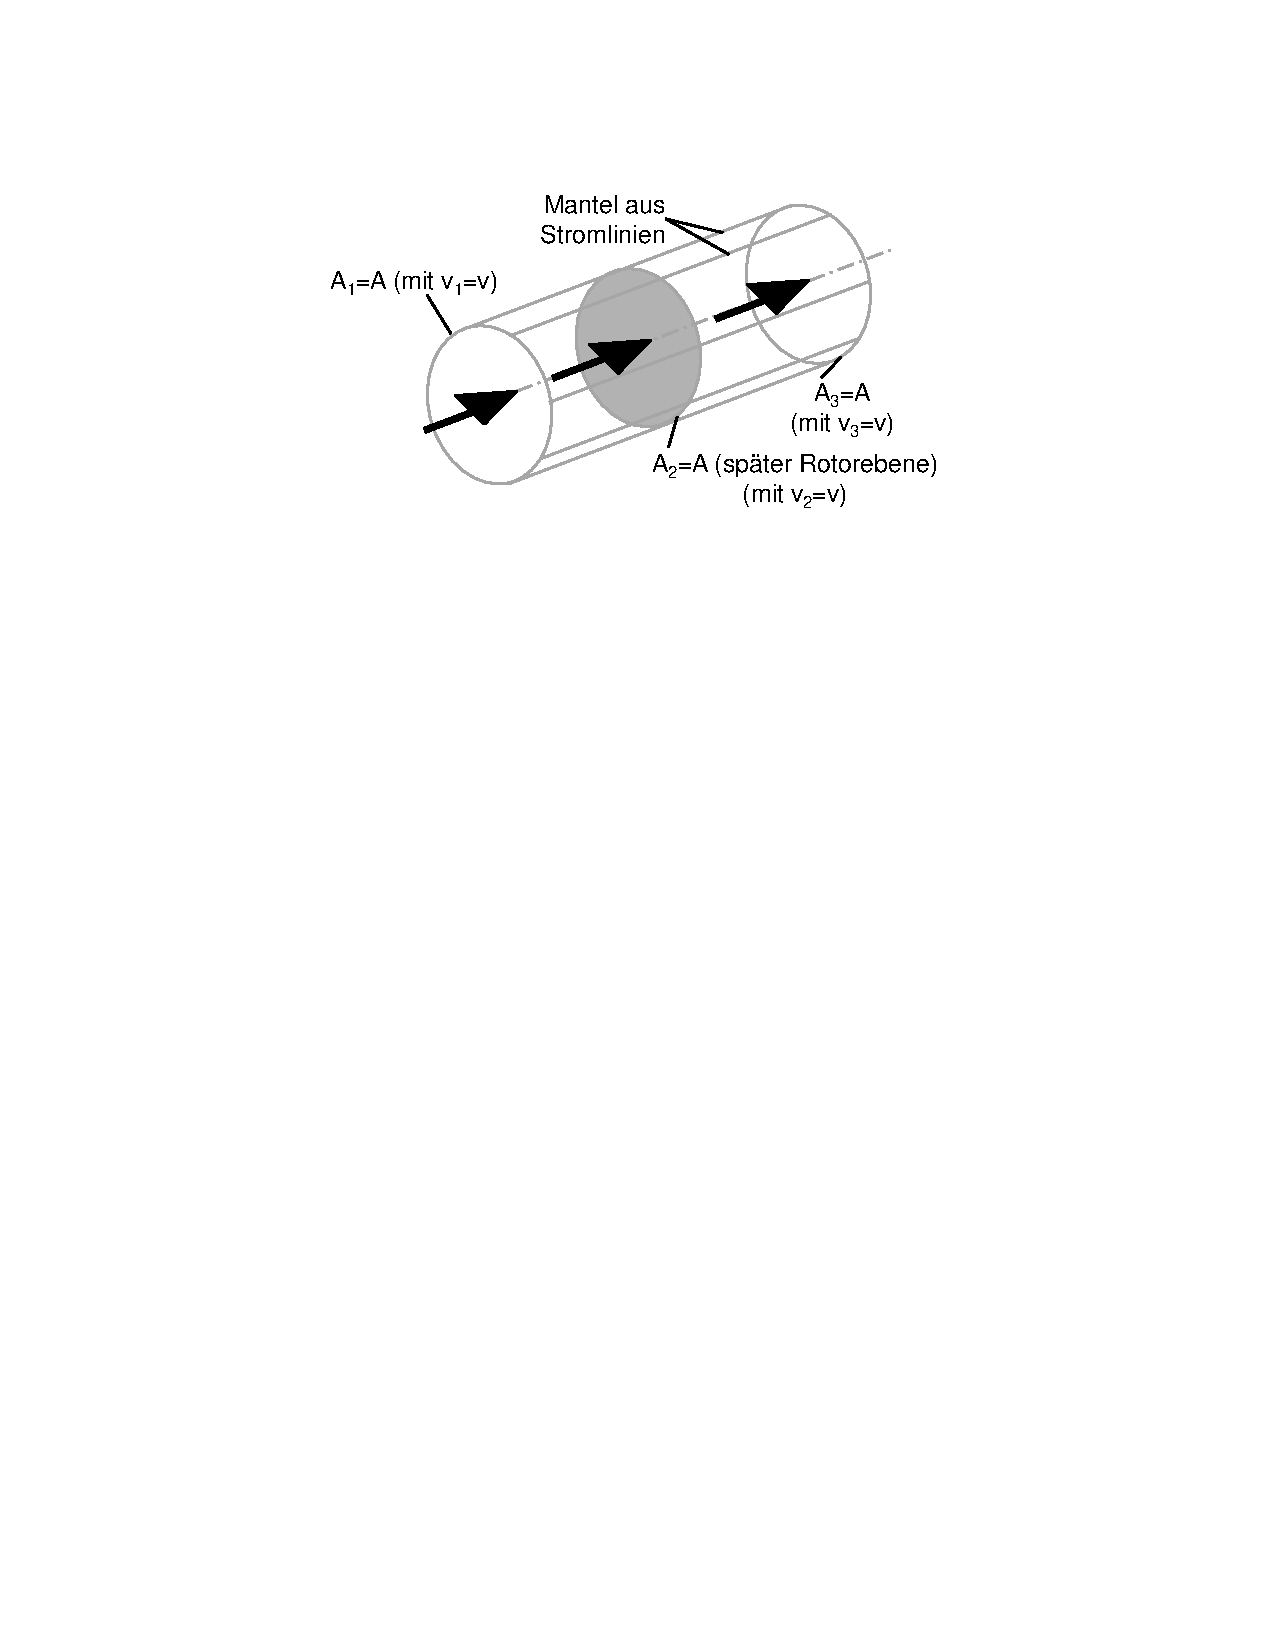
\includegraphics[width=0.5\textwidth]{Bilder/Kapitel 2/ungestörte_stromröhre.pdf}}
   \caption[Ungestörte Luftröhre]{Ungestörte Luftröhre \cite{SkriptSchulte}}
   \label{fig:Bild2.1}
\end{figure}

Folgende weitere Annahmen werden getroffen:
\begin{itemize}
    \item konstante Querschnittsflächen: $\acs{Ai} = const.$
    \item stationäre gleichförmige Strömung: $\acs{vi}(t_{\mathrm{1}}) = \acs{vi}(t_{\mathrm{2}}) = \acs{vi} = const.$
    \item geringe Druckunterschiede: $\acs{rhoi} = const.$
    \item Index i = 1; 2; 3
\end{itemize}
\bigskip
Der ungestörte Luftmassenstrom folgt zu: 
\begin{equation} \label{eq:Gleichung2.1}
    \boxed{\acs{mdoti} = \acs{rhoi} \cdot \acs{vi} \cdot \acs{Ai} = const.}
\end{equation}

\paragraph{Windleistung \acs{PW}}\mbox{}\smallskip\\
Zur Berechnung der Windleistung \acs{PW} wird der ungestörte Luftmassenstrom (\autoref{eq:Gleichung2.1}) mit der Annahme, dass die Querschnittsflächen aus dem Rotoraußenradius \acs{R} berechnet werden (\autoref{eq:Gleichung2.2}), verwendet.
\begin{align}
    \acs{Ai} = \acs{pi}\cdot \acs{R}^2
    \label{eq:Gleichung2.2}
\end{align}
\newline
Die Windleistung folgt aus der zeitlichen Differentiation der kinetischen Windenergie \acs{EW} nach der Luftmasse \acs{m} und der Windgeschwindigkeit \acs{v}. 
\begin{align}
    \acs{EW} &= \frac{1}{2} \cdot \acs{mi} \cdot \acs{vi}^2 \nonumber \\
    \acs{PW} &= \frac{d}{dt}(\acs{EW}) \label{eq:Gleichung2.3} \\
    \acs{PW} &= \frac{1}{2} \cdot \acs{mdoti} \cdot \acs{vi}^2 + \frac{1}{2} \cdot \acs{mi} \cdot 2 \cdot \acs{vdoti}^2 \label{eq:Gleichung2.4}
\end{align}
\newline
Da eine stationäre Strömung vorliegt, ist die Änderung der Windgeschwindigkeit gleich Null ($\acs{vdoti} = 0$). Folglich wird die \autoref{eq:Gleichung2.4} vereinfacht.
\begin{align}
    \acs{PW} &= \frac{1}{2} \cdot \acs{mdoti} \cdot \acs{vi}^2 \label{eq:Gleichung2.5}
\end{align}
\newline
Durch das Einsetzen des ungestörten Luftmassenstromes aus \autoref{eq:Gleichung2.1} in die \autoref{eq:Gleichung2.5} resultiert die mathematische Formel zur Berechnung der zugefügten Windleistung \acs{PW}. Die Windgeschwindigkeit \acs{v1} und die Zwischenfläche \acs{A2} sind entscheidend. Die Luftdichte \acs{rho} wird wie o.g. als konstant angenommen.
\begin{align*}
    \acs{PW} &= \frac{1}{2} \cdot \acs{rho} \cdot \acs{v1} \cdot \acs{A2} \cdot \acs{v1}^2
\end{align*}
\begin{equation}\label{eq:Gleichung2.6}
    \boxed{\acs{PW} = \frac{1}{2} \cdot \acs{rho} \cdot \acs{A2} \cdot \acs{v1}^3} 
\end{equation}

\paragraph{Staukraft \acs{FST}}\mbox{}\smallskip\\
Zur Vorbereitung auf die Tragflügeltheorie wird die Formel zur Berechnung der Windleistung zu einem Produkt aus Staukraft \acs{FST} und ungestörter Windgeschwindigkeit \acs{v1} vereinfacht. Die Staukraft resultiert aus dem Produkt von Staudruck \acs{pST} und der Querschnittsfläche \acs{A2}.
\begin{align*}
    \acs{pST} = \frac{1}{2} \cdot \acs{rho} \cdot \acs{v1}^2 \\
    \acs{FST} = \acs{pST} \cdot \acs{A2}
\end{align*}
\begin{equation} \label{eq:Gleichung2.7}
    \boxed{\acs{PW} = \acs{FST} \cdot \acs{v1}}
\end{equation}

\subsubsection{Gestörter Luftmassenstrom}

\paragraph{Adaptierung des ungestörten Stromröhrenmodells}\mbox{}\smallskip\\
In der Realität liegt zwischen der Ein- und Austrittsfläche der Stromröhre ein Objekt (z.B. ein WEA-Rotor), welcher ein Strömungshindernis darstellt und den Luftmassenstrom verzögert (\autoref{fig:Bild2.2}). Die Verzögerung hat einen Abfall der Windgeschwindigkeiten $\acs{v2}$ und $\acs{v3}$ zur Folge.
\begin{align*}
    \acs{v1} > \acs{v2} > \acs{v3}
\end{align*}
\newline
Wird der ungestörte Luftmassenstrom mit gleichbleibender Windgeschwindigkeit $\acs{v2}$ und Querschnittfläche $\acs{A2}$ vorausgesetzt, muss die Querschnittsfläche $\acs{A1}$ verjüngt und die Fläche $\acs{A3}$ vergrößert werden, sodass weiterhin \autoref{eq:Gleichung2.1} gilt.
\begin{align*}
    \acs{A1} < \acs{A2} < \acs{A3}
\end{align*}
\begin{figure}[H]
   \centering
   \fbox{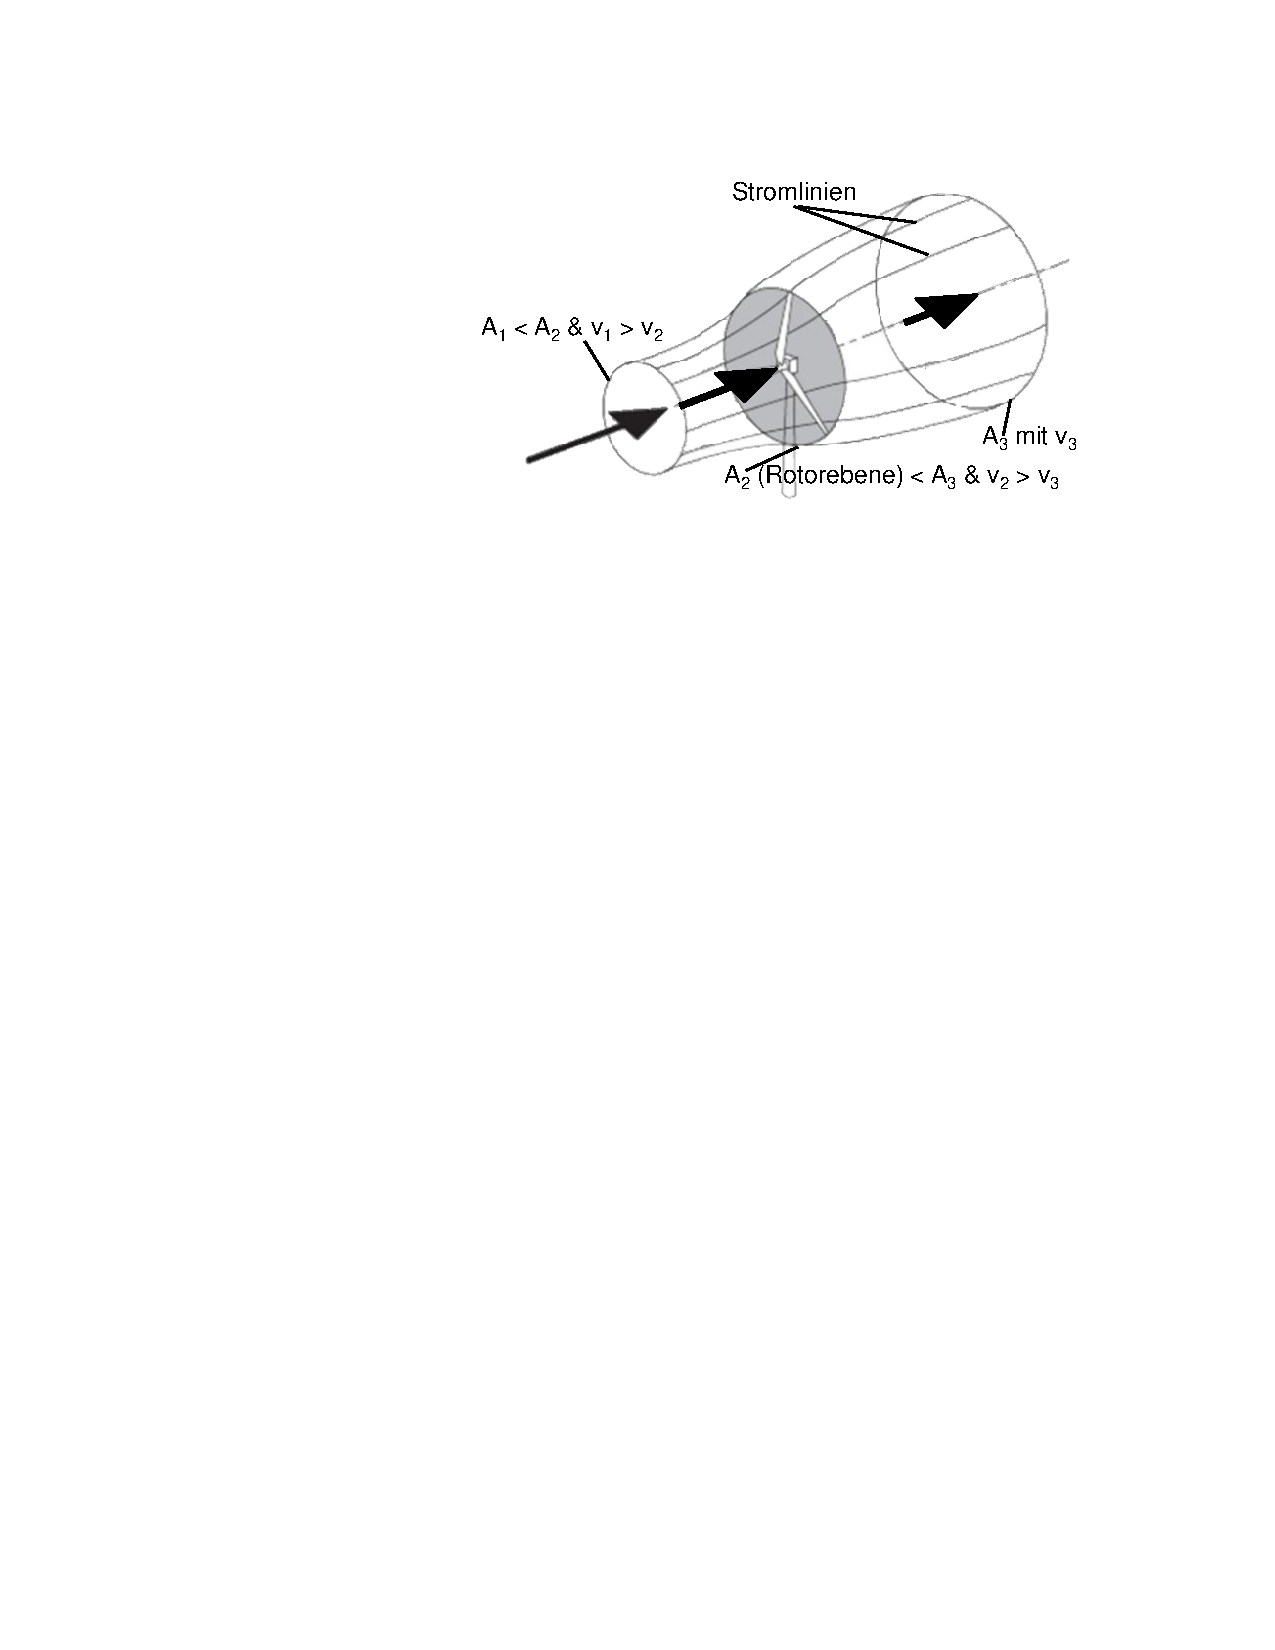
\includegraphics[width=0.5\textwidth]{Bilder/Kapitel 2/gestörte_stromröhre.pdf}}
   \caption[Gestörte Luftröhre]{Gestörte Luftröhre \cite{SkriptSchulte}}
   \label{fig:Bild2.2}
\end{figure}

\paragraph{Drehzahlunabhängige Rotorleistung \acs{PR}}\mbox{}\smallskip\\
Die direkte Messung der Windgeschwindigkeit $\acs{v2}$ am Rotorblatt ist kaum möglich. Somit wird im ersten Ansatz die Rotorleistung $\acs{PR}$ mithilfe der \autoref{eq:Gleichung2.5} aus der Differenz der Windleistung vor dem Rotor und nach dem Rotor berechnet.
\begin{align*} \label{eq:Gleichung2.8}
    \acs{PR} = \acs{PW}(\acs{v1}) - \acs{PW}(\acs{v3})
\end{align*}
\begin{equation}\label{eq:Gleichung2.8}
    \boxed{\acs{PR} = \frac{1}{2} \cdot \acs{mdoti} \cdot (\acs{v1}^2 - \acs{v3}^2)}
\end{equation}

\paragraph{Einfluss der Rotordrehzahl \acs{nR}}\mbox{}\smallskip\\
Die entnommene Rotorleistung ist abhängig von der Windgeschwindigkeit $\acs{v2}$, der Rotordrehzahl \acs{nR} und aerodynamischen Effekten. Um die maximal mögliche Leistung für unterschiedliche Arbeitspunkte zu bestimmen, werden WEA-Kennfelder aufgenommen, welche im späteren Verlauf weiter definiert werden. Für eine erste Betrachtung über die Lage des Maximums werden zwei extreme Betriebspunkte festgelegt:
\begin{itemize}
    \item Rotorstillstand: $\acs{nR}$ = 0 $\rightarrow$ kaum Verzögerung
    \item Verblockung: $\acs{nR}$ >> 0 $\rightarrow$ nahezu Verstopfung
\end{itemize}

In beiden Fällen ist die entnommene Rotorleistung annähernd Null. Aus den Grenzfällen wird geschlussfolgert, dass das Maximum der Rotorleistung zwischen diesen Punkten liegen muss.\\
Aus dem Froude-Rankineschen Theorem geht hervor, dass die Windgeschwindigkeit des Rotors $\acs{v2}$ den Mittelwert der ungestörten Windgeschwindigkeit $\acs{v1}$ und der reduzierten Windgeschwindigkeit $\acs{v3}$ darstellt. Somit gilt:
\begin{equation}\label{eq:Gleichung2.9}
    \boxed{\acs{v2} = \frac{\acs{v1} + \acs{v3}}{2}}
\end{equation}
\newline
Der resultierende Luftmassenstrom gemäß \autoref{eq:Gleichung2.5} folgt zu:
\begin{align*}
    \acs{mdot} = \acs{rho} \cdot \acs{v2} \cdot \acs{A2}
\end{align*}
\begin{equation}\label{eq:Gleichung2.10}
    \boxed{\acs{mdot} = \acs{rho} \cdot \frac{\acs{v1} + \acs{v3}}{2} \cdot \acs{A2}}
\end{equation}
\newline
Durch das Einsetzen der Zusammenhänge aus \autoref{eq:Gleichung2.8} in \autoref{eq:Gleichung2.10} folgt die Gleichung zur Berechnung der Rotorleistung $\acs{PR}$ in Abhängigkeit der Rotordrehzahl $\acs{nR}$.
\begin{align*}
    \acs{PR} &= \frac{1}{2} \cdot \acs{rho} \cdot \frac{\acs{v1} + \acs{v3}}{2} \cdot \acs{A2} \cdot (\acs{v1}^2 - \acs{v3}^2) \\
    \acs{PR} &= \frac{1}{2} \cdot \acs{rho} \cdot \acs{A2} \cdot \frac{1}{2} \cdot \acs{v1} \cdot (1 + \frac{\acs{v3}}{\acs{v1}}) \cdot \acs{v1}^2 \cdot (1 - \frac{\acs{v3}^2}{\acs{v1}^2})
\end{align*}
\newline
Wird nun der Term $(\frac{1}{2} \cdot \acs{rho} \cdot \acs{v1} \cdot \acs{A2} \cdot \acs{v1}^2)$ durch $\acs{PW}$ aus \autoref{eq:Gleichung2.6} ersetzt, resultiert:
\begin{equation}\label{eq:Gleichung2.11}
    \boxed{\acs{PR} = \acs{PW} \cdot \frac{1}{2} \cdot (1 + \frac{\acs{v3}}{\acs{v1}}) \cdot (1 - \frac{\acs{v3}^2}{\acs{v1}^2})}
\end{equation}

\paragraph{Leistungsbeiwert \acs{cP}}\mbox{}\smallskip\\
Die \autoref{eq:Gleichung2.11} wird weiter zu einem Produkt aus der Windleistung $\acs{PW}$ und einem dimensionslosen Leistungsbeiwert $\acs{cP}$ zusammengefasst. Der Leistungsbeiwert nimmt nur Werte zwischen Null und Eins an und beschreibt das Verhältnis von entnommener Rotorleistung $\acs{PR}$ zu zugefügter Windleistung $\acs{PW}$.
\begin{align*}
    \acs{cP} = \frac{1}{2} \cdot (1 + \frac{\acs{v3}}{\acs{v1}}) \cdot (1 - \frac{\acs{v3}^2}{\acs{v1}^2})
\end{align*}
\begin{equation}\label{eq:Gleichung2.12}
    \boxed{\acs{PR} = \acs{PW} \cdot \acs{cP}}
\end{equation}
\begin{equation}\label{eq:Gleichung2.13}
    \boxed{\acs{cP} = \frac{\acs{PR}}{\acs{PW}}}
\end{equation}
\newline
Ist der Leistungsbeiwert gleich Eins, entnimmt die WEA 100\% der Windleistung. Dies ist in der Realität u.a. aufgrund von aerodynamischen Effekten nicht möglich. Bei einer optimalen Verzögerung wird ein Wert von ca. 59\% ($\frac{16}{27}$) erreicht, welcher als Betzscher Leistungsbeiwert ($\acs{cPmax}$) bezeichnet wird. Dieser Wert wird ausschließlich bei folgender Konstellation ausgehend von der Windgeschwindigkeit $\acs{v1}$ erreicht. Diese Annahme ist jedoch hypothetisch, d.h. in Realität liegt der maximale Leistungsbeiwert bei ca. 45 bis 48\%.
\begin{itemize}
    \item $\acs{v2} = \frac{2}{3} \cdot \acs{v1}$
    \item $\acs{v3} = \frac{1}{3} \cdot \acs{v1}$
\end{itemize}
Weichen die Windgeschwindigkeiten am Rotor und hinter der WEA von den o.g. Faktoren ab, ist das Verhältnis von entnommener zu zugefügter Leistung geringer als der Betzsche Leistungsbeiwert.

\subsection{Tragflügeltheorie}

\subsubsection{Auftrieb und Widerstand eines Tragflügels}
Wird ein Tragflügel von einem Wind der Geschwindigkeit $\acs{v}$ erfasst, entsteht eine resultierende Geschwindigkeit $\acs{c}$ (Anströmgeschwindigkeit) (\autoref{fig:Bild2.3}), welche über die Wurzel der quadratischen Summe aus Windgeschwindigkeit $\acs{v}$ und der relativen Bewegungsgeschwindigkeit $\acs{u'}$ berechnet wird (\autoref{eq:Gleichung2.14}). Die relative Bewegungsgeschwindigkeit \acs{u'} folgt aus der Negation der quer zur Windgeschwindigkeit stehenden Bewegungsgeschwindigkeit \acs{u}.
\begin{align} \label{eq:Gleichung2.14}
    \acs{c} = \sqrt{\acs{v}^2 + (\acs{u'})^2}
\end{align}
\begin{figure}[H]
   \centering
   \fbox{\includegraphics[width=0.34\textwidth]{Bilder/Kapitel 2/auftrieb_widerstand_tragflügel.pdf}}
   \caption[Anströmverhältnisse eines Tragflügels]{Anströmverhältnisse eines Tragflügels \cite{SkriptSchulte}}
   \label{fig:Bild2.3}
\end{figure}

Die Anströmgeschwindigkeit ist über die Tragflügellänge konstant. Durch die Luftanströmung werden Luftpartikel an der oberen Tragflügelseite beschleunigt und an der unteren Tragflügelseite abgebremst. Dadurch entstehen eine Saugseite (beschleunigte Luftpartikel) und eine Druckseite (gebremste Luftpartikel). Die unterschiedlichen Strömungsgeschwindigkeiten führen zu einem Druckunterschied zwischen der oberen und unteren Tragflügelseite. Der Überdruck unter dem Tragflügel führt zu einer Auftriebskraft \acs{FA}, wohingegen der Unterdruck auf der Oberseite eine Widerstandkraft \acs{FW} hervorruft (\autoref{fig:Bild2.4}).
\begin{figure}[H]
   \centering
   \fbox{\includegraphics[width=0.39\textwidth]{Bilder/Kapitel 2/druckverhältnisse.pdf}}
   \caption[Saug- und Druckseite]{Saug- und Druckseite \cite{SkriptSchulte}}
   \label{fig:Bild2.4}
\end{figure}
\newpage
\paragraph{Auftriebskraft \acs{FA} und Widerstandskraft \acs{FW}}\mbox{}\smallskip\\
Durch die Abgrenzung von Saug- und Druckseite durch eine Profilsehne entsteht ein Anstellwinkel \acs{alpha} zwischen der Profilsehne und des Vektors der Anströmgeschwindigkeit \acs{c}. Die Widerstandkraft verläuft in Richtung der Anströmgeschwindigkeit, wohingegen die Auftriebskraft senkrecht zu dieser steht (\autoref{fig:Bild2.5}). Aus den Kenntnissen über die Tiefe \acs{tflug} und Breite \acs{bflug} eines Tragflügels werden die Auftriebs- und Widerstandkraft nach \autoref{eq:Gleichung2.15} und \autoref{eq:Gleichung2.16} berechnet.
\begin{align}
    \acs{FA} = \acs{cA}(\acs{alpha}) \cdot \frac{1}{2} \cdot \acs{rho} \cdot \acs{c}^2 \cdot (\acs{tflug} \cdot \acs{bflug}) \label{eq:Gleichung2.15} \\
    \acs{FW} = \acs{cW}(\acs{alpha}) \cdot \frac{1}{2} \cdot \acs{rho} \cdot \acs{c}^2 \cdot (\acs{tflug} \cdot \acs{bflug}) \label{eq:Gleichung2.16}
\end{align}
\begin{figure}[H]
   \centering
   \fbox{\includegraphics[width=0.6\textwidth]{Bilder/Kapitel 2/kräfte.pdf}}
   \caption[Auftriebs- und Widerstandskraft]{Auftriebs- und Widerstandskraft \cite{SkriptSchulte}}
   \label{fig:Bild2.5}
\end{figure}

\paragraph{Auftriebsbeiwert \acs{cA} und Widerstandsbeiwert \acs{cW}}\mbox{}\smallskip\\
Die Faktoren \acs{cA} und \acs{cW} stellen den Auftriebs- und Widerstandsbeiwert dar und hängen vom Anstellwinkel \acs{alpha} ab. Die jeweiligen Werte werden messtechnisch ermittelt und sind für jede Tragflügelkontur unterschiedlich (\autoref{fig:Bild2.6}).
\begin{figure}[H]
   \centering
   \fbox{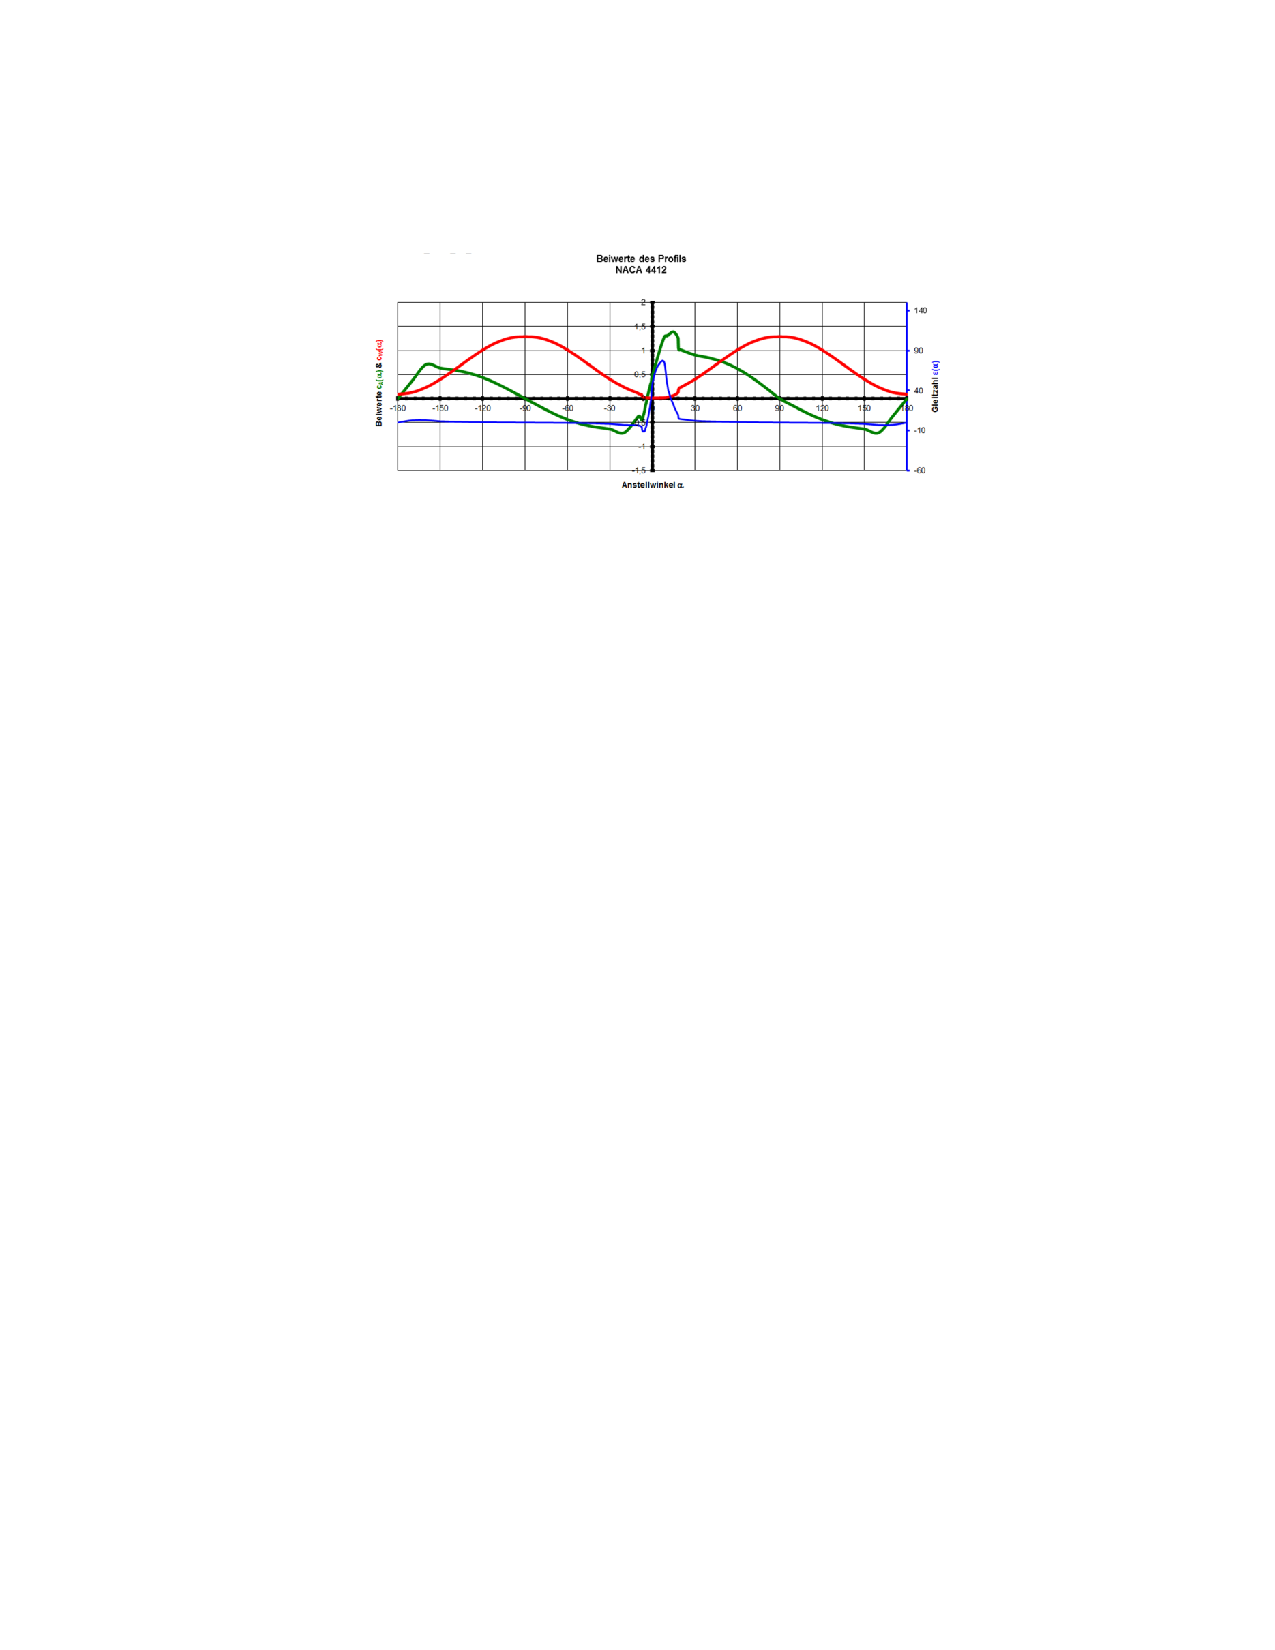
\includegraphics[width=0.5\textwidth]{Bilder/Kapitel 2/beiwerte.pdf}}
   \caption[Beispielverlauf der Beiwerte]{Beispielverlauf der Beiwerte \cite{SkriptSchulte}}
   \label{fig:Bild2.6}
\end{figure}
\newpage
Wird der Quotient aus Antriebskraft \acs{FA} und Widerstandskraft \acs{FW} gebildet, folgt die Gleitzahl \acs{eps}. Diese Verhältnis wird optimal, wenn im Verhältnis zum Widerstand ein maximaler Auftrieb erzeugt wird. Daraus resultiert ein optimaler Anstellwinkel \acs{alphaopt}.
\begin{align}
    \frac{\acs{FA}}{\acs{FW}} &= \frac{\acs{cA}(\acs{alpha}) \cdot \frac{1}{2} \cdot \acs{rho} \cdot \acs{c}^2 \cdot (\acs{tflug} \cdot \acs{bflug})}{\acs{cW}(\acs{alpha}) \cdot \frac{1}{2} \cdot \acs{rho} \cdot \acs{c}^2 \cdot (\acs{tflug} \cdot \acs{bflug})} \nonumber \\
    \frac{\acs{FA}}{\acs{FW}} &= \frac{\acs{cA}(\alpha)}{\acs{cW}(\alpha)} \label{eq:Gleichung2.17}
\end{align}
\begin{equation} \label{eq:Gleichung2.18}
    \boxed{\acs{eps}(\acs{alpha}) = \frac{\acs{FA}}{\acs{FW}}}
\end{equation}
\newline
Wird ein blattprofilspezifischer Wert des Anstellwinkels überschritten, folgt ein Strömungsabriss, d.h. die Luftpartikel folgen nicht länger der Tragflügelkontur.

\subsubsection{Anströmverhältnisse am Rotorblatt}

\paragraph{Anströmungs- und Umfangsgeschwindigkeit}\mbox{}\smallskip\\
Basierend auf \autoref{eq:Gleichung2.14} wird die Anströmungsgeschwindigkeit $\acs{c}\left(\acs{R}, \acs{nR}\right)$ aus der Wurzel der quadratischen Summe von der Windgeschwindigkeit \acs{v2} in der Rotorebene und der Umfangsgeschwindigkeit $\acs{u}\left(\acs{R}, \acs{nR}\right)$ infolge der Rotordrehung berechnet (\autoref{eq:Gleichung2.19}) (\autoref{fig:Bild2.7}).
\begin{equation} \label{eq:Gleichung2.19}
    \boxed{\acs{c}\left(\acs{R}, \acs{nR}\right) = \sqrt{\acs{v2}^2 + \acs{u}(\acs{R}, \acs{nR})^2}}
\end{equation}
\begin{figure}[H]
   \centering
   \fbox{\includegraphics[width=0.6\textwidth]{Bilder/Kapitel 2/anströmungs_umfangsgeschwindigkeit.pdf}}
   \caption[Antrömverhältnisse eines Rotorblattes]{Anströmverhältnisse eines Rotorblattes \cite{SkriptSchulte}}
   \label{fig:Bild2.7}
\end{figure}

Die Umfangsgeschwindigkeit \acs{u} des Rotors ist abhängig von der Rotordrehzahl \acs{nR} und dem Rotoraußenradius \acs{R} (\autoref{eq:Gleichung2.20}). Mit steigendem Radius zur Blattspitze nimmt die Umfangsgeschwindigkeit und somit auch die Anströmgeschwindigkeit zu.
\begin{equation} \label{eq:Gleichung2.20}
    \boxed{\acs{u}(\acs{R}, \acs{nR}) = \acs{omegaR} \cdot \acs{R} = 2 \cdot \acs{pi} \cdot \acs{nR} \cdot \acs{R}}
\end{equation}

\paragraph{Schnelllaufzahl \acs{lambda}}\mbox{}\smallskip\\
Zur aerodynamischen Auslegung der Rotorblätter ist die Kenntnis über das Verhältnis von Blattspitzengeschwindigkeit $\acs{u}\left(\acs{R}, \acs{nR}\right)$ zur ungestörten Windgeschwindigkeit \acs{v1} wichtig. Dieses Verhältnis wird als Schnelllaufzahl \acs{lambda} deklariert.
\begin{equation} \label{eq:Gleichung2.21}
    \boxed{\acs{lambda}\left(\acs{R}, \acs{nR}\right) = \frac{\acs{u}\left(\acs{R}, \acs{nR}\right)}{\acs{v1}} = \frac{\acs{omegaR}\left(\acs{nR}\right) \cdot \acs{R}}{\acs{v1}}}
\end{equation}

\paragraph{Anstellwinkel \acs{alpha} und Anströmwinkel \acs{gamma}}\mbox{}\smallskip\\
Der Anstellwinkel $\acs{alpha}\left(\acs{R}\right)$ hängt vom Tragflügelprofil ab und repräsentiert den Winkel zwischen der Anströmgeschwindigkeit $\acs{c}\left(\acs{R}, \acs{nR}\right)$ und der Profilsehne, welche die Trennlinie zwischen der Druck- und Saugseite darstellt (\autoref{fig:Bild2.8}).
\begin{figure}[H]
   \centering
   \fbox{\includegraphics[width=0.6\textwidth]{Bilder/Kapitel 2/anstell_anströmwinkel.pdf}}
   \caption[Anstell- und Anströmwinkel]{Anstell- und Anströmwinkel \cite{SkriptSchulte}}
   \label{fig:Bild2.8}
\end{figure}

Der Anströmwinkel $\acs{gamma}\left(\acs{R}, \acs{nR}\right)$ hängt von der Windgeschwindigkeit \acs{v2} und der Umfangsgeschwindigkeit $\acs{u}\left(\acs{R}, \acs{nR}\right)$ ab. Sind beide Größen bekannt, resultiert der Anströmwinkel aus folgender \autoref{eq:Gleichung2.22}.
\begin{equation} \label{eq:Gleichung2.22}
	\boxed{\acs{gamma}\left(\acs{R}, \acs{nR}\right) = \arctan\left(\frac{\acs{v2}}{\acs{u}\left(\acs{R}, \acs{nR}\right)}\right)}
\end{equation}
\newline
Die eben aufgeführte Gleichung hängt ebenso wie die Anströmgeschwindigkeit \acs{c} nur von der Windgeschwindigkeit \acs{v2} in der Rotorebene und der Umfangsgeschwindigkeit $\acs{u}\left(\acs{R}, \acs{nR}\right)$ ab. Somit hängt die Anströmgeschwindigkeit \acs{gamma} direkt vom Anströmwinkel \acs{alpha} ab. Es gilt:
\begin{equation} \label{eq:Gleichung2.23}
	\boxed{\acs{c}\left(\acs{R}, \acs{nR}\right) = \acs{c}\left(\acs{gamma}(\acs{R}, \acs{nR})\right)}
\end{equation}

\paragraph{Bauwinkel \acs{beta}}\mbox{}\smallskip\\
Der Bauwinkel $\acs{beta}\left(\acs{R}, \acs{nR}\right)$ wird beim Entwurf eines neuen Rotorblattes festgelegt und liegt zwischen der Rotorebene und der Profilsehne (\autoref{fig:Bild2.9}). Auf Grundlage dessen resultiert ein optimales Anströmverhältnis aus Antriebskraft $\acs{FA}\left(\acs{alpha}\left(\acs{R}, \acs{nR}\right)\right)$ zu Widerstandskraft $\acs{FW}\left(\acs{alpha}\left(\acs{R}, \acs{nR}\right)\right)$. Der Anstellwinkel $\acs{alpha}\left(\acs{R}, \acs{nR}\right)$ liegt genau im Optimum $\acs{alphaopt}\left(\acs{R}, \acs{nR}\right)$. Durch den Einbauwinkel kann der Anströmwinkel $\acs{gamma}\left(\acs{R}, \acs{nR}\right)$ aus der Summe von Anstellwinkel $\acs{alpha}\left(\acs{R}, \acs{nR}\right)$ und Bauwinkel $\acs{beta}\left(\acs{R}, \acs{nR}\right)$ berechnet werden (\autoref{eq:Gleichung2.24}).
\begin{align} \label{eq:Gleichung2.24}
	\acs{gamma}\left(\acs{R}, \acs{nR}\right) = \acs{alpha}\left(\acs{R}, \acs{nR}\right) + \acs{beta}\left(\acs{R}, \acs{nR}\right)
\end{align}
\begin{figure}[H]
   \centering
   \fbox{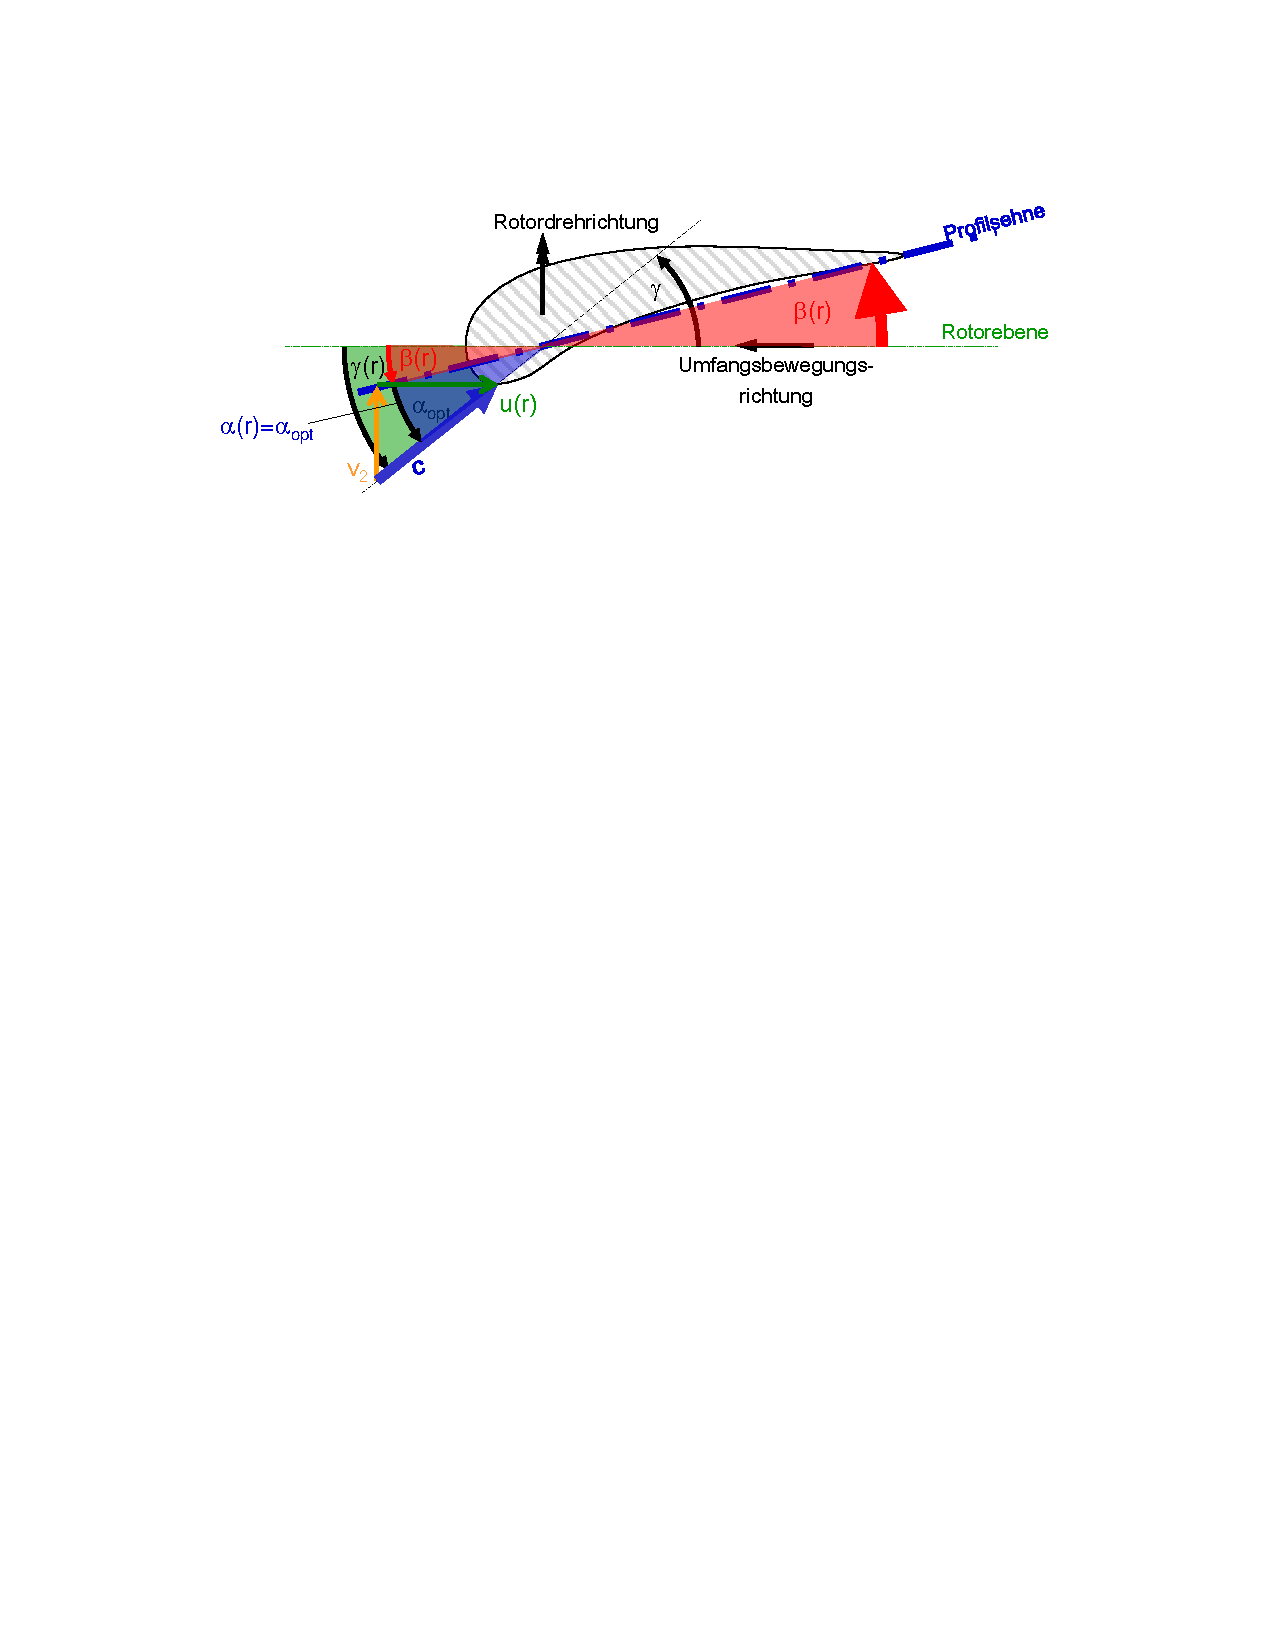
\includegraphics[width=0.6\textwidth]{Bilder/Kapitel 2/bauwinkel.pdf}}
   \caption[Bauwinkel]{Bauwinkel \cite{SkriptSchulte}}
   \label{fig:Bild2.9}
\end{figure}

Da die Umfangsgeschwindigkeit bei gleichbleibenden Windverhältnissen von der Blattspitze bis zur Blattwurzel linear abnimmt und trotzdem ein optimale Anstellwinkel über die gesamte Blattlänge erreicht werden soll, muss das Rotorblatt verwunden werden. Andernfalls würde das Anströmverhältnis nicht im Optimum liegen. Der Bauwinkel nimmt zur Blattspitze hin ab. Die Blattkontur kann während des Betriebs nicht weiter verändert werden, folglich kann der Anstellwinkel nur noch durch die Anpassung der Rotordrehzahl, als auch durch das Verdrehen des gesamten Rotorblattes (Pitchen) verändert werden.

\paragraph{Wirkung der Auftriebs- und Widerstandskraft}\mbox{}\smallskip\\
Die Gleichungen zur Berechnung der Auftriebs- und Widerstandkraft beruhen auf \autoref{eq:Gleichung2.15} und \autoref{eq:Gleichung2.16}. Da die Anströmgeschwindigkeit $\acs{c}\left(\acs{R}, \acs{nR}\right)$ ebenfalls vom Anströmwinkel $\acs{gamma}\left(\acs{R}, \acs{nR}\right)$ abhängt, folgt:
\begin{align}
    \acs{FA}\left(\acs{alpha}\left(\acs{R}, \acs{nR}\right), \acs{gamma}\left(\acs{R}, \acs{nR}\right)\right) &= \acs{cA}\left(\acs{alpha}\left(\acs{R}, \acs{nR}\right)\right) \cdot \frac{1}{2} \cdot \acs{rho} \cdot \acs{c}\left(\acs{gamma}\left(\acs{R}, \acs{nR}\right)\right)^2 \cdot  \left(\acs{tflug} \cdot \acs{bflug}\right) \label{eq:Gleichung2.25} \\
    \acs{FW}\left(\acs{alpha}\left(\acs{R}, \acs{nR}\right), \acs{gamma}\left(\acs{R}, \acs{nR}\right)\right) &= \acs{cW}\left(\acs{alpha}\left(\acs{R}, \acs{nR}\right)\right) \cdot \frac{1}{2} \cdot \acs{rho} \cdot \acs{c}\left(\acs{gamma}\left(\acs{R}, \acs{nR}\right)\right)^2 \cdot \left(\acs{tflug} \cdot \acs{bflug}\right) \label{eq:Gleichung2.26}
\end{align}
Aus der Wurzel der quadratischen Addition von Auftriebs- und Widerstandskraft folgt eine resultierende Gesamtkraft $\acs{Fres}\left(\acs{alpha}, \acs{gamma}\right)$ (\autoref{eq:Gleichung2.27}), welche aus einer resultierenden Umfangskraft $\acs{deltaFU}\left(\acs{alpha}, \acs{gamma}\right)$ und einer Schubkraft $\acs{deltaFS}\left(\acs{alpha}, \acs{gamma}\right)$ besteht (\autoref{fig:Bild2.10}). Die resultierende Umfangskraft hat Biege- und Schubbelastungen von den Rotorblättern, Gondel, Turm und des Fundaments zur Folge. Hingegen erzeugt die Schubkaft eine Beschleunigung und Verzögerung der Rotordrehung.
\begin{equation}\label{eq:Gleichung2.27}
    \boxed{\acs{Fres}\left(\acs{alpha}, \acs{gamma}\right) = \sqrt{\acs{FA}\left(\acs{alpha}, \acs{gamma}\right)^2 + \acs{FW}\left(\acs{alpha}, \acs{gamma}\right)^2}}
\end{equation}
\begin{figure}[H]
   \centering
   \fbox{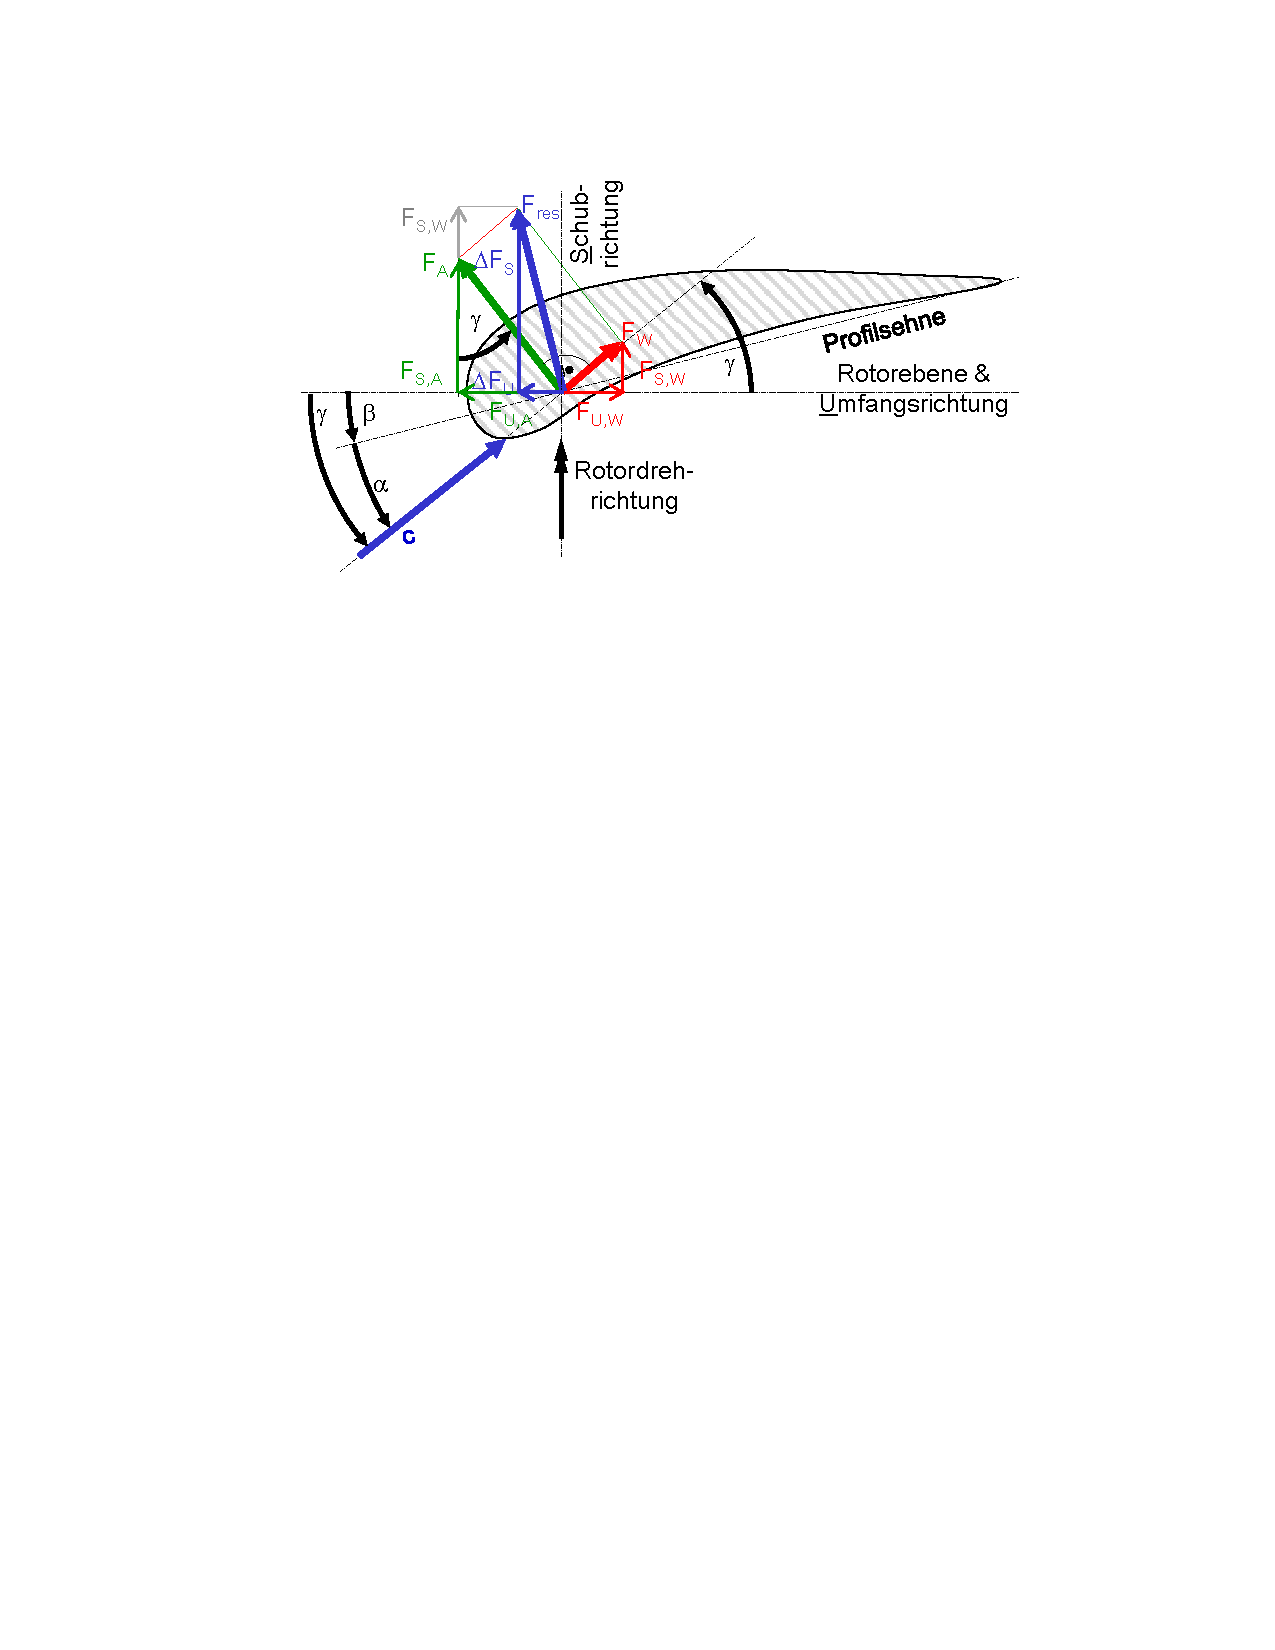
\includegraphics[width=0.6\textwidth]{Bilder/Kapitel 2/wirkung_auftriebs_widerstandskraft.pdf}}
   \caption[Wirkung der Auftriebs- und Widerstandskraft]{Wirkung der Auftriebs- und Widerstandskraft \cite{SkriptSchulte}}
   \label{fig:Bild2.10}
\end{figure}

Die Kräfte $\acs{deltaFU}\left(\acs{alpha}, \acs{gamma}\right)$ und $\acs{deltaFS}\left(\acs{alpha}, \acs{gamma}\right)$ können aus den Längs- und Querkräften der Antriebs- und Widerstandskräften berechnet werden.
\begin{align*}
    \acs{FUA}\left(\acs{alpha}, \acs{gamma}\right) &= \acs{FA}\left(\acs{alpha}, \acs{gamma}\right) \cdot \sin(\acs{gamma}\left(\acs{R}, \acs{nR}\right))\\
    \acs{FUW}\left(\acs{alpha}, \acs{gamma}\right) &= \acs{FW}\left(\acs{alpha}, \acs{gamma}\right)\cdot \cos(\acs{gamma}\left(\acs{R}, \acs{nR}\right)) \\ 
    \acs{deltaFU}\left(\acs{alpha}, \acs{gamma}\right) &= \acs{FUA}\left(\acs{alpha}, \acs{gamma}\right) - \acs{FUW}\left(\acs{alpha}, \acs{gamma}\right)
\end{align*}
\begin{equation} \label{eq:Gleichung2.28}
    \boxed{\acs{deltaFU}\left(\acs{alpha}, \acs{gamma}\right) = \acs{FA}\left(\acs{alpha}, \acs{gamma}\right) \cdot \sin(\acs{gamma}\left(\acs{R}, \acs{nR}\right)) - \acs{FW}\left(\acs{alpha}, \acs{gamma}\right) \cdot \cos(\acs{gamma}\left(\acs{R}, \acs{nR}\right))}
\end{equation}
\smallskip
\begin{align*}
    \acs{FSA}\left(\acs{alpha}, \acs{gamma}\right) &= \acs{FA}\left(\acs{alpha}, \acs{gamma}\right) \cdot \cos(\acs{gamma}\left(\acs{R}, \acs{nR}\right))\\
    \acs{FSW}\left(\acs{alpha}, \acs{gamma}\right) &= \acs{FW}\left(\acs{alpha}, \acs{gamma}\right) \cdot \sin(\acs{gamma}\left(\acs{R}, \acs{nR}\right)) \\ 
    \acs{deltaFS}\left(\acs{alpha}, \acs{gamma}\right) &= \acs{FSA}\left(\acs{alpha}, \acs{gamma}\right) + \acs{FSW}\left(\acs{alpha}, \acs{gamma}\right)
\end{align*}
\begin{equation} \label{eq:Gleichung2.29}
    \boxed{\acs{deltaFS}\left(\acs{alpha}, \acs{gamma}\right) = \acs{FA}\left(\acs{alpha}, \acs{gamma}\right) \cdot \cos(\acs{gamma}\left(\acs{R}, \acs{nR}\right)) - \acs{FW}\left(\acs{alpha}, \acs{gamma}\right) \cdot \sin(\acs{gamma}\left(\acs{R}, \acs{nR}\right))}
\end{equation}
\newline
Die \autoref{eq:Gleichung2.28} und \autoref{eq:Gleichung2.29} gelten für ein Blattelement. Ein Rotorblatt besteht aus mehreren Blattelementen.

\subsubsection{Drehmomente und Leistungen}

\paragraph{Rotormoment \acs{MR} und Blattmoment \acs{MB}}\mbox{}\smallskip\\
Das Rotordrehmoment \acs{MR} resultiert aus der Summation aller Teilmomente, welche aus dem Produkt von resultierender Umfangskraft \acs{deltaFU} und zugehöriger Radius resultieren. Da die WEA aus drei Rotorblättern besteht, wird die Summe zusätzlich mit dem Faktor drei multipliziert (\autoref{eq:Gleichung2.30}).
\begin{equation}\label{eq:Gleichung2.30}
    \boxed{\acs{MR}\left(\acs{R}, \acs{nR}\right) = 3 \cdot \sum_{i}^{} \acs{deltaFU}\left(\acs{ri}\right) \cdot \acs{ri}}
\end{equation}
\newline
Für das Blattmoment \acs{MB} kann die \autoref{eq:Gleichung2.30} als Referenz herangezogen werden. Die Umfangskraft wird lediglich durch die Schubkraft \acs{deltaFS} ersetzt (\autoref{eq:Gleichung2.31}).
\begin{equation}\label{eq:Gleichung2.31}
    \boxed{\acs{MB}\left(\acs{R}, \acs{nR}\right) = 3 \cdot \sum_{i}^{} \acs{deltaFS}\left(\acs{ri}\right) \cdot \acs{ri}}
\end{equation}

\paragraph{Rotorleistung \acs{PR}}\mbox{}\smallskip\\
Durch die gewonnenen Erkenntnisse aus \autoref{eq:Gleichung2.30} über das Rotormoment \acs{MR} und mithilfe der Rotorwinkelgeschwindigkeit \acs{omegaR} kann nun eine Gleichung zur Berechnung der Rotorleistung aufgestellt werden, welche in direkter Abhängigkeit zur Rotordrehzahl \acs{nR} steht.
\begin{equation}
    \boxed{\acs{PR}\left(\acs{R}, \acs{nR}\right) = \left(3 \cdot \sum_{i}^{} \acs{deltaFS}\left(\acs{ri}\right) \cdot \acs{ri}\right) \cdot \acs{omegaR}\left(\acs{R}, \acs{nR}\right)}
\end{equation}
\newpage
\subsubsection{Leistungsanpassung}

\paragraph{Leistungsbegrenzung durch Pitchen}\mbox{}\smallskip\\
Beim Pitchen kann der Anstellwinkel \acs{alpha} durch das Drehen des gesamten Blattes um den Pitchwinkel \acs{theta} an unterschiedliche Windgeschwindigkeiten \acs{v} angepasst werden. Der Anströmwinkel \acs{gamma} bleibt dabei unverändert (\autoref{fig:Bild2.11}).
\begin{figure}[H]
   \centering
   \fbox{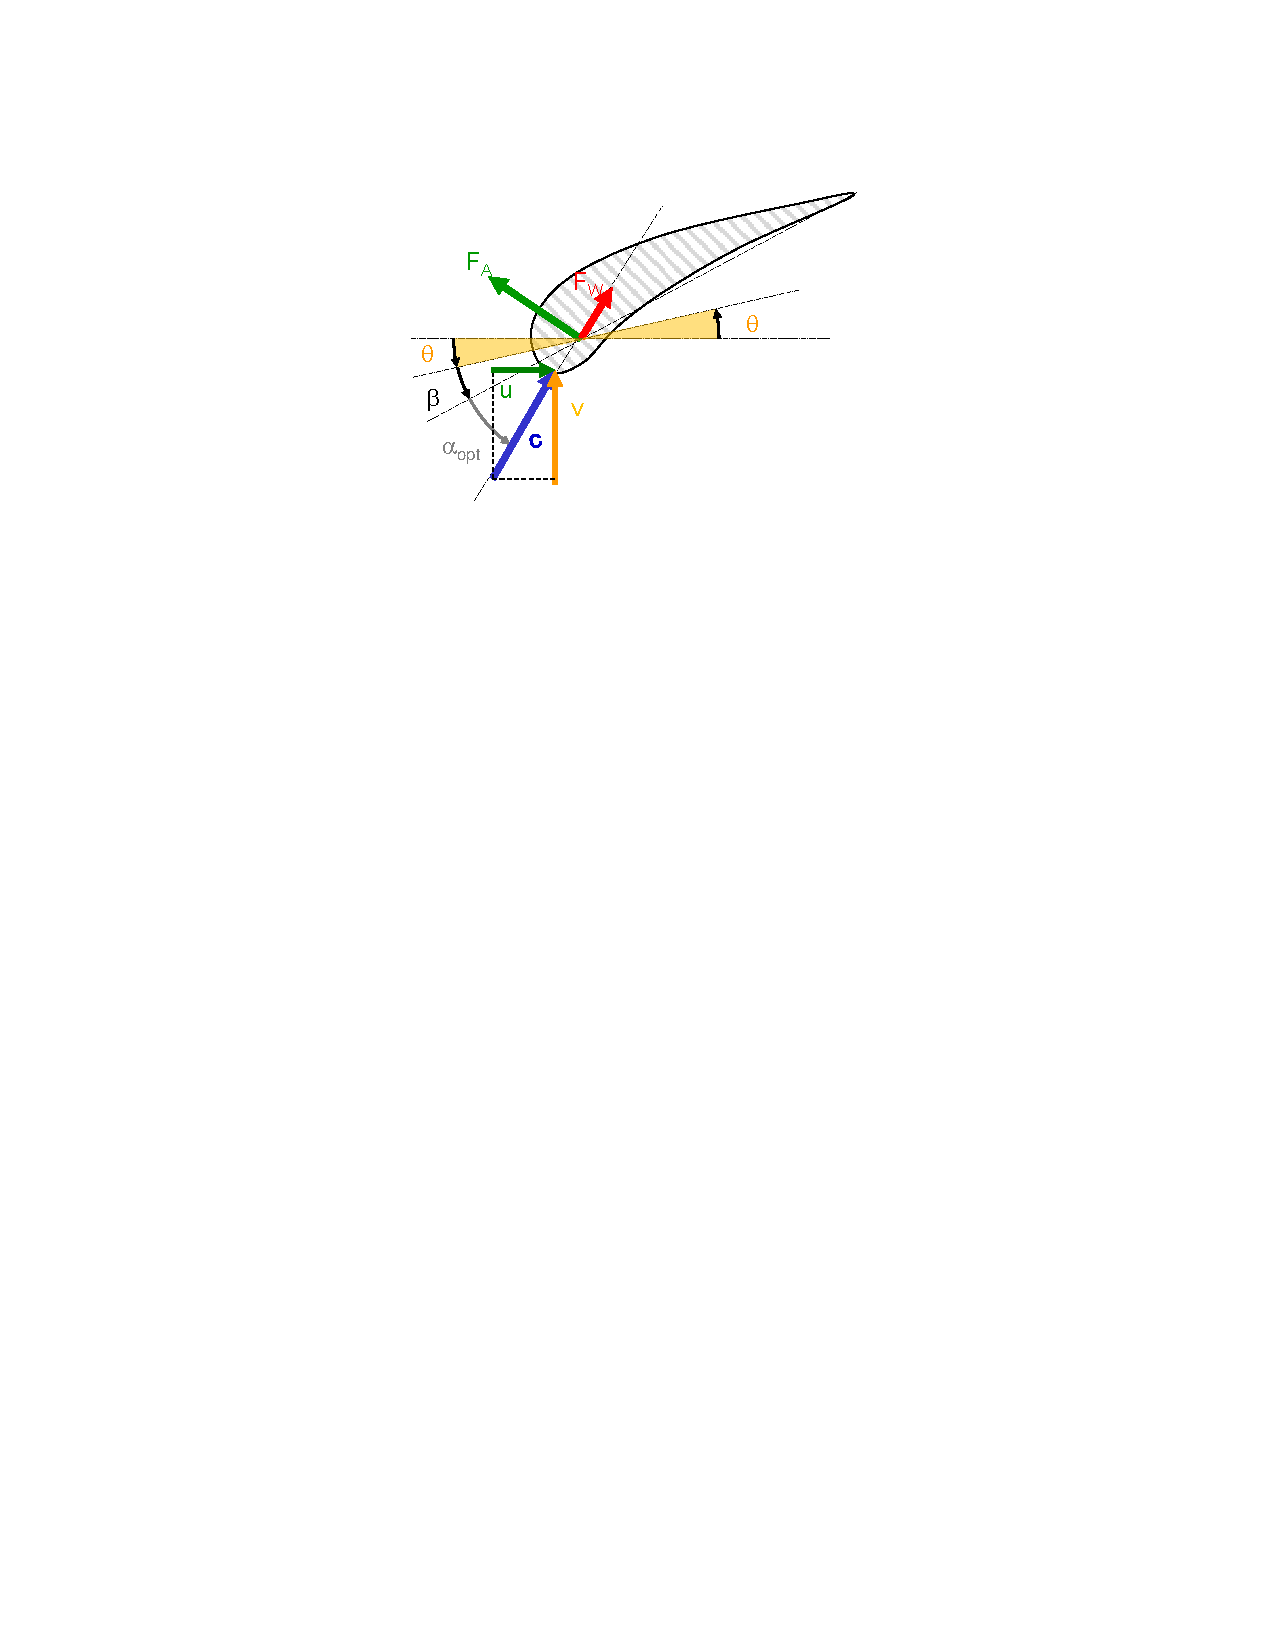
\includegraphics[width=0.5\textwidth]{Bilder/Kapitel 2/pitchen.pdf}}
   \caption[Pitchwinkel]{Pitchwinkel \cite{SkriptSchulte}}
   \label{fig:Bild2.11}
\end{figure}

Da die Drehung jedoch eine langsame Stellgröße darstellt und die Windgeschwindigkeiten schnellen Änderungen unterliegen, ist das Pitchen lediglich zur Leistungsbegrenzung sinnvoll. Ein weiterer Nachteil ist, dass der optimale Anstellwinkel \acs{alphaopt} lediglich für ein Blattelement eingestellt wird, nicht aber für die gesamte Blattlänge.

\newpage
\paragraph{Leistungsoptimierung durch Drehzahlanpassung}\mbox{}\smallskip\\
Als Alternative zum Pitchen wird die Rotordrehzahl \acs{nR} und somit die Umfangsgeschwindigkeit \acs{u} entsprechend der Windgeschwindigkeiten in der Rotorebene nachgeführt, um ein optimales Anströmverhältnis und ein daraus resutlierenden optimalen Anstellwinkel \acs{alphaopt} zu garantieren (\autoref{fig:Bild2.12}). Der optimale Anstellwinkel hängt direkt vom Anströmwinkel ab, d.h. der Anstellwinkel ändert die Größe indirekt zur Rotordrehzahl. Durch die dynamische Drehzahlanpassung kann im Gegensatz zur Pitchwinkelverstellung der optimale Anstellwinkel für alle Blattelemente eingestellt werden.

\begin{figure}[H]
   \centering
   \fbox{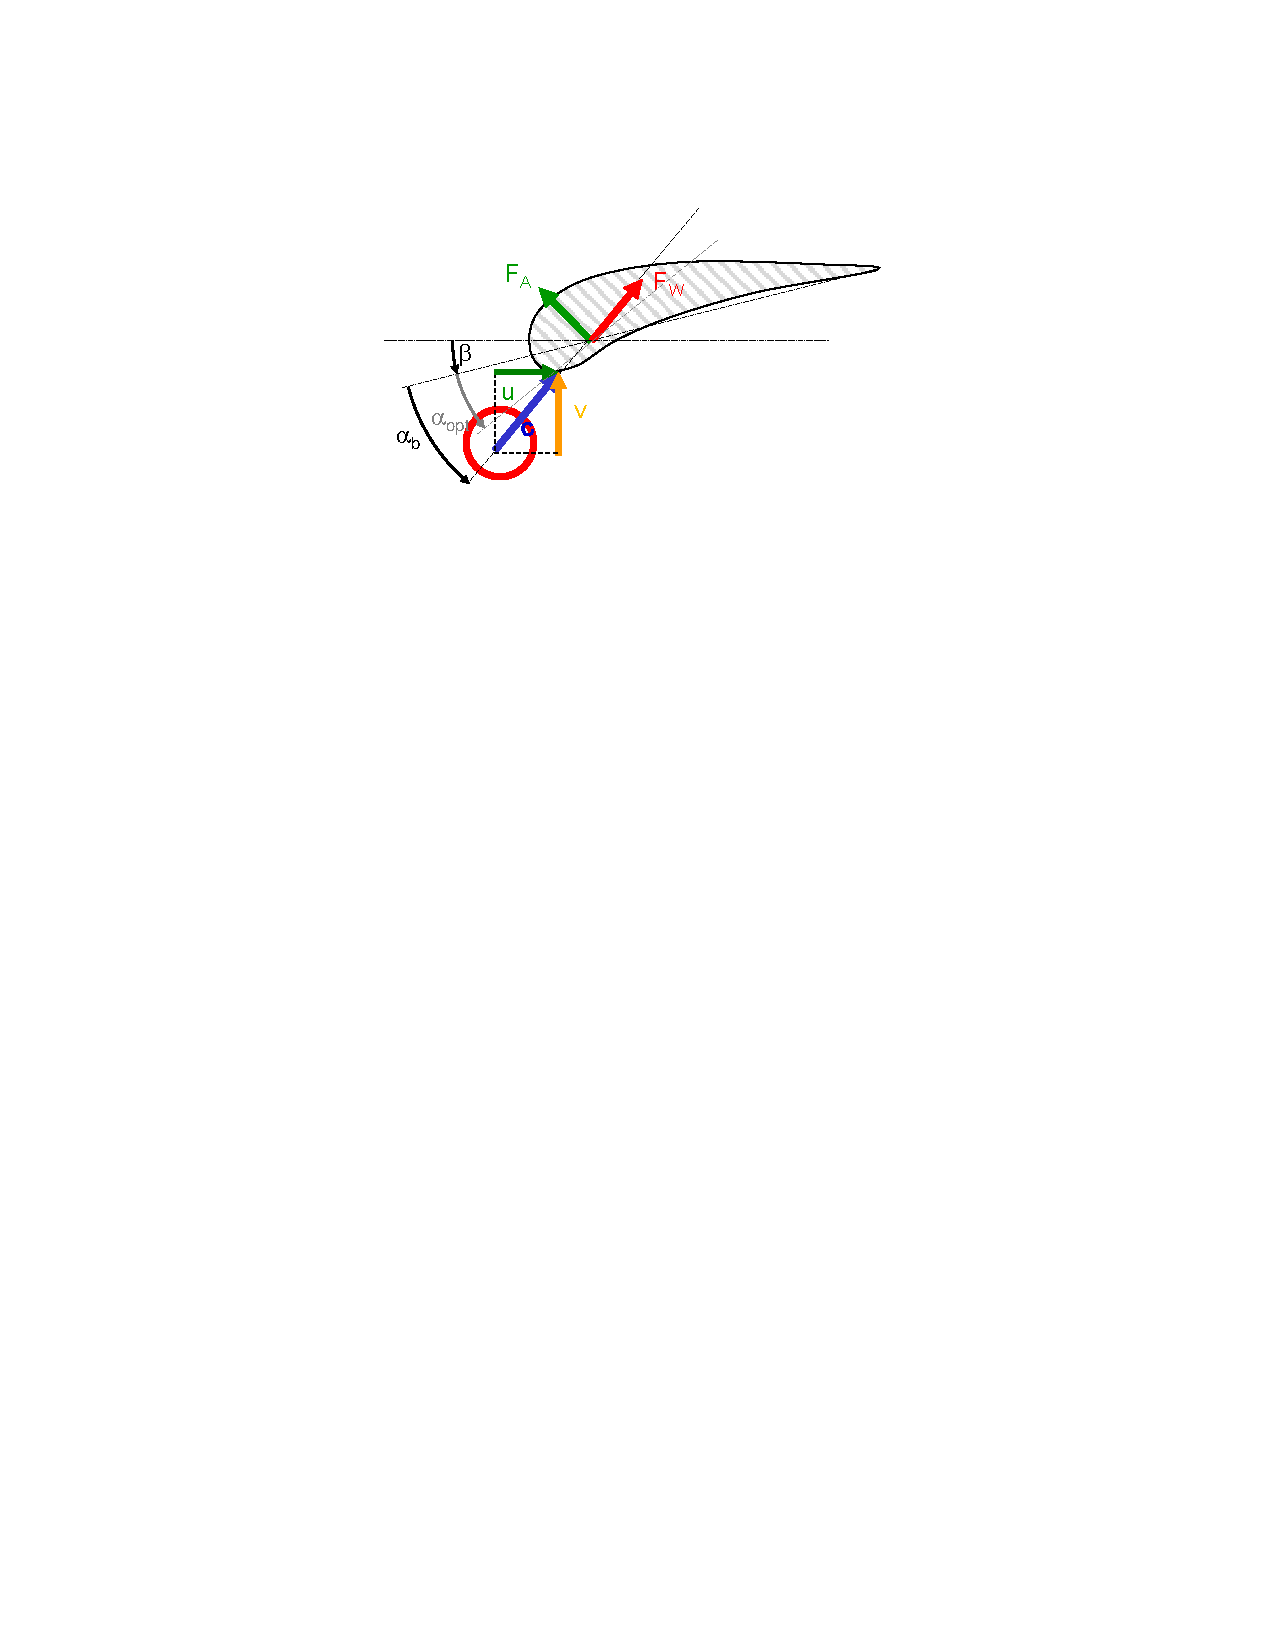
\includegraphics[width=0.5\textwidth]{Bilder/Kapitel 2/leistungsoptimierung_drehzahlanpassung.pdf}}
   \caption[Leistungsoptimierung durch Drehzahlanpassung]{Leistungsoptimierung durch Drehzahlanpassung \cite{SkriptSchulte}}
   \label{fig:Bild2.12}
\end{figure}

\subsection{Zusammenführung von Stromröhren- und Tragflügeltheorie}
Die Grundlage der Zusammenführung bildet der Leistungsbeiwert \acs{cP}, welcher das Verhältnis von Rotorleistung \acs{PR} zu Windleistung \acs{PW} widerspiegelt (\autoref{eq:Gleichung2.13}).\\
Die Rotorleistung folgt dabei aus den Kenntnissen der Tragflügeltheorie in Abhängigkeit der resultierend Umfangskraft $\acs{deltaFU}\left(\acs{alpha}, \acs{gamma}\right)$ (\autoref{eq:Gleichung2.28}). Die Berechnung der zur Verfügung stehenden Windenergie resultiert aus der Stromröhrentheorie (\autoref{eq:Gleichung2.6}). Durch die Zusammenführung ist ein Zusammenhang zwischen Anstellwinkel \acs{alpha} und dem Leistungsbeiwert \acs{cP} hergestellt worden.

\subsubsection{Zusammenhang zwischen Anstellwinkel und Leistungsbeiwert}
Der Anstellwinkel \acs{alpha} bestimmt die Größe der Gleitzahl \acs{eps} (\autoref{eq:Gleichung2.18}), welche das Verhältnis von Antriebskraft $\acs{FA}\left(\acs{alpha}\right)$ zu Widerstandskraft $\acs{FW}\left(\acs{alpha}\right)$ bzw. der beiden Beiwerte $\acs{cA}\left(\acs{alpha}\right)$ und $\acs{cW}\left(\acs{alpha}\right)$ widergibt. Bei einem optimalen Anstellwinkel \acs{alphaopt} wird dieses Verhältnis ebenfalls optimal und somit auch die Gleitzahl \acs{epsopt}.
\begin{equation*}
    \acs{alpha} \rightarrow \acs{alphaopt} \Rightarrow \acs{eps} \rightarrow \acs{epsopt}
\end{equation*}

Die resultierende Umfangskraft $\acs{deltaFU}\left(\acs{alpha}, \acs{gamma}\right)$ erreicht aufgrund der Abhängigkeit zu den Beiwerten ebenfalls das Optimum, wenn die Gleitzahl im Optimum ist.
\begin{equation*}
    \acs{epsopt} \Rightarrow \acs{deltaFU}_{\mathrm{opt}}
\end{equation*}
\newline
Da die notwendige Rotorleistung von der Umfangskraft abhängt, führt eine Steigerung der Umfangskraft \acs{deltaFU} zu einer einer Steigerung der Rotorleistung \acs{PR}.
\begin{equation*}
    \acs{deltaFU}\uparrow \Rightarrow \acs{PR}\uparrow
\end{equation*}
\newline
Durch den Anstieg der Rotorleistung, steigt das Verhältnis von Rotorleistung zu Windleistung und somit der Leistungsbeiwert \acs{cP}.
\begin{equation*}
    \acs{PR}\uparrow \Rightarrow \acs{cP}\uparrow
\end{equation*}
\newline
Somit wird geschlussfolgert, dass ein optimaler Anstellwinkel \acs{alphaopt} zu einem optimalen Leistungsbeiwert \acs{cPopt} führt. Da der Zusammenhang über die nicht monotone Funktion der Gleitzahl \acs{eps} hergestellt wurde, ist die Änderung des Leistungsbeiwertes \acs{cP} nicht proportional zu einer Änderung des Anstellwinkels \acs{alpha}.

\subsubsection{Momentenbeiwert \acs{cM}}
Der Momentenbeiwert \acs{cM} wird als Quotient aus Leistungsbeiwert \acs{cP} und Schnellaufzahl \acs{lambda} definiert (\autoref{eq:Gleichung2.33}).
\begin{equation}\label{eq:Gleichung2.33}
    \boxed{\acs{cM} = \frac{\acs{cP}}{\acs{lambda}}}
\end{equation}
\newline
Aus den Kenntnissen über die Zusammenhänge von Leistungen und Momenten (\autoref{eq:Gleichung2.34} und \autoref{eq:Gleichung2.35}) folgt bei Gleichsetzung der Rotor- und Windleistung, dass der Momentenbeiwert ebenfalls den Quotienten aus Rotormoment \acs{MR} zu Windmoment \acs{MW} repräsentiert (\autoref{eq:Gleichung2.36}).
\begin{align}
    \acs{PW} &= \acs{MW} \cdot \acs{omegaR} \cdot \acs{cM} \label{eq:Gleichung2.34} \\
    \acs{PR} &= \acs{MR} \cdot \acs{omegaR} \label{eq:Gleichung2.35}
\end{align}
\begin{equation}\label{eq:Gleichung2.36}
    \boxed{\acs{cM} = \frac{\acs{MR}}{\acs{MW}}}
\end{equation}

\subsubsection{Zusammenfassung der Leistungen und Drehmomente von Rotor und Wind}
Das Winddrehmoment resultiert aus dem Produkt von Schukraft \acs{FST} und Blattradius \acs{R}. Zur Berechnung der Windleistung  gilt \autoref{eq:Gleichung2.7}.
\begin{align*}
    \acs{MW} = \acs{FST} \cdot \acs{R}
\end{align*}
\begin{equation}\label{eq:Gleichung2.37}
    \boxed{\acs{MW} = \frac{1}{2} \cdot \acs{rho} \cdot \acs{v1}^2 \cdot \acs{A2} \cdot \acs{R}}
\end{equation}
\newline
\begin{align*}
    \acs{PW} = \acs{FST} \cdot \acs{v1}
\end{align*}
\begin{equation}\label{eq:Gleichung2.38}
    \boxed{\acs{PW} = \frac{1}{2} \cdot \acs{rho} \cdot \acs{v1}^3 \cdot \acs{A2}}
\end{equation}
\newline
Die Gleichungen zur Berechnung des Rotordrehmoments \acs{MR} und der Rotorleistung \acs{PR} ruhen auf Basis von \autoref{eq:Gleichung2.12} und \autoref{eq:Gleichung2.36}.
\begin{align*}
    \acs{MR} = \acs{FST} \cdot \acs{R} \cdot \acs{cM}
\end{align*}
\begin{equation}\label{eq:Gleichung2.39}
    \boxed{\acs{MR} = \frac{1}{2} \cdot \acs{rho} \cdot \acs{v1}^2 \cdot \acs{A2} \cdot \acs{R} \cdot \acs{cM}}
\end{equation}
\newline
\begin{align*}
    \acs{PR} = \acs{FST} \cdot \acs{v1} \cdot \acs{cP}
\end{align*}
\begin{equation}\label{eq:Gleichung2.40}
    \boxed{\acs{PR} = \frac{1}{2} \cdot \acs{rho} \cdot \acs{v1}^2 \cdot \acs{A2} \cdot \acs{v1} \cdot \acs{cP}}
\end{equation}

\subsection{WEA-Kennfelder} \label{kennfelder}
In den nachfolgenden Kapiteln werden die WEA-Kennfelder näher erläutert. Hierbei wird inbesondere auf die dimensionslosen Kennfelder eingegangen, da diese direkt verwendet werden. Die dimensionsbehafteten Kennfelder werden lediglich in der Theorie beschrieben und nicht mit grafischen Beispielen dargestellt.

\subsubsection{Kennlinien}
Zur Unterscheidung von leistungsoptimalen und leistungsbegrenzenden Arbeitsbereichen werden Rotorkennfelder aufgenommen. Diese visualisieren die aus dem Zusammenwirken von Rotor und Generator ergebenen Arbeitspunkte und beschreiben das Betriebsverhalten von Antriebs- und Arbeitsmaschinen. Der Verlauf von Kennfeldern kann von einem oder mehreren Parametern abhängen und somit als 2D oder nD-Plot aufgenommen werden. Sind in diesen die separaten Kennfelder von Arbeits- und Antriebsmaschine aneinander angepasst, kann beim Schnittpunkt beider ein stationärer Arbeitspunkt abgelesen werden, in dem ein Gleichgewicht des Systems vorliegt.\\
\newline
Im Fall der Leistungsoptimierung, d.h. bis zum Erreichen der optimalen Rotorleistung bei Nenngeschwindigkeit muss die veränderliche Generatorleistungskennlinie die Rotorleistungskennlinie so schneiden, dass der stationäre Arbeitspunkt stets im Optimum der Rotorleistungskennlinie liegt (\autoref{fig:Bild2.13}). Dies ist Teil der Reglerauslegung.
\begin{figure}[H]
   \centering
   \fbox{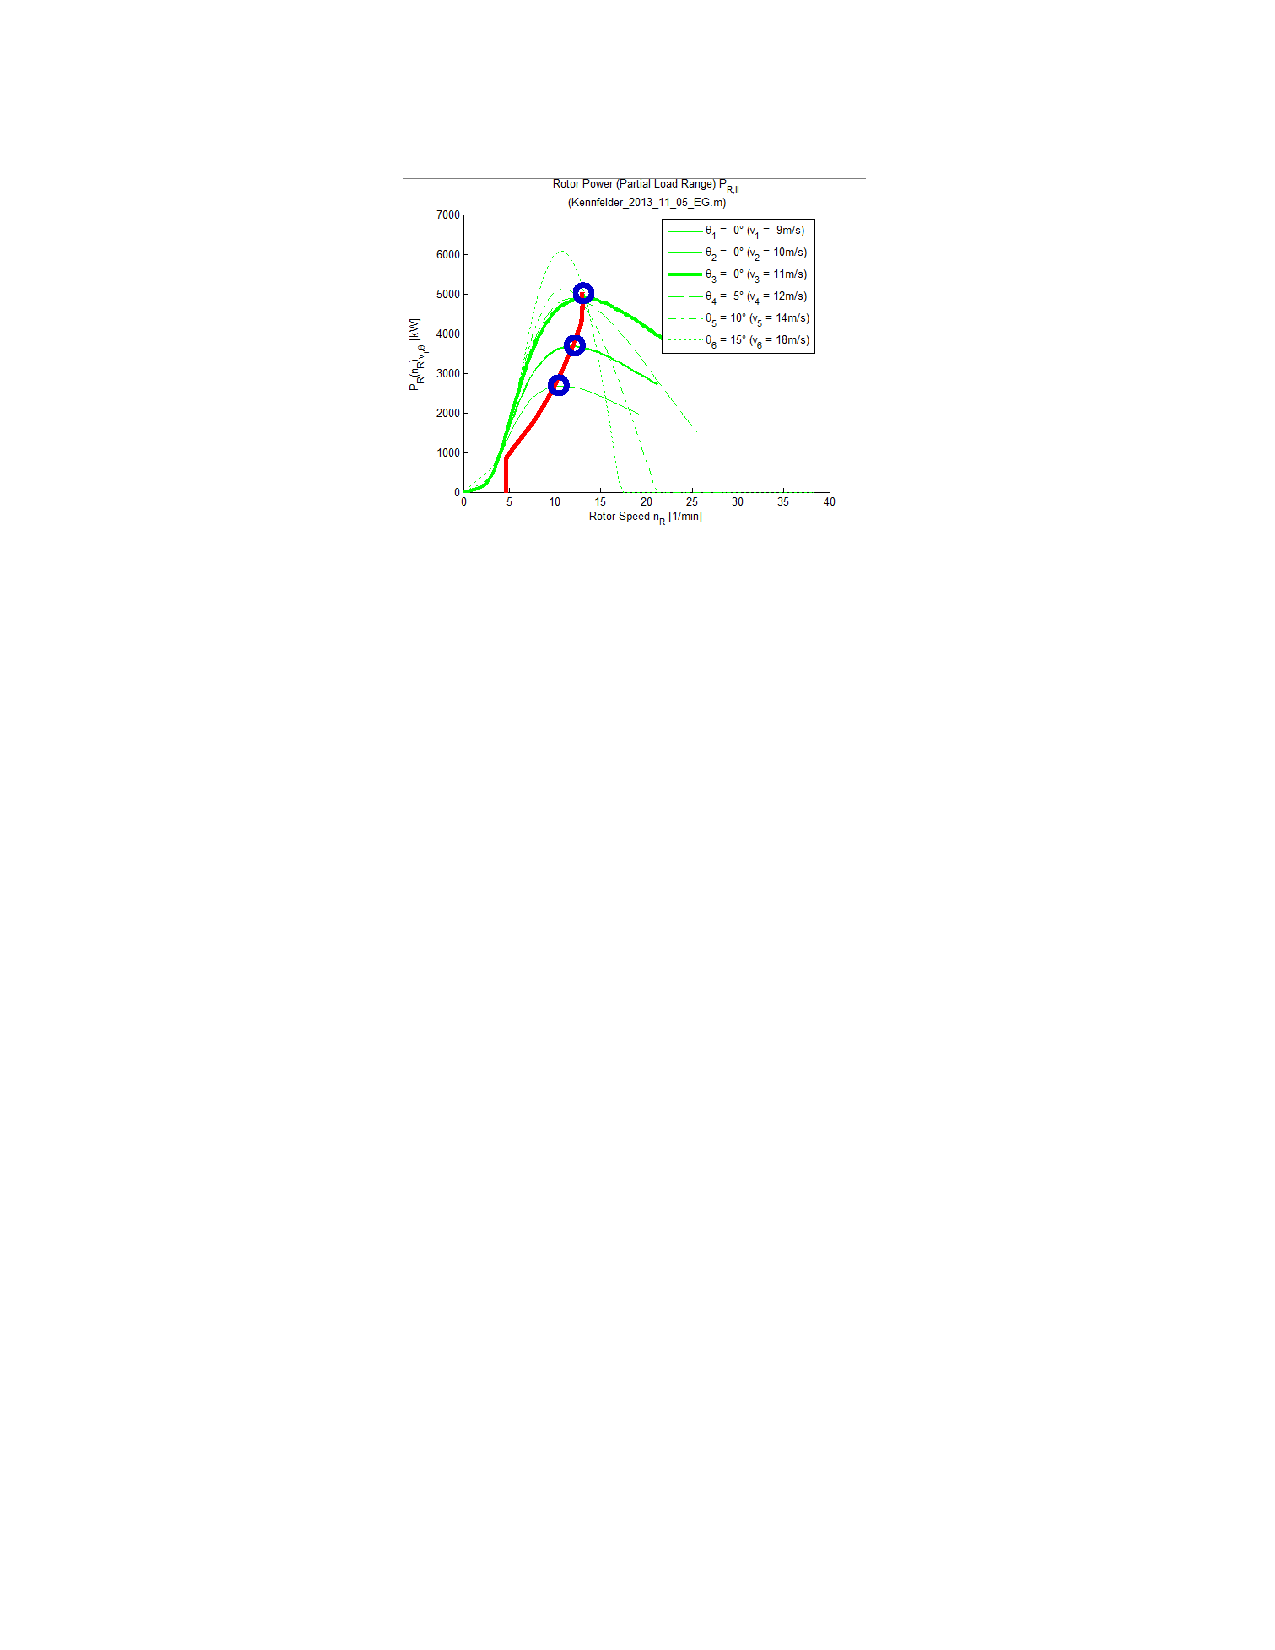
\includegraphics[width=0.7\textwidth]{Bilder/Kapitel 2/Leistungsoptimierung.pdf}}
   \caption[Arbeitspunkte bei Leistungsoptimierung]{Arbeitspunkte bei Leistungsoptimierung \cite{SkriptSchulte}}
   \label{fig:Bild2.13}
\end{figure}

Bei der Leistungsbegrenzung muss das Rotorkennfeld durch Pitchen verändert werden, dass alle Rotorkennlinien den Nennarbeitspunkt schneiden (\autoref{fig:Bild2.14}). Dies ist damit begründet, dass ein Generator nicht oberhalb der Nenndrehzahl \acs{nGNenn} bzw. des Nennmoments \acs{MGnenn} betrieben werden darf. Der Nennarbeitspunkt liegt vor, wenn die Generatordrehzahl \acs{nG}, die Generatorleistung \acs{PG}, als auch das Generatormoment \acs{MG} im Nennpunkt sind.
\begin{figure}[H]
   \centering
   \fbox{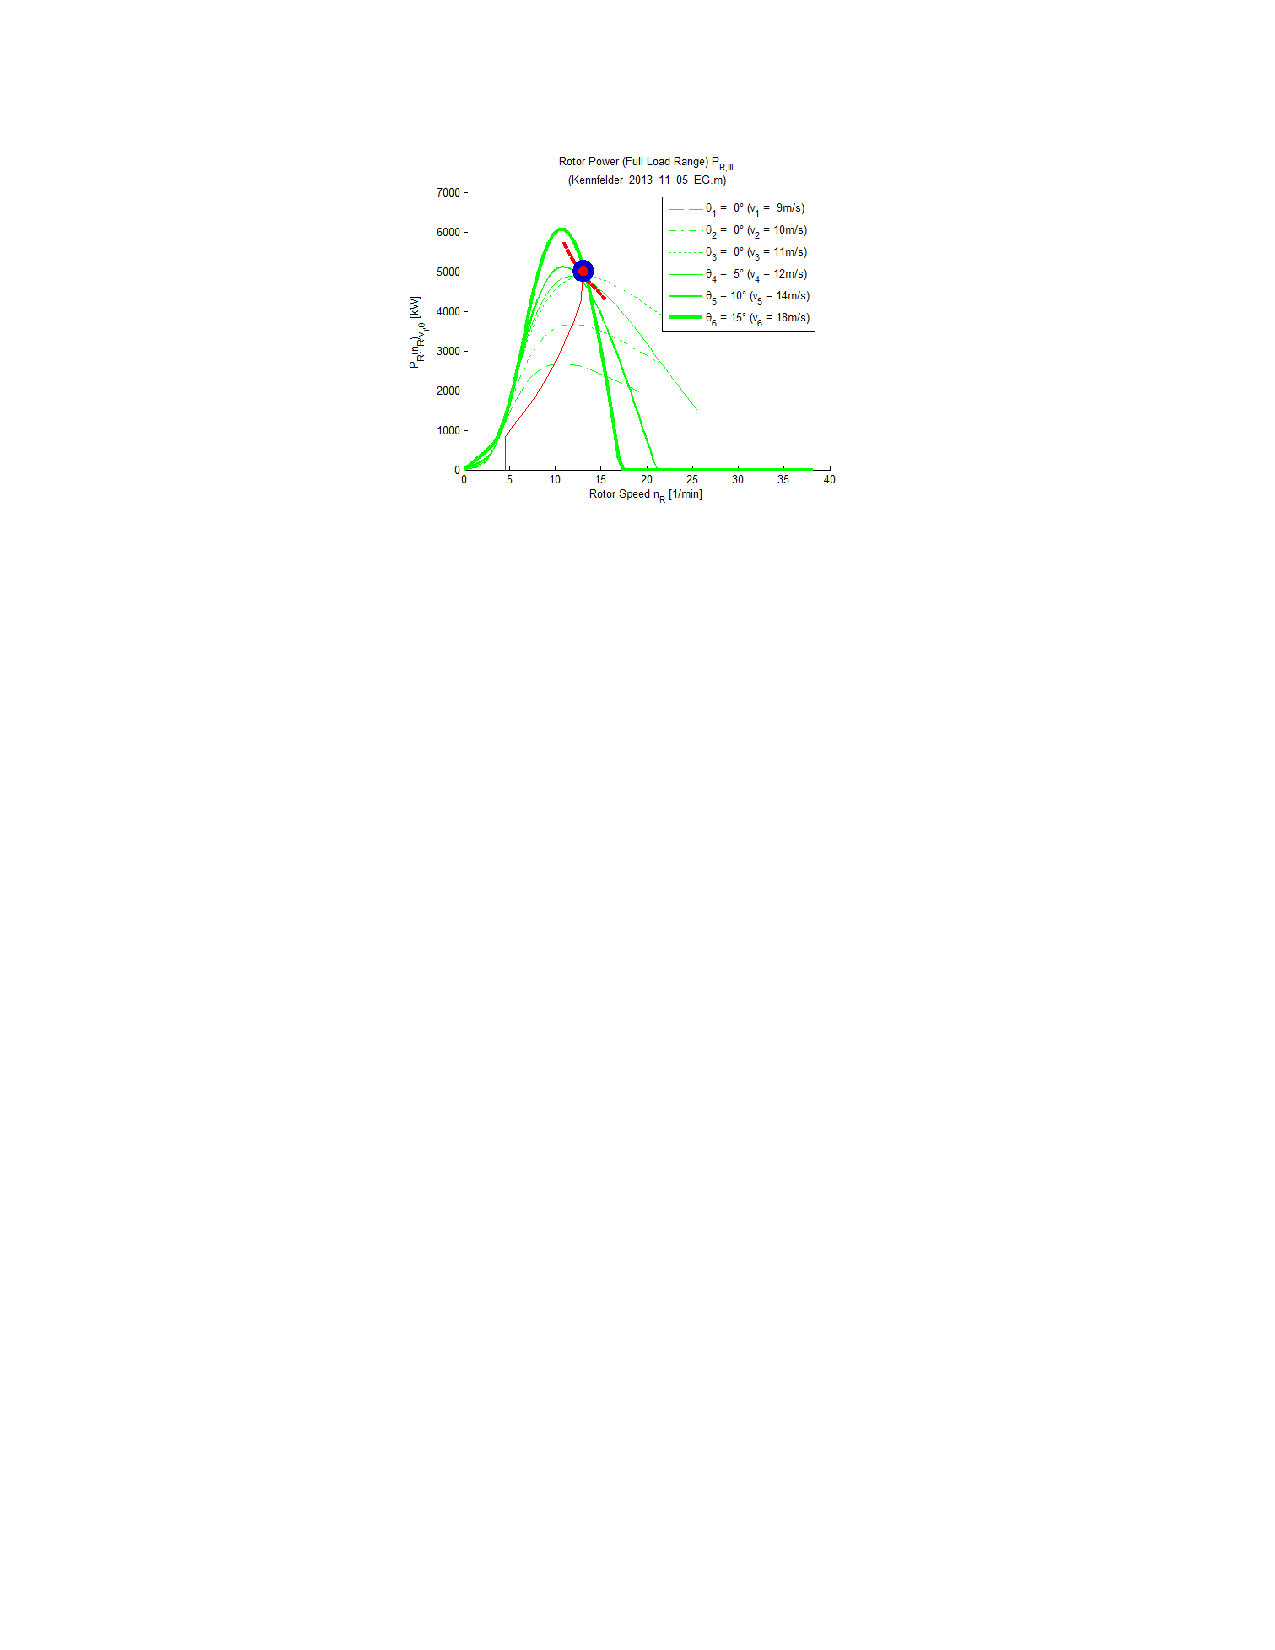
\includegraphics[width=0.7\textwidth]{Bilder/Kapitel 2/Leistungsbegrenzung.pdf}}
   \caption[Arbeitspunkte bei Leistungsbegrenzung]{Arbeitspunkte bei Leistungsbegrenzung \cite{SkriptSchulte}}
   \label{fig:Bild2.14}
\end{figure}

\subsubsection{Dimensionslose Rotorkennfelder}
Als dimensionslose Rotorkennfelder werden die Kennfelder der Leistungsbeiwerte \acs{cP} und der Momentenbeiwerte \acs{cM} bezeichnet, da diese von der dimensionslosen Schnelllaufzahl \acs{lambda} abhängen, welche wiederhum von der nicht beeinflussbaren Windgeschwindigkeit \acs{v1} bestimmt wird. Als weitere Parameter werden die Blattkontur und der Pitchwinkel \acs{theta} herangezogen. Alle drei Parameter beeinflussen den Anstellwinkel \acs{alpha}. Somit folgt eine Schar an Kurvenverläufen von Leistungsbeiwerten (\autoref{fig:Bild2.15}). Jede Blattkontur weist ein eigenes \acs{cP}-Kennfeld auf, welches dem WEA-Hersteller vom Blatt-Hersteller zur Reglerauslegung und Anlagenkonstruktion zur Verfügung gestellt wird.\\
\newline
Durch eine analytische Berechnung des Leistungsbeiwertes folgt:
\begin{align*}
    \acs{cP}\left(\acs{tflug}, \acs{bflug}, \acs{cA}, \acs{cW}, \acs{gamma}, \acs{lambdaopt}\right) = \acs{cP}\left(\acs{lambdaopt}\right)
\end{align*}

\begin{figure}[H]
   \centering
   \fbox{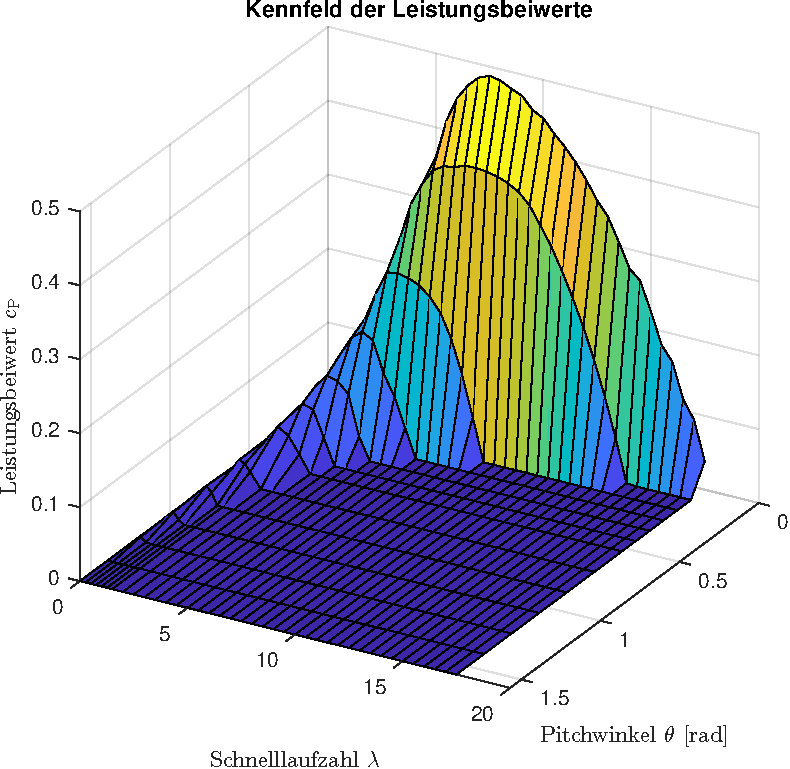
\includegraphics[width=0.7\textwidth]{Bilder/Kapitel 2/Kennfeld_Leistungsbeiwert.pdf}}
   \caption[Kennfeld der Leistungsbeiwerte]{Kennfeld der Leistungsbeiwerte}
   \label{fig:Bild2.15}
\end{figure}

Basierend auf der Umrechnung \autoref{eq:Gleichung2.33} kann das Kennfeld der Momentenbeiwerte \acs{cM} erstellt werden. Dieses sieht folgendermaßen aus (\autoref{fig:Bild2.16}).
\begin{figure}[H]
   \centering
   \fbox{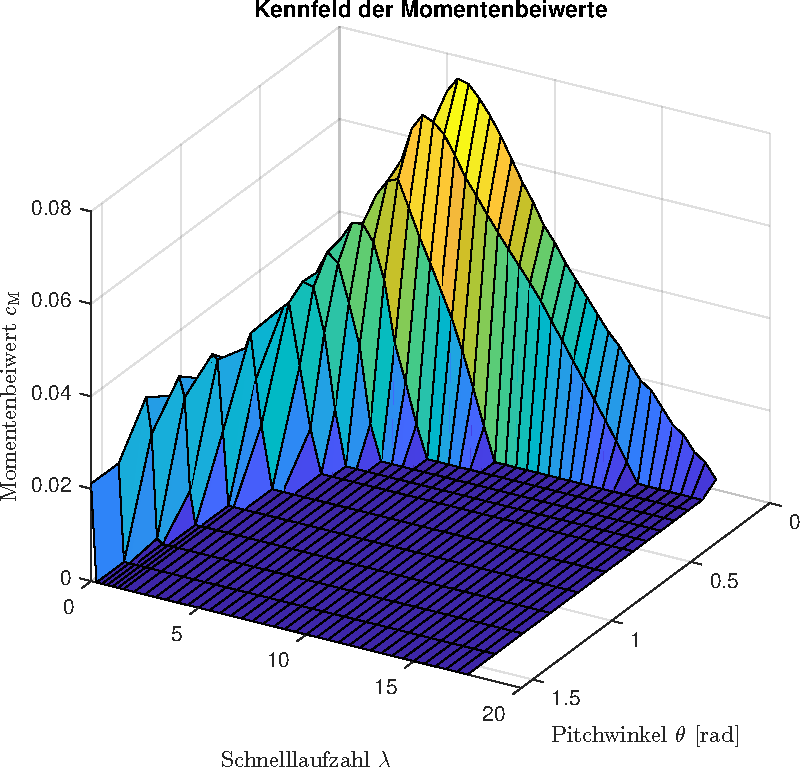
\includegraphics[width=0.7\textwidth]{Bilder/Kapitel 2/Kennfeld_Momentenbeiwert.pdf}}
   \caption[Kennfeld der Momentenbeiwerte]{Kennfeld der Momentenbeiwerte}
   \label{fig:Bild2.16}
\end{figure}

Im \acs{cM}-Kennfeld ist zu erkennen, dass im Rotorstillstand (\acs{lambda} = 0) ein Wert ungleich Null vorliegt. Durch die Beziehung aus \autoref{eq:Gleichung2.33} folgt ein \acs{cP}-Wert gleich Null. Weiter ist zu erkennen, dass das \acs{cP}-Kennfeld bis zum Optimum \acs{cPopt} ansteigt, welches bei \acs{lambdaopt} liegt. Selbiges ist im \acs{cM}-Kennfeld sichtbar. Die erreichte Schnelllaufzahl im Optimum ist hier jedoch kleiner als im \acs{cP}-Kennfeld. Für Schnellaufzahlen größer als das jeweilige Optimum, fallen beide Kennfelder wieder ab. Durch Vergrößerung des Pitchwinkels \acs{theta} folgt eine Reduktion des maximalen Leistungs- bzw. Momentenbeiwertes durch den Übergang in die Leistungsbegrenzung.\\
Der Pitchwinkel als auch die Schnelllaufzahl haben über das Kennfeld der Schubkraftbeiwerte \acs{cT} Einfluss auf die Schubkraft \acs{FS}, welche Auswirkung auf die Turm- und Blattauslenkung hat. Dies ist ebenso ein dimensionsloses Kennfeld und wird hier zur Vollständigkeit dargestellt (\autoref{fig:Bild2.17}).
\begin{figure}[H]
   \centering
   \fbox{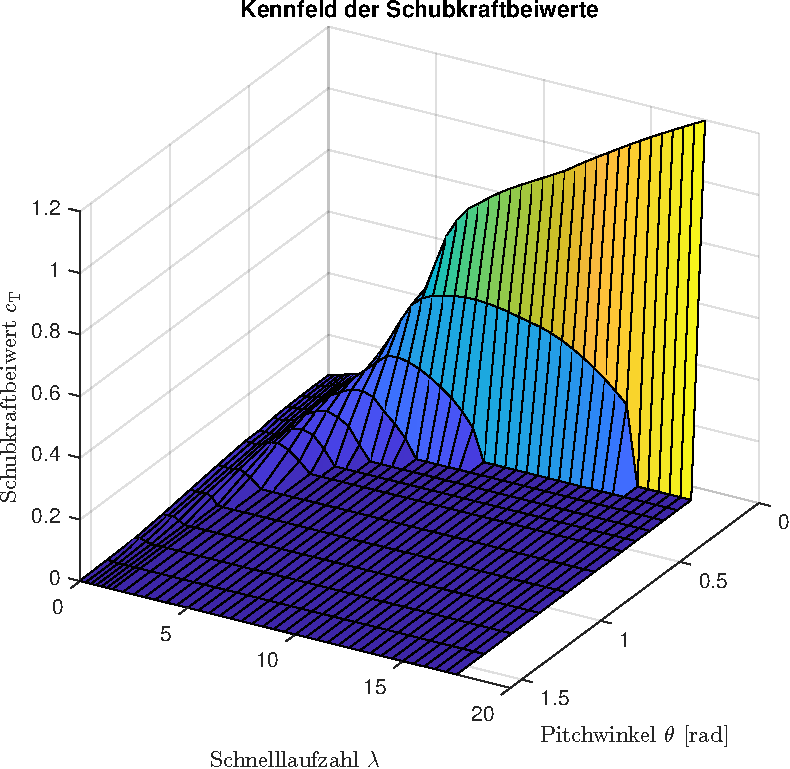
\includegraphics[width=0.7\textwidth]{Bilder/Kapitel 2/Kennfeld_Schubkraftbeiwert.pdf}}
   \caption[Kennfeld der Schubkraftbeiwerte]{Kennfeld der Schubkraftbeiwerte}
   \label{fig:Bild2.17}
\end{figure}

\subsubsection{Dimensionsbehaftete Rotorkennfelder}
Die in Kapitel 2.4.2 betrachteten dimensionslosen Rotorkennfelder können in dimensionsbehaftete Rotorkennfelder umgerechnet werden. Diese hängen von der Rotordrehzahl \acs{nR} ab, welche in Abhängigkeit der Schnelllaufzahl \acs{lambda} steht.
\begin{align*}
    \acs{nR} = \frac{\acs{v1}}{2\cdot\pi\cdot \acs{R}}\cdot\lambda
\end{align*}
\newline
Die Windgeschwindigkeit wird nun als Parameter vorgegeben, wonach nun die Rotordrehzahl \acs{nR} als Variable gilt. Die Berechnung der Rotorleistung und des Rotordrehmoments erfolgt mithilfe der \autoref{eq:Gleichung2.39} und \autoref{eq:Gleichung2.40}. Auf Grundlage der Rotorleistung in Abhängigkeit der Rotordrehzahl kann über das Getriebeübersetzungsverhältnis die Generatorleistung bestimmt werden.


\section{Modell des Antriebsstranges} \label{modellierung_antriebsstrang}
% Aaron

Dieser Abschnitt befasst sich mit der Modellierung und Simulation des Antriebsstranges der Windturbine. Das Modell soll anschließend zusammen mit dem Modell des Turmes und des Blattes, sowie der Aerodynamik als Teilmodelle in Simulink zusammengeführt werden. \\
Der Antriebsstrang besteht dabei grundsätzlich aus einem Rotor (Blätter und Nabe), einem Getriebe, einem Synchrongenerator sowie einer Welle, welche alle Komponenten mechanisch verbindet. \autoref{fig:Bild3.1} zeigt einer Übersichtsgrafik der Modellparameter als Ein- \bzw Ausgänge des Teilmodells.

\begin{figure}[H]
   \centering
   \begin{pspicture}[showgrid=false](0,0)(10,5)
        \psframe(0,0)(10,5)
        % Eingänge
        \psline{->}(1,3.5)(3.5,3.5)
        \rput(1,3.9){\footnotesize \acs{MG}}
        \psline{->}(1,2.5)(3.5,2.5)
        \rput(1,2.9){\footnotesize \acs{MR}}
        % Modell
        \psframe[linecolor=black,fillcolor=lightGrey,fillstyle=solid](3.5,0.5)(6.5,4.5)
        \rput(5,3.5){\small Modell des}
        \rput(5,3){\small Antriebsstranges}
        % Ausgänge
        \psline{->}(6.5,3.5)(9,3.5)
        \rput(9,3.9){\footnotesize \acs{omegaG}}
        \psline{->}(6.5,2.5)(9,2.5)
        \rput(9,2.9){\footnotesize \acs{omegaR}}
    \end{pspicture}
   \caption[Übersicht Antriebsstrangteilmodell]{Blockdarstellung des Antriebsstrangteilmodells inklusive der Ein- und Ausgangsparameter}
   \label{fig:Bild3.1}
\end{figure} % Teilmodell Antriebsstrang mit Ein- und Ausgangsparametern

Zu erkennen sind das \ac{MG} und das \ac{MR} als Eingangsgrößen des Modells. Das \acl{MR} wird in der Gesamtsimulation später vom Modell der Aerodynamik bereitgestellt. Das \acl{MG} geht aus dem Generator-Umrichter-Modell hervor, in welchem auch die Regelung der Windkraftanlage umgesetzt ist. \\
Als Ausgänge benötigt werden die \ac{omegaG} und die \ac{omegaR}. Erstere ist später ein Eingangsparameter des Generator-Umrichter-Modells und wird insbesondere für die Berechnung des \acl{MG} im Momentenregler benötigt. Die \acl{omegaR} ist ebenfalls ein Eingang des Generator-Umrichter-Modells sowie des Modells für die Aerodynamik. 

\subsection{Modellierung des Antriebsstranges}

Zunächst soll das Modell für den Antriebsstrang entwickelt werden, bevor es anschließend simulativ losgelöst in Simulink getestet und verifiziert werden kann. \autoref{fig:Bild3.2} zeigt modellhaft die Struktur des Antriebsstranges mitsamt der wirkenden Momente. Auf Basis der Abbildung erfolgt anschließend die Modellierung des Teilsystems.

\begin{figure}[H]
   \centering
   \begin{pspicture}[showgrid=false](0,0)(14.6,5)
        \psframe(0,0)(14.6,5)
        
        % Generator
        \psline(0.5,2.5)(2.1,2.5)
        \psarc[linecolor=darkgrey]{<-}(2,2.5){1}{150}{210}
        \rput(1.2,3.3){\footnotesize \acs{MG}}
        
        \psellipse(2.1,2.5)(0.3,0.61)
        \psline(2.1,3.1)(3.6,3.1)
        \psline(2.1,1.9)(3.6,1.9)
        \psarc(3.08,2.5){0.8}{-49}{49}
        \rput(3,2.5){\footnotesize \acs{JG}}
        
        \psline(3.9,2.5)(5,2.5)
        \psarc[linecolor=darkgrey]{<-}(3.6,2.5){1}{-30}{30}
        \rput(4.4,3.3){\footnotesize \acs{phiG}}
        
        % Dämpferglied
        \psline(5,3.1)(5,1.9)
        \pscoil[coilwidth=0.3](5,3.1)(7.05,3.1)
        \psline(5,1.9)(5.8,1.9)
        \psline(5.8,2.2)(5.8,1.6)
        \psline(5.8,2.2)(6.5,2.2)
        \psline(5.8,1.6)(6.5,1.6)
        \psline(6,2.15)(6,1.65)
        \psline(6,1.9)(7.05,1.9)
        \psline(7.05,3.1)(7.05,1.9)
        \rput(6,3.7){\footnotesize \acs{ks}}
        \rput(6,1.2){\footnotesize \acs{ds}}
        
        % Getriebe
        \psline(7.05,2.53)(8.1,2.53)
        \psline(7.05,2.47)(8.1,2.47)
        \psarc[linecolor=darkgrey]{<-}(6.7,2.5){1}{-30}{30}
        \rput(7.5,3.3){\footnotesize \acs{phiRtilde}}
        
        \psframe(8.1,1.9)(9.8,3.1)
        \rput(8.9,2.5){\footnotesize \acs{ng}}
        
        % Rotor
        \psline(9.8,2.53)(11.1,2.53)
        \psline(9.8,2.47)(11.1,2.47)
        \psarc[linecolor=darkgrey]{<-}(9.4,2.5){1}{-30}{30}
        \rput(10.2,3.3){\footnotesize \acs{phiR}}
        
        \psellipse(11.1,2.5)(0.3,0.61)
        \psline(11.1,3.1)(12.6,3.1)
        \psline(11.1,1.9)(12.6,1.9)
        \psarc(12.08,2.5){0.8}{-49}{49}
        \rput(11.98,2.5){\footnotesize \acs{JR}}
        
        \psline(12.9,2.5)(14,2.5)
        \psarc[linecolor=darkgrey]{<-}(12.4,2.5){1}{-30}{30}
        \rput(13.2,3.3){\footnotesize \acs{MR}}
    \end{pspicture}
   \caption[Modelldarstellung des Antriebsstranges]{Modellhafte des Antriebsstrangteilmodelles inklusive der wirkenden Momente}
   \label{fig:Bild3.2}
\end{figure} % Modelldarstellung des Antriebsstranges inkl. Momente

Die Modellbildung erfolgt über die Momentenbilanzierung. Diese besagt, dass die Summe aller wirkenden Momente gleich Null ist. Zunächst lässt sich die Summe aller Momente allgemein berechnen zu

\begin{align}
    \sum M = J \cdot \ddot\varphi.
    \label{eq:Gleichung3.1}
\end{align}

Nachfolgend wird eine Bilanzgleichung für den Generator (high speed shaft) und den Rotor (slow speed shaft) aufgestellt. Erstere ist in \autoref{eq:Gleichung3.2} und Letzere in \autoref{eq:Gleichung3.3} dargestellt.

\begin{align}
    \label{eq:Gleichung3.2}
   \acs{JR} \cdot \ddot{\varphi}_{\mathrm{R}} + \tilde{M}_{d_s} + \tilde{M}_{k_s} - \acs{MR} &= 0 \\
   \label{eq:Gleichung3.3}
   \acs{JG} \cdot \ddot{\varphi}_{\mathrm{G}} - {M}_{d_s} - {M}_{k_s} + \acs{MG} &= 0
\end{align}

Bei $\tilde{M}_{d_s}$ handelt es sich um das Moment, welches sich aus dem \ac{ds} ergibt. Es wird berechnet zu

\begin{align}
   \tilde{M}_{d_s} = \acs{ds} \cdot \left( \dot\varphi_{\mathrm{G}} - \tilde{\dot\varphi}_{\mathrm{R}}\right).
   \label{eq:Gleichung3.4}
\end{align}

Bei $\tilde{M}_{k_s}$ wiederum handelt es sich um das Moment, welches sich aus dem \ac{ks} ergibt. Dieses wird berechnet zu

\begin{align}
   \tilde{M}_{k_s} = \acs{ks} \cdot \left( \varphi_{\mathrm{G}} - \tilde{\varphi}_{\mathrm{R}}\right).
   \label{eq:Gleichung3.5}
\end{align}

Da es sich bei beiden Momenten um bezogene Größen (bezogen auf die Schnelle Welle) handelt, müssen diese noch umgerechnet werden. Dies geschieht über die \ac{ng}. $M_{d_s}$ und $M_{k_s}$ folgen somit zu

\begin{align}
    \label{eq:Gleichung3.6}
   M_{d_s} &= \acs{ng} \cdot \tilde{M}_{d_s} \\
   \label{eq:Gleichung3.7}
   M_{k_s} &= \acs{ng} \cdot \tilde{M}_{k_s}.
\end{align}

Auch bei $\tilde{\dot\varphi}_{\mathrm{R}}$ muss das Getriebeübersetzungsverhältnis wie folgt berücksichtigt werden:

\begin{align}
    \tilde{\dot\varphi}_{\mathrm{R}} = \acs{ng} \cdot \acs{phiR}
    \label{eq:Gleichung3.8}
\end{align}

Somit kann der Antriebsstrang abschließend modelliert werden zu

\begin{equation}
    \label{eq:Gleichung3.9}
   \boxed{\acs{JR} \cdot \ddot{\varphi}_{\mathrm{R}} + \acs{ng} \cdot \acs{ds} \cdot \left( \dot\varphi_{\mathrm{G}} - \acs{ng} \cdot \tilde{\dot\varphi}_{\mathrm{R}}\right) + \acs{ng} \cdot \acs{ks} \cdot \left( \varphi_{\mathrm{G}} - \acs{ng} \cdot \tilde{\varphi}_{\mathrm{R}}\right) - \acs{MR} = 0}
\end{equation}

\begin{equation}
   \label{eq:Gleichung3.10}
   \boxed{\acs{JG} \cdot \ddot{\varphi}_{\mathrm{G}} - \acs{ds} \cdot \left( \dot\varphi_{\mathrm{G}} - \acs{ng} \cdot \tilde{\dot\varphi}_{\mathrm{R}}\right) - \acs{ks} \cdot \left( \varphi_{\mathrm{G}} - \acs{ng} \cdot \tilde{\varphi}_{\mathrm{G}}\right) - \acs{MG} = 0}.
\end{equation}
\clearpage

\subsection{Simulative Modellverifikation des Antriebsstranges}

In diesem Unterkapitel wird das zuvor entwickelte Modell in Simulink implementiert und getestet. Auf eine Vollständige Verifikation wird an dieser Stelle jedoch verzichtet, da diese erst nach der Integration in das Gesamtsystem (mit allen anderen Teilmodellen) erfolgen kann. Geprüft wird jedoch, wie sich die Winkelgeschwindigkeiten des Rotors und des Generators nach einer sprunghaften Anregung verhalten. Ebenfalls verifiziert wird, inwiefern eine Torsion der Antriebswelle auftritt, wenn sich das \acl{MG} und das \acl{MR} sprunghaft zeitversetzt ändern. \\

\begin{figure}[H]
   \centering
   \fbox{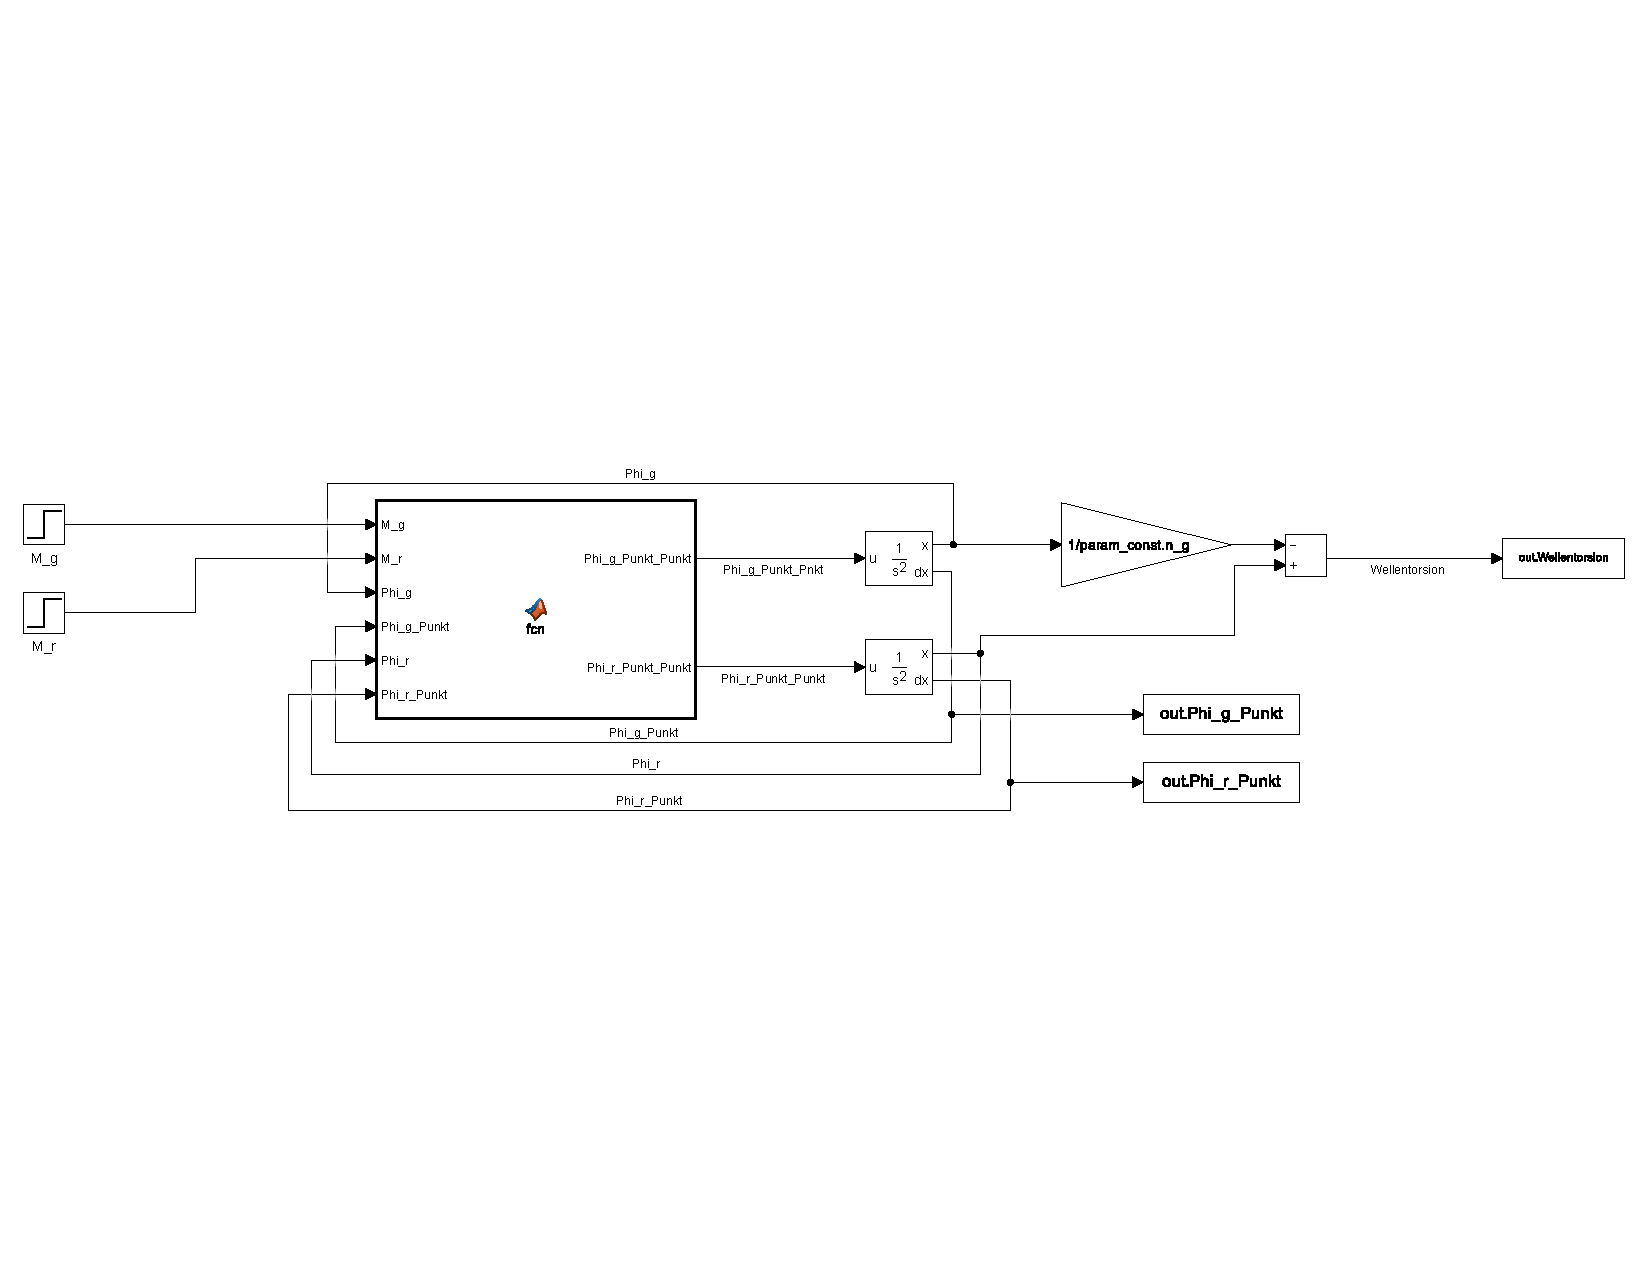
\includegraphics[width=1.0\textwidth]{Bilder/Kapitel 4/Blockstruktur_Antriebsstrang.pdf}}
   \caption[Antriebsstrang Simulink]{Simulink Blockstruktur des Antriebsstranges der WEA}
   \label{fig:Bild3.3}
\end{figure}

\autoref{fig:Bild3.3} zeigt die Blockstruktur, welche in Simulink umgesetzt wurde. Der Funktionsblock in der Mitte der Abbildung enthält die Modellgleichungen, welche zuvor in \autoref{eq:Gleichung3.1} und \autoref{eq:Gleichung3.1} hergeleitet wurden. Eingangsseitig wird ein Sprung von \acs{MG} \bzw \acs{MR} eingeprägt. Ersterer setzt nach \SI{15}{s} ein, Zweiterer bereits nach \SI{5}{s}. Ausgangsseitig werden durch die Nutzung von Integratoren die Winkelgeschwindigkeiten \acs{omegaR} und \acs{omegaG} zurückgegeben. Für die Modellverifikation wurde noch ein weiterer Ausgang hinzugefügt, welcher die Differenz des \ac{phiR} und des \ac{phiG} bereitstellt. \\

In \autoref{fig:Bild3.4} ist klar zu erkennen, dass durch die Einprägung des Momentensprunges auf den Rotor die Winkelgeschwindigkeit der Welle annähernd linear ansteigt. Dies zeigt sich sowohl auf Seiten des Rotors als auch auf Seiten des Generators. Der Kurvenverlauf beider Winkelgeschwindigkeiten ist annähernd identisch. Der Unterschied um zwei Zehnerpotenzen ergibt sich aus der \acf{ng}, welche bei \ca 100 (97) liegt.\\
Der generatorseitige Momentensprung zeigt sich in \autoref{fig:Bild3.4} besonders gut in der Betrachtung der \ac{dotphiG}. Es kommt zu einem Schwingvorgang, der nach etwas über \SI{5}{s} wieder ausgeglichen ist. Durch die Elastizität der Welle ist der Momentensprung am Generator rotorseitig abgedämpft. Die \ac{dotphiR} schwing nur leicht.

\begin{figure}[H]
   \centering
   \fbox{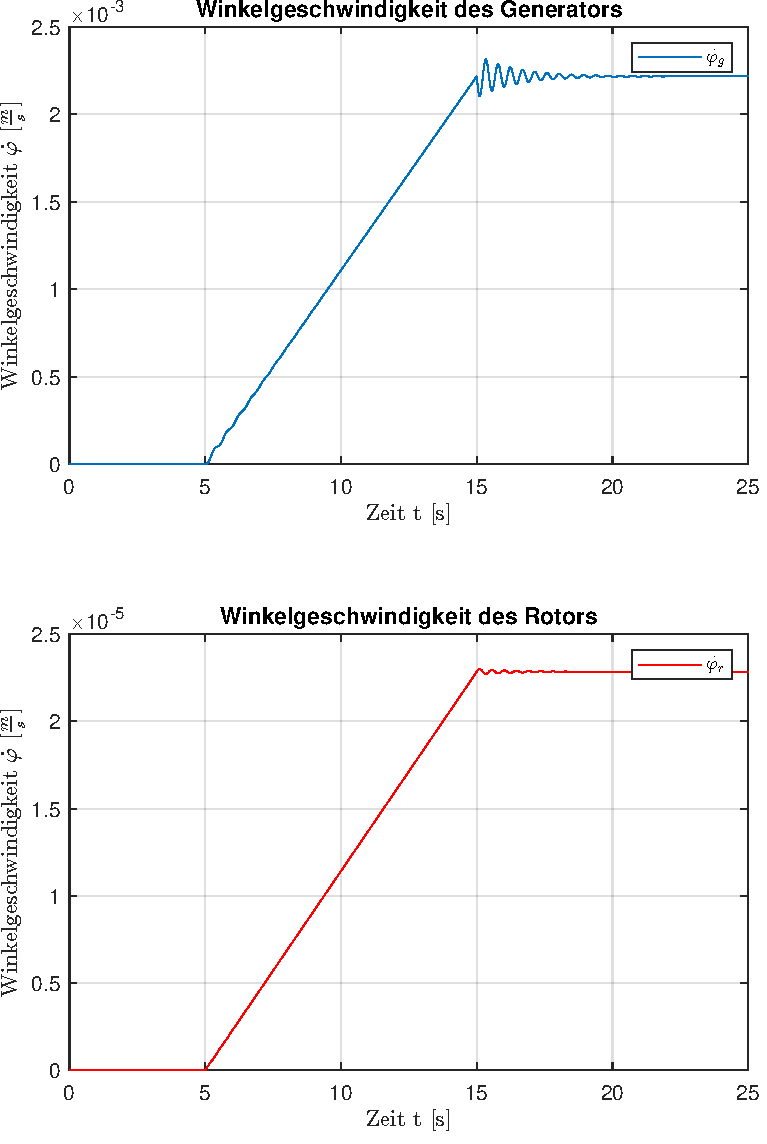
\includegraphics[width=0.76\textwidth]{Bilder/Kapitel 4/Winkelgeschwindigkeiten.pdf}}
   \caption[Winkelgeschwindigkeiten Antriebsstrang]{Visualisierung der Winkelgeschwindigkeit des Rotors und des Generators nach zeitversetzter Sprunganregung}
   \label{fig:Bild3.4}
\end{figure}

\autoref{fig:Bild3.5} zeigt die Differenz zwischen Rotorwinkel (\acs{phiR}) und Generatorwinkel (\ac{phiG}). Diese gibt eine Aussage darüber, inwiefern es zu einer Torsion der Antriebswelle kommt. Zu erkennen ist, dass nach \SI{5}{s} eine erste Torsion auftritt, die sich nach kurzem Schwingen auf einen stationären Wert von rund einem Millionstel eines Grades einpegelt. Nach dem generatorseitigen Momentensprung (bei \SI{15}{s} kommt es erneut zu einem Schwingvorgang in der Wellentorsion. Da das eingeprägte Moment signifikant größer ist, ist die Schwingungsamplitude ebenfalls deutlich größer als zuvor beim rotorseitigen Momentensprung. Nach \ca \SI{10}{s} ist auch dieser Schwingvorgang abgeschlossen und ein stationärer Endwert von rund einem Einhunderttausendstel Grad wird erreicht. \\
Es kann zusammenfassend argumentiert werden, dass die Simulationsergebnisse plausibel und hinreichend genau sind, um das Antriebsstrangmodell als Teilmodell der Simulation und Regelung der Windenergieanlage einsetzen zu können.

\begin{figure}[H]
   \centering
   \fbox{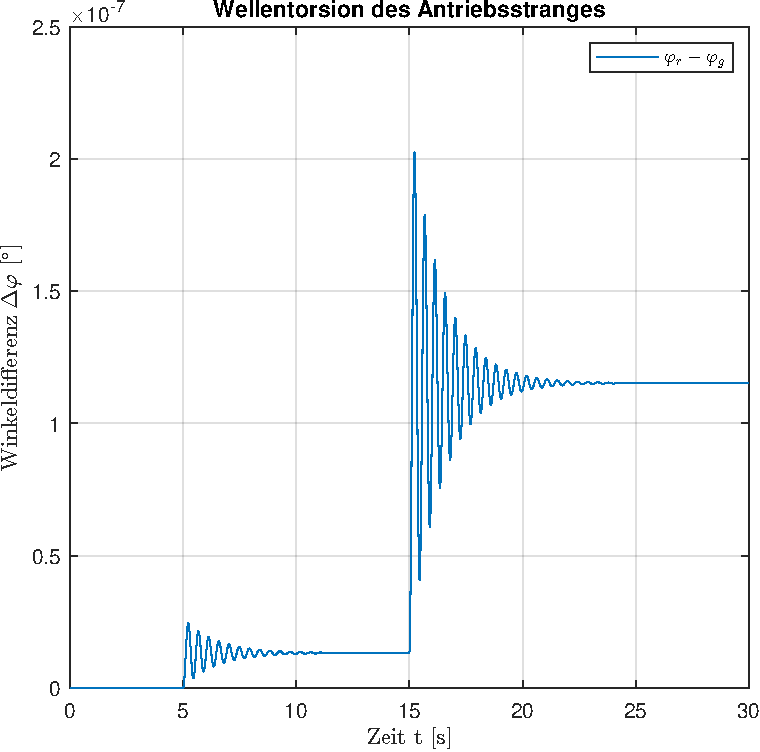
\includegraphics[width=0.76\textwidth]{Bilder/Kapitel 4/Wellentorsion.pdf}}
   \caption[Wellentorsion Antriebsstrang]{Visualisierung der Wellentorsion des Antriebsstranges nach zeitversetzter Sprunganregung}
   \label{fig:Bild3.5}
\end{figure}

\section{Momentenregelung des Antriebstranges} \label{regelung}
%Chris
\subsection{Regelungsziele und Regelkreis} \label{regelziel}
Bevor eine Regelung für die WEA umgesetzt werden kann, müssen zunächst einige Regelungsziele festgelegt werden. Aus der Beschreibung der Regelungsziele ergeben sich die Regelanforderungen der WEA. Des Weiteren wird die Komplexität des Reglers durch ein geeignetes Funktionsmodell, welches das dynamische Verhalten der Regelstrecke bestimmt, beschrieben. Hierfür wird das torsionsstarre Triebstrangmodell verwendet. Die Regelung konzentiert sich auf die Einhaltung und Umsetzung der Hauptziele, wobei das Verhalten der Blätter, des Turms und des Antriebsstranges nicht berücksichtigt werden. Folglich reicht ein sehr vereinfachtes Funktionsmodell aus. Aus der Generatorcharakteristik lassen sich insgesamt drei Arbeitsbereiche ermitteln, nämlich der untere und obere Teillastbereich, sowie der Volllastbereich. Die folgende \autoref{tab:Tabelle4.1} fasst die Hauptziele des Reglers zusammen. Auf Grundlage dessen, werden in den folgenden Kapiteln die benötigten Regler für die verschiedenen Arbeitsbereiche entwickelt.
\\


\begin{table}[H]
    \centering
    \begin{tabular}{|l|}
        \hline                                                        
        \rowcolor{lightGrey}
        \multicolumn{1}{|c|}{ \textbf{Unterer Teillastbereich (I)}}                                                                                                   \\ \hline
    
         Leistungsoptimierung - Leistungsbeiwert \acs{cP} stets auf maximalen Leistungsbeiwert\\ \acs{cPmax} halten.
         \\
         Anforderung: \acs{cP} = \acs{cPmax}
                                   \\ \hline
        \rowcolor{lightGrey}
        \multicolumn{1}{|c|}{\textbf{Oberer Teillastbereich (II)}}                                                                                                      \\ \hline
        Leistungsoptimierung - Leistungsbeiwert \acs{cP} kleiner als maximaler Leistungsbeiwert\\ \acs{cPmax}.
        \\
        Anforderung: \acs{cP} < \acs{cPmax}
                                        \\ \hline
        \rowcolor{lightGrey}
        \multicolumn{1}{|c|}{\textbf{Volllastbereich (III)}}                                                                                                          \\ \hline
        Leistungsbegrenzung - Leistungsbeiwert \acs{cP} für eine konstante Entnahme der \\Nennwindleistung beeinflussen.
        \\
        Anforderung: \acs{cP} \ll \space \acs{cPmax}
        \\ \hline
    \end{tabular}
    \caption{Hauptziele des Reglers für die jeweiligen Arbeitsbereiche}
    \label{tab:Tabelle4.1}
\end{table}

Für die Regelung der WEA wird von einem Standardregelkreis ausgegangen, wie in \autoref{fig:Abbildung4.1} dargestellt. Wobei für den unteren Teillastbereich ein anderes Konzept verwendet wird und an sich keinen Standardregelkreis darstellt, was in Kapitel 4.2 noch genauer beschrieben wird.
\\
Als Stellgröße u eignet sich das Generatormoment \acs{MG} und der Pitchwinkel \acs{theta}. Da die Windgeschwindigkeit nur sehr ungenau messtechnisch erfasst werden kann und ein stochastisches Verhalten aufweist, eignet sich diese Größe als Störgröße z. Hingegen kann die Rotordrehzahl \acs{nR} sehr gut messtechnisch erfasst werden, da die Rotorblätter als Anemometer dienen. Daher eignet sich diese Größe gut als Führungs- und Regelgröße w und y. Die Regler- und Streckenübertragungsfunktionen des Führungs- und Störverhaltens werden für den oberen Teillastbereich und Volllastbereich separat mithilfe der Superposition ermittelt. Für die Regelung des Generatormomentes \acs{MG} im oberen Teillastbereich und für die Regelung des Pitchwinkels \acs{theta} im Volllastbereich wird lediglich das Führungsverhalten betrachtet.

\begin{figure}[H]
    \centering
    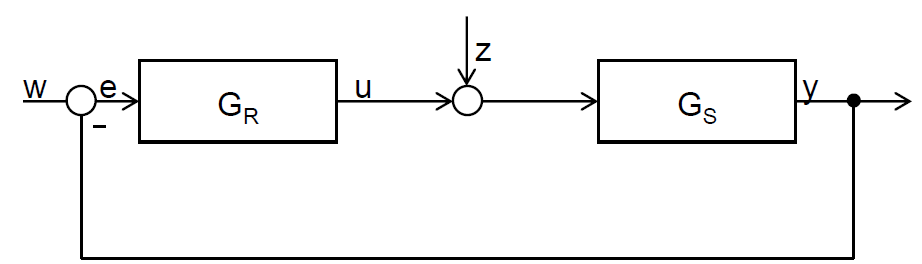
\includegraphics[scale=0.45]{Bilder/Kapitel 6/Standardregelkreis.PNG}
    \caption{Standardregelkreis}
    \label{fig:Abbildung4.1}
\end{figure}

%Chris
\subsection{Unterer Teillastbereich}

Laut \autoref{tab:Tabelle4.1} ist für den unteren Teillastbereich eine Leistungsoptimierung notwendig, da die Windleistung \acs{PW} unterhalb der Generatornennleistung \acs{PGNenn} liegt. Die Rotordrehzahl \acs{nR} liegt folglich noch unter der Generatornenndrehzahl \acs{nGNenn}, wodurch diese noch variabel an die Windgeschwindigkeit \acs{v1} angepasst werden kann. Dies wird mithilfe des bremsend wirkenden Generatormomentes \acs{MG} erreicht. Aufgrund dessen ergibt sich ein optimales Anströmverhältnis und es resultiert ein maximaler Leistungsbeiwert. Im unteren Teillastbereich kann mit steigender Windgeschwindigkeit also die maximal mögliche Windleistung entnommen werden, das heißt, der Leistungsbeiwert \acs{cP} wird stets auf den maximalen Leistungsbeiwert \acs{cPmax} geregelt.
\\
Für die Herleitung des Regelkreises wird von einer nicht linearen Bewegungs-DGL des torsionsstarren Triebstrangs ausgegangen. Der Vorteil für die Reglerauslegung im unteren Teillastbereich besteht darin, dass von der nicht linearen Bewegungs-DGL aus einer Leistungsbilanz ein Regelgesetz abgeleitet wird, welches einen Zusammenhang zwischen Regel- und Stellgröße darstellt. Durch das Regelgesetz wird mithilfe des berechneten Generatormoments \acs{MG} eine stationäre Rotordrehzahl \acs{omegaR} eingestellt. Es wird für diese Methode keine Führungsgröße benötigt. Dies vereinfacht die Entwicklung des Regelkreises für den unteren Teillastbereichs deutlich, da keine genaue Kenntnis der Steckenübertragungsfunktion nötig ist. Daher kann der untere Teillastbereich nicht als Standardregelkreis betrachtet werden. Dieses \glqq Steuerungskonzept\grqq{} zur Regelung des unteren Teillastbereiches hat sich als Standardmethode für diesen Arbeitsbereich durchgesetzt. Das Regelgesetz für die Stellgröße \acs{MG} wird mit folgenden Gleichungen beschrieben:

\begin{align}
    \acs{MG}(\acs{omegaG}) = k_I \cdot \acs{omegaR}^2 \enspace ,wobei \enspace \acs{kI} = const.
    \label{eq:Gleichung4.1}
\end{align}

mit:

\begin{align}
   \acs{kI} = \frac{1}{2} \cdot \rho \cdot \pi \cdot R^5 \cdot \frac{1}{\acs{lambdaopt}^3} \cdot \frac{1}{\acs{ng}} \cdot \acs{cP}(\acs{lambdaopt})
   \label{eq:Gleichung4.2}
\end{align}
\newline
Der Vorteil bei diesem Steuerungskonzept besteht nun darin, dass für jede Änderung der Windgeschwindigkeit \acs{v1} ein neuer stationärer Arbeitspunkt mit stationärer Rotorwinkelgeschwindigkeit \acs{omegaR} entsteht. Dabei ergibt sich ein entsprechendes Generatormoment \acs{MG}, welches mithilfe der \autoref{eq:Gleichung4.1} und \autoref{eq:Gleichung4.2} berechnet wird. Das heißt, zu jeder Windgeschwindigkeit wird das zugehörige Generatormoment \acs{MG} zugeordnet, wodurch die Notwendigkeit eines PI(D)-Reglers entfällt.
\\
Die Rotorwinkelgeschwindigkeit \acs{omegaR} wird stets optimal an die Windgeschwindigkeit angepasst. Es besteht für stationäre Arbeitspunkte ein eindeutiger Zusammenhang zwischen Rotordrehzahl \acs{omegaR} und der Windgeschwindigkeit \acs{v1}. Die optimale Schnelllaufzahl \acs{lambdaopt} kann im voraus berechnet werden und ist für den unteren Teillastbereich konstant. Aufgrund dessen, wird mithilfe der \autoref{eq:Gleichung4.3}, aus der Rotorwinkelgeschwindigkeit und konstanten Schnelllaufzahl die zugehörige Windgeschwindigkeit \acs{v1} berechnet.  Damit ergibt sich für den Leistungsbeiwert \acs{cP} ein optimaler Leistungsbeiwert \acs{cPopt}, jedoch für den Momentenbeiwert \acs{cM} kein optimaler Momentenbeiwert \acs{cMopt}. Aus der Formulierung der Regelziele ergab sich eine Leistungsoptimierung für den unteren Teillastbereich, sodass der Leistungsbeiwert \acs{cP} auf einen optimalen Wert geregelt werden muss, da erst so die maximale Entnahme der Windleistung \acs{PW} entsteht. Daher wird das Erreichen eines optimalen Momentenbeiwertes \acs{cMopt} nicht angestrebt, da die Leistungsoptimierung durch Drehzahlanpassung stattfindet.   

\begin{align}
    \acs{v1} = \frac{\acs{omegaR} \cdot {R}}{\acs{lambdaopt}} \enspace ,wobei \enspace \acs{lambda} = \acs{lambdaopt}
    \label{eq:Gleichung4.3}
\end{align}
\newline
Die Steuerung für den unteren Teillastbereich wird als Funktionsblock in Matlab Simulink implementiert. In diesem Block wird der Faktor \acs{kI} berechnet und hinterher mit der Rotorwinkelgeschwindigkeit $\acs{omegaR}^2$ multipliziert, um als Ergebnis eine Generatormomentsollwertvorgabe $M_{G,soll}$ für das Triebstrangmodell zu erhalten. Die \autoref{fig:Abbildung4.2} zeigt die Blockdarstellung der Steuerung inklusive der Ein- und Ausgansparameter.

\newpage

\begin{figure}[H]
   \centering
   \begin{pspicture}[showgrid=false](0,0)(10,5)
        \psframe(0,0)(10,5)
        % Modell
        \psframe[linecolor=black,fillcolor=lightGrey,fillstyle=solid](0.5,0.5)(4,4.5)
        \rput(2.25,2.8){\small Steuerung unterer}
        \rput(2.25,2.3){\small Teillastbereich}
        % Ausgänge Block
        \psline{->}(4,2.5)(6,2.5)
        \rput(5.5,2.9){\footnotesize \acs{kI}}
        %Multiplikation
        \psframe[linecolor=black,fillcolor=lightGrey,fillstyle=solid](6.0,0.5)(6.5,4.5)
        \rput(6.25,2.5){\small \cdot}
        % Eingang Multiplikation
        \psline{-}(4.5,4.5)(4.5,3.5)
        \psline{->}(4.5,3.5)(6,3.5)
        \rput(5.3,4.5){\footnotesize {\acs{omegaR}$^2$}}
        % Ausgang Multiplikation
        \psline{->}(6.5,2.5)(9,2.5)
        \rput(8.5,2.9){\footnotesize \acs{MG}}
    \end{pspicture}
   \caption[Übersicht Steuerung unterer Teillastbereich]{Blockdarstellung der Steuerung des unteren Teillastbereichs inklusive der Ein- und Ausgangsparameter}
   \label{fig:Abbildung4.2}
\end{figure}

%Chris
\subsection{Linearisierung der Streckenübertragungsfunktion}
Für die Reglerauslegung im oberen Teillastbereich und Vollastbereich müssen zunächst die Streckenübertragungsfunktionen ausgehend vom torsionsstarren Antriebstrangmodell und der daraus resultierenden nichtlinearen Bewegungs-DGL linearisiert werden. Aus dem Ergebnis der Linearisierung entstehen sogenannte Linearisierungskoeffizienten, welche für bestimmte stationäre Arbeitspunkte zugeordnet sind. Für den oberen Teillastbereich und dem Volllastbereich werden zunächst jeweils drei stationäre Arbeitspunkte mit den entsprechenden Linearisierungskoeffizienten betrachtet. Die Linearisierung erfolgt mittels der Taylorreihenentwicklung. Aus dem Funktionsmodell ergibt sich mit \autoref{eq:Gleichung4.4} die nichtlineare Bewegugns-DGL des Antriebstrangs, welche bereits im Kapitel 3 ausführlich diskutiert wurde. 

\begin{align}
    \ddot\varphi_R = \frac{1}{J} \cdot (\acs{MR} - \acs{ng} \cdot \acs{MG})
    \label{eq:Gleichung4.4}
\end{align}
\newline
Mithilfe der Taylorreihenentwicklung um einen stationären Arbeitspunkt \acs{omegaR} und lösen der nichtlinearen Bewegungs-DGL mit der Laplacetransformation ergibt sich folgende \autoref{eq:Gleichung4.5}, wobei sich insgesamt vier Linearisierungskoeffizienten ergeben, bei dem der Koeffizient bezogen auf das Generatormoment \acs{MG} nicht benötigt wird und daher nicht weiter aufgeführt ist.
\begin{align}
    \acs{omegaR} &= \frac{1}{J \cdot s - k_{\omega\mathrm{R}}} \cdot (\acs{kv} \cdot v + \acs{ktheta} \cdot \theta - \acs{ng} \cdot \acs{MG})\label{eq:Gleichung4.5}
    \enspace,wobei\\
    k_{\omega\mathrm{R}} &:= \left(\frac{\delta \acs{MR}}{\delta v}\right)_c , \enspace \acs{kv} := \left(\frac{\delta \acs{MR}}{\delta \omega_{\mathrm{R}}}\right)_c, \enspace  \acs{ktheta} := \left(\frac{\delta \acs{MR}}{\delta \theta}\right)_c  \nonumber
\end{align}
\newline
Zur Berechnung der Linearisierungskoeffizienten muss nun die Berechnungsvorschrift für das Rotormoment \acs{MR} aus \autoref{eq:Gleichung2.39} partiell abgeleitet werden, wobei der Momentenbeiwert \acs{cM} ebenfalls partiell nach \acs{lambda} und $\theta$ abgeleitet werden muss. Daraus ergeben sich die folgenden Gleichungen.

\begin{align}
    k_{\omega\mathrm{R,II(I),i}} &\approx \left(\frac{1}{2} \cdot \rho \cdot \acs{v1}^2 \cdot \pi \cdot \acs{R}^3 \cdot \left(\frac{\acs{R}}{\acs{v1}} \cdot \frac{\delta \acs{cM}_{,II(I),i}\left(\acs{lambda}\left(v,\acs{omegaR}\right),\theta\right)}{\delta \acs{lambda}}\right)\right)_c\label{eq:Gleichung4.6}\\
     \acs{kv}_{,II(I),i} &\approx \left(\frac{1}{2} \cdot \rho \cdot \acs{v1}^2 \cdot \pi \cdot \acs{R}^3 \cdot \left(2 \cdot \acs{v1} \cdot \acs{cM}_{,II(I),i}\left(\acs{lambda}\left(v,\acs{omegaR}\right),\theta\right) - \acs{omegaR} \cdot \acs{R} \cdot \frac{\delta \acs{cM}_{,II(I),i}\left(\acs{lambda}\left(v,\acs{omegaR}\right),\theta\right)}{\delta \acs{lambda}}\right)\right)_c\label{eq:Gleichung4.7}\\
    \acs{ktheta}_{,III,i} &\approx \left(\frac{1}{2} \cdot \rho \cdot \acs{v1}^2 \cdot \pi \cdot \acs{R}^3 \cdot \left(\frac{\delta \acs{cM}_{,III,i}\left(\acs{lambda}\left(v,\acs{omegaR}\right),\theta\right)}{\delta \acs{lambda}}\right)\right)_c\label{eq:Gleichung4.8}
\end{align}
\newline
Im Folgenden werden die weiteren nötigen Schritte aufgeführt, um die Berechnung der Linearisierungskoeffizienten zu vervollständigen. Zunächst berechnen sich die zugehörigen Schnelllaufzahlen \acs{lambda} für die Arbeitsbereiche und dessen stationäre Arbeitspunkte mit der \autoref{eq:Gleichung4.9}.

\begin{align}
    \acs{lambda}_{,II(I),i} = \frac{\acs{omegaR} \cdot R}{\acs{v1}_{,II(I),i}}
    \label{eq:Gleichung4.9}
\end{align}
\newline
Hinterher werden die partiellen Ableitungen der Momentenbeiwerte \acs{cM} mithilfe der \autoref{eq:Gleichung4.10} und Unterscheidung der Arbeitsbereiche berechnet. Für den oberen Teillastbereich muss die partielle Ableitung nach $\theta$ nicht erfolgen, da der Pitchwinkel hier Null beträgt. Der Pitchwinkel wird erst beim Volllastbereich von Bedeutung sein, wenn es darauf ankommt, die Rotordrehzahl \acs{nR} mithilfe des Pitchwinkels zu begrenzen.
\begin{align}
    \acs{cM}(\acs{lambda})_{,II(I),i,\theta} &= c_1 \cdot (1 + c_2 \cdot \sqrt{\theta + c_3}) + \frac{c_4}{\acs{lambda}}   \cdot (c_5 \cdot \acs{lambda}_i - c_6 \cdot \theta - c_7 \cdot \theta^{c_8} - c_9) \cdot e^{-c_{10} \cdot \acs{lambda}_i}
    \label{eq:Gleichung4.10}\\\enspace ,mit\nonumber\\
    \acs{lambda}_i &= \frac{1}{\acs{lambda}_{,II(I),i} + 0,008 \cdot \theta} - \frac{0,035}{c_{11} + c_{12} \cdot \theta^3}
    \nonumber
\end{align}

{\renewcommand{\arraystretch}{2}%
\begin{table}[H]
    \centering
    \begin{tabular}{|c|c|c|c|}
        \hline
        c$_1$ = 0,005 & c$_2$ = 1,53 & c$_3$ = 0,5 & c$_4$ = 0,18\\\hline
        c$_5$ = 121 & c$_6$ = 27,9 & c$_7$ = 198 & c$_8$ = 2,36\\\hline
        c$_9$ = 5,74& c$_{10}$ = 11,35 & c$_{11}$ = 16,1 & c$_{12}$ = 201\\\hline
    \end{tabular}
\end{table}
}

Die Berechnung der Schnelllaufzahlen \acs{lambda}$_{,II(I),i}$ für den jeweiligen Arbeitsbereich und dessen stationären Arbeitspunkte, die Berechnung der partiellen Ableitungen für die Momentenbeiwerte \acs{cM}$_{,II(I),i}$, sowie die Berechnung der Linearisierungskoeffizienten und dessen partielle Ableitungen, finden in einem separaten Matlab-File statt und werden bevor die Simulation gestartet wird vorangehend einmalig für die stationären Arbeitspunkte berechnet und für die Berechnung der Reglerkoeffizienten für den oberen Teillastbereich und Volllastbereich zur Verfügung gestellt, welche ebenfalls vor Simulationsstart einmalig berechnet werden und hinterher als Array der Simulation übergeben und in entsprechende Lookup Tables gespeichert werden.

%chris + Aaron
\subsection{Oberer Teillastbereich}
Laut \autoref{tab:Tabelle4.1} ist für den oberen Teillastbereich ebenfalls eine Leistungsoptimierung notwendig, da die Windleistung \acs{PW} noch unterhalb oder gleich der Generatornennleistung \acs{PGNenn} ist. Sofern die Rotordrehzahl \acs{nR} gleich der Generatornenndrehzahl \acs{nGNenn} ist, ist es nicht mehr möglich diese an die Windgeschwindigkeit anzupassen. Dadurch ergibt sich ein schlechtes Anströmverhältnis was einen nicht optimalen Leistungsbeiwert \acs{cP} zur Folge hat. Es wird zwar nicht mehr das Leistungsmaximum aus der zur Verfügung stehenden Windleistung entnommen, dennoch wird eine Leistungssteigerung mit ansteigender Windgeschwindigkeit \acs{v1} durch eine geeignete Regelung erzielt.\\
Für die Reglerauslegung des oberen Teillastbereiches wird eine algebraische Auslegung im Frequenzbereich durchgeführt. Zur Erfüllung der Hauptziele werden nun sogenannte Reglerkoeffizienten aus den vorher berechneten Linearisierungskoeffizienten ermittelt, welche später eine Generatormomentsollwertvorgabe $M_{G,soll}$ für den Antriebsstrang darstellen. Zur Bestimmung der Reglerkoeffizienten wird ein Referenzmodell herangezogen, welches das zu erwartendene Systemverhalten der Hauptziele des Reglers widerspiegelt. Dieses Referenzmodell wird anschließend mit dem physikalischen Modell, basierend auf den physikalischen Vorbetrachtungen der WEA, verglichen und überprüft, ob das gewünschte und resultierende Modell das gleiche Systemverhalten aufweist. Dieses Verfahren ist für das Führungs- und Störverhalten anzuwenden, wobei für den weiteren Verlauf der Arbeit sich auf das Führungsverhalten des Systems fokussiert wird. Auf Grundlage dessen, wird mittels Koeffizientenvergleich die Reglerkoeffizienten algebraisch berechnet. Auf die Herleitungen soll nicht weiter eingegangen werden. Damit ergibt sich für die Berechnung der Reglerkoeffizienten im oberen Teillastbereich folgende Gleichungen:
\begin{align}
    k_{P,W,II} &= \frac{3 \cdot J}{T_{Aus} \cdot i_G}   \label{eq:Gleichung4.11}\\
    k_{I,W,II} &= \frac{3 \cdot k_{\omega\mathrm{R,II,i}}}{T_{Aus} \cdot i_G}\label{eq:Gleichung4.12}
\end{align}
\newline
In Matlab werden nun die Reglerkoeffizienten einmalig für jeden Arbeitspunkt im oberen Teillastbereich berechnet und der Simulation als Lookup-Table übergeben. Da es sich hierbei um einen Delta-Regler handelt, muss die Differenz aus Soll-Drehzahl und Ist-Drehzahl mit den Reglerkoeffizienten verrechnet werden. Die Auswahl der richtigen Reglerkoeffizienten im Lookup-Table wird durch das entsprechende Generatormoment \acs{MG} im jeweiligen Arbeitspunkt bestimmt. Der Regelkreis für den oberen Teillastbereich ist grundlegend der \autoref{fig:Abbildung4.3} zu entnehmen.

 \begin{figure}[H]
    \centering
    \fbox{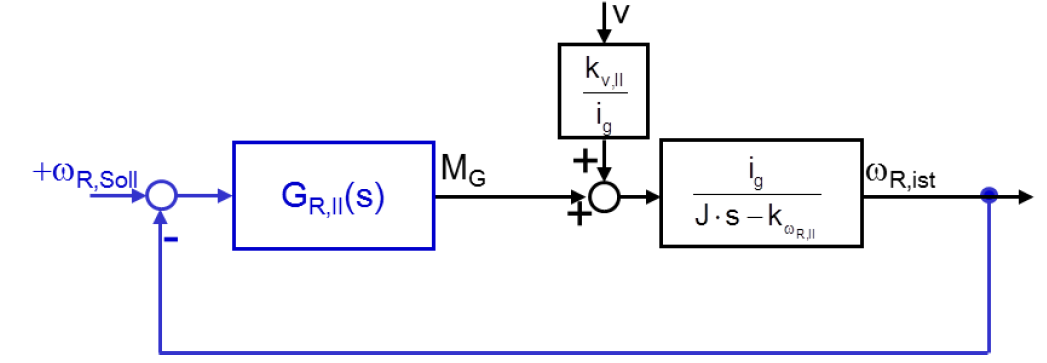
\includegraphics[width=0.9\textwidth]{Bilder/Kapitel 5/Führungsübertragungsfunktion_oberer_Teillastbereich.PNG}}
    \caption[Reglerkreis - oberer Teillastbereich]{Regelkreis - oberer Teillastbereich mit der Führungsübertragungsfunktion $G_{R,II}(s)$ \cite{SkriptSchulte}}
    \label{fig:Abbildung4.3}
\end{figure}

\subsection{Volllastbereich}
Laut \autoref{tab:Tabelle4.1} ist für den Volllastbereich eine Leistungsbegrenzung vorzusehen, da nun die Windleistung \acs{PW} oberhalb der Generatornennleistung \acs{PGNenn} liegt. Durch das Pitchen der Blätter wird bewusst das Anströmverhältnis verschlechtert, denn das Betreiben der WEA darf nicht weit über Nenndrehzahl erfolgen. Dies führt zur Beschädigung oder gar Zerstörung der WEA. Das Pitchen ermöglicht jedoch bei ansteigender Windleistung (\acs{PW} > \acs{PGNenn}) weiterhin eine konstante Generatornennleistung \acs{PGNenn} zu erzielen. Der Pitchwinkel \acs{theta} spielt nun für die Reglerauslegung eine entscheidene Rolle.\\
Das Vorgehen zur Bestimmung der Reglerkoeffizienten ist gleich dem Vorgehen aus dem oberen Teillastbereich. Das Verfahren ist hier ebenfalls auf das Führungs- und Störverhalten anzuwenden, jedoch wird beim Volllastbereich lediglich das Führungsverhalten betrachet. Die folgenden Gleichungen zeigen die Berechnungen der entsprechenden Reglerkoeffizienten. Der Unterschied hier ist, das der P- und I-Anteil des Reglers von $k_\theta$ abhängig ist. Im Volllastbereich gilt es den Pitchwinkel so zu regeln, dass das Generatormoment \acs{MG} = const. bleibt.

\begin{align}
    k_{P,W,III} &= \frac{3 \cdot J}{T_{Aus} \cdot k_\theta}   \label{eq:Gleichung4.13}\\
    \nonumber\\
    k_{I,W,III} &= \frac{3 \cdot k_{\omega\mathrm{R,III,i}}}{T_{Aus} \cdot k_\theta}\label{eq:Gleichung4.14}
\end{align}
\newline
Auch hier werden die Reglerkoeffizienten einmalig für jeden stationären Arbeitspunkt berechnet und der Simulation als Lookup-Table übergeben. Die Funktionsweise und Vorgehensweise ist dabei die Gleiche, wie beim oberen Teillastbereich, wobei die Auswahl der Reglerkoeffizienten anhand des einzustellenden Pitchwinkels erfolgt. Die \autoref{fig:Abbildung4.4} zeigt den grundlegenden Aufbau des Regelkreises für den Volllastbereich.

\begin{figure}[H]
    \centering
    \fbox{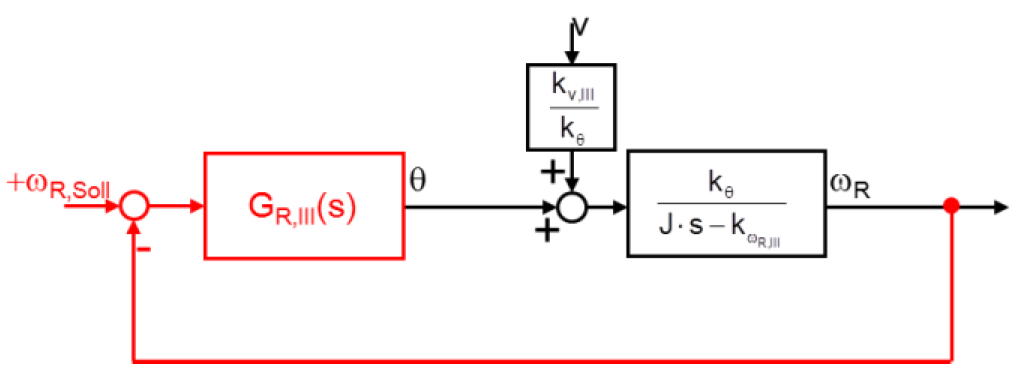
\includegraphics[width=0.9\textwidth]{Bilder/Kapitel 5/Führungsübertragungsfunktion_Volllastbereich.PNG}}
    \caption[Reglerkreis - Volllastbereich]{Regelkreis - Volllastbereich mit der Führungsübertragungsfunktion $G_{R,III}(s)$ \cite{SkriptSchulte}}
    \label{fig:Abbildung4.4}
\end{figure}

%Aaron
\subsection{Zustandsautomat} \label{statemachine}

Wie bereits in \autoref{regelziel} erläutert wurde, wird die Windenergieanlage in Abhängigkeit von der Windgeschwindigkeit \acs{v1} \bzw der Rotorwinkelgeschwindigkeit \acs{omegaR} in verschiedenen Lastbereichen mit ihren eigenen Regelzielen geregelt. Der Betrieb und damit auch die Regelung der Gesamtanlage bedarf folglich der Integration der in den vorangegangenen Unterabschnitten entworfenen Regler in eine Gesamtstruktur. \autoref{fig:Abbildung4.5} zeigt auf der linken Seite die Steuereinheit des unteren Teillastbereiches sowie die PI-Regler für den oberen- und den Volllastbereich. Da insbesondere die Regler nur für ihren jeweiligen Arbeitsbereich ausgelegt sind, ist es erforderlich deren Integratoren zurückzusetzen, wenn ein Lastbereich verlassen wird. Ebenfalls bedarf es einer Implementierung einer Sicherheitsabschaltung bei zu großen Windgeschwindigkeiten. Beide Aufgaben werden von einem Zustandsautomaten erfüllt, welcher in Simulink als Function-Block über die Nutzung einer Switch-Case-Anweisung implementiert wurde. Besagter Zustandsautomat ist in \autoref{fig:Abbildung4.5} auf der rechten Seite zu erkennen. Der Zustandsautomat erhält die Regelgrößen \acs{MG} für die beiden Teillastbereiche und \acs{theta} für den Vollastbereich, sowie die Ist-Winkelgeschwindigkeit des Rotors \acs{omegaRist} und die aktuelle Windgeschwindigkeit \acs{v1}. Von dem Zustandsautomaten werden die Sollwerte für \acs{MG} \bzw \acs{theta} und die Rücksetzbedingungen der beiden Integratoren in den PI-Reglern ausgegeben. 

\begin{figure}[H]
   \centering
   \begin{pspicture}[showgrid=false](0,0)(12,9.5)
        \psframe(0,0)(12,9.5)
        % UTLB
        \psframe[linecolor=black,fillcolor=lightGrey,fillstyle=solid](0.5,0.5)(4.5,2.5)
        \rput(2.5,1.75){\small Regler}
        \rput(2.5,1.25){\small Volllastbereich}
        % OTLB
        \psframe[linecolor=black,fillcolor=lightGrey,fillstyle=solid](0.5,3)(4.5,5)
        \rput(2.5,4.25){\small Regler oberer}
        \rput(2.5,3.75){\small Teillastbereich}
        % VLB
        \psframe[linecolor=black,fillcolor=lightGrey,fillstyle=solid](0.5,5.5)(4.5,7.5)
        \rput(2.5,6.75){\small Steuerung unterer}
        \rput(2.5,6.25){\small Teillastbereich}
        % Statemachine
        \psframe[linecolor=black,fillcolor=lightGrey,fillstyle=solid](6.5,0.5)(10,9)
        \rput(8.25,5.25){\small Zustands-}
        \rput(8.25,4.75){\small automat}
        % Regler -> Statemachine
        \psline{->}(4.5,1.5)(6.5,1.5)
        \rput(5.5,1.8){\footnotesize \acs{theta3}}
        \psline{->}(4.5,4)(6.5,4)
        \rput(5.5,4.3){\footnotesize \acs{MG2}}
        \psline{->}(4.5,6.5)(6.5,6.5)
        \rput(5.5,6.8){\footnotesize \acs{MG1}}
        % -> Statemachine
        \psline{-}(5.5,9)(5.5,8.5)
        \psline{->}(5.5,8.5)(6.5,8.5)
        \rput(5.2,8.75){\footnotesize \acs{v1}}
        \psline{->}(2.5,8)(6.5,8)
        \rput(3.5,8.3){\footnotesize \acs{omegaRist}}
        % Statemachine ->
        \psline{->}(10,8)(11.5,8)
        \rput(10.75,8.3){\footnotesize \acs{MGsoll}}
        \psline{->}(10,5.827)(11.5,5.827)
        \rput(10.75,6.127){\footnotesize \acs{thetasoll}}
        \psline{->}(10,3.66)(11.5,3.66)
        \rput(10.75,3.96){\footnotesize $Reset_{\mathrm{II}}$}
        \psline{->}(10,1.5)(11.5,1.5)
        \rput(10.75,1.8){\footnotesize $Reset_{\mathrm{III}}$}
    \end{pspicture}
   \caption[Regeleinheit der WEA]{Blockdarstellung der Regeleinheit der Windenergieanlage inklusive des Zustandsautomaten und der Regler für die drei Lastbereiche}
   \label{fig:Abbildung4.5}
\end{figure}

\autoref{fig:Abbildung4.6} zeigt das Zustandsdiagramm, welches in Simulink umgesetzt wurde. Gut im mittleren Bereich der Abbildung zu erkennen, sind die von \acs{omegaRist} abhängigen Übergangsbedingungen zwischen den Lastbereichen. Von entscheidender Relevanz für die Verhinderung der Zerstörung der WEA ist die Abschaltbedingung bei zu großen Winden ($v_1 > v_{\mathrm{1,krit}} = \SI{25}{\frac{m}{s}}$), welche in jedem Zustand berücksichtigt wird.

\begin{figure}[H]
    \centering
    \begin{pspicture}[showgrid=false](0,0)(15,18)
        \psframe(0,0)(15,18)
        
        % STATES
        % Idle State
        \Cnode[fillstyle=solid,fillcolor=lightGrey,radius=1cm](7.5,15.5){A}
        \rput(A){Idle}
        % UTLB
        \Cnode[fillstyle=solid,fillcolor=lightGrey,radius=1cm](12.5,11.5){B}
        \rput(B){UTLB $\mathrm{I}$}
        % OTLB
        \Cnode[fillstyle=solid,fillcolor=lightGrey,radius=1cm](7.5,7.5){C}
        \rput(C){OTLB $\mathrm{II}$}
        % VLB
        \Cnode[fillstyle=solid,fillcolor=lightGrey,radius=1cm](2.5,11.5){D}
        \rput(D){VLB $\mathrm{III}$}
        % E-Stop
        \Cnode[fillstyle=solid,fillcolor=lightGrey,radius=1cm](7.5,2.5){E}
        \rput(E){E-Stop}
        
        % VERBINDUNGEN
        % Start
        \psline{->}(5,15.5)(6.51,15.5)
        \rput*(5.5,15.8){\small$Start$}
        % Idle -> Idle
        \ncloop[angleB=105, angleA=75, loopsize=0, arm=0.5, linearc=0.2]{->}{A}{A}
        \ncput*{\small$else$}
        % Idle -> UTLB
        \nccurve[angleB=90, angleA=0]{->}{A}{B}
        \ncput*{\small$\omega_{\mathrm{r,ist}} \geq 0.3 \cdot \omega_{\mathrm{r,nenn}}$}
        % UTLB -> Idle
        \nccurve[angleB=-50, angleA=150]{->}{B}{A}
        \ncput*{\small$\omega_{\mathrm{r,ist}} < 0.25 \cdot \omega_{\mathrm{r,nenn}}$}
        % UTLB -> UTLB
        \ncloop[angleB=-15, angleA=15, loopsize=0, arm=0.5, linearc=0.2]{->}{B}{B}
        \ncput*{\small$else$}
        % UTLB -> OTLB
        \nccurve[angleB=0, angleA=-60]{->}{B}{C}
        \ncput*{\small$\omega_{\mathrm{r,ist}} \geq 0.9 \cdot \omega_{\mathrm{r,nenn}}$}
        % OTLB -> UTLB
        \nccurve[angleB=-120, angleA=30]{->}{C}{B}
        \ncput*{\small$\omega_{\mathrm{r,ist}} < 0.85 \cdot \omega_{\mathrm{r,nenn}}$}
        % OTLB -> OTLB
        \ncloop[angleB=-60, angleA=-30, loopsize=-0.4, arm=0.5, linearc=0.2]{->}{C}{C}
        \ncput*{\small$else$}
        % OTLB -> VLB
        \nccurve[angleB=70, angleA=60]{->}{C}{D}
        \ncput*{\small$\omega_{\mathrm{r,ist}} \geq \omega_{\mathrm{r,nenn}}$}
        % VLB -> OTLB
        \nccurve[angleB=120, angleA=0]{->}{D}{C}
        \ncput*{\small$\omega_{\mathrm{r,ist}} < 0.98 \cdot \omega_{\mathrm{r,nenn}}$}
        % VLB -> VLB
        \ncloop[angleB=165, angleA=195, loopsize=0, arm=0.5, linearc=0.2]{->}{D}{D}
        \ncput*{\small$else$}
        % UTLB -> E-Stop
        \nccurve[angleB=0, angleA=-45]{->}{B}{E}
        \ncput*{\small$v_1 > v_{1,\mathrm{krit}}$}
        % OTLB -> E-Stop
        \nccurve[angleB=90, angleA=-90]{->}{C}{E}
        \ncput*{\small$v_1 > v_{1,\mathrm{krit}}$}
        % VLB -> E-Stop
        \nccurve[angleB=180, angleA=-100]{->}{D}{E}
        \ncput*{\small$v_1 > v_{1,\mathrm{krit}}$}
        % Idle -> E-Stop
        \nccurve[angleB=130, angleA=-110]{->}{A}{E}
        \ncput*{\small$v_1 > v_{1,\mathrm{krit}}$}
        % E-Stop -> Idle
        \nccurve[angleB=-130, angleA=160]{->}{E}{A}
        \ncput*{\small$v_1 < 0.9 \cdot v_{1,\mathrm{krit}}$}
        % E-Stop -> E-Stop
        \ncloop[angleB=255, angleA=285, loopsize=0, arm=0.5, linearc=0.2]{->}{E}{E}
        \ncput*{\small$else$}
    \end{pspicture}
    \caption[Statemachine WEA]{Statemachine-Abbildung zur Darstellung der Lastbereiche und den jeweiligen Übergangsbedingungen}
    \label{fig:Abbildung4.6}
\end{figure}

%Aaron
\subsection{Reglervalidierung} \label{reglervalidierung}

Ziel dieses Unterabschnittes ist die Verifikation der erfolgreichen Umsetzung der Regelziele, die Funktionstüchtigkeit der Regler in Bezug auf die zuvor entwickelten Teilmodelle der Anlage und die Prüfung der Einhaltung der definierten Grenzen (Constraints) des Systems. Letztere können in \autoref{einfuehrung} nachgelesen werden. \\
Die Validierung der Regelung gliedert sich grundsätzlich in die Bereiche \glqq 4.7.1: Darstellung der Simulationsergebnisse\grqq{}, \glqq 4.7.2: Validierung der Regelziele\grqq{} und \glqq 4.7.3: Prüfung der Einhaltung der Constraints\grqq{}. Zunächst sollen generelle Zusammenhänge grafisch dargestellt und diskutiert werden. Daran anschließend wird geprüft, inwiefern sich die Ergebnisse mit den beschriebenen Regelzielen decken. Abschließend werden insbesondere die nicht eingehaltenen Grenzen des Systems auf ihre Ursache diskutiert. Im Ausblick (\autoref{ausblick}) werden mögliche Lösungsansätze für ermittelte Probleme kurz dargestellt.

\subsubsection{Darstellung der Simulationsergebnisse}

Das Modell der WEA inklusive der Steuerung/Regelung dieser wird gegen verschiedene Winde als Störgröße getestet. Auf die Prüfung des Führungsverhaltens wird an dieser Stelle verzichtet, da der Einfluss des Windes als Störgröße von größerer Bedeutung ist. Getestet werden soll das entwickelte System gegen:
\begin{enumerate}
    \item Winde mit konstanten Windgeschwindigkeiten
    \item Einzelne (IEC) Windböen
    \item Turbulente Winde
    \item Windgeschwindigkeitsstufen
\end{enumerate}

Dabei werden verschiedene Windgeschwindigkeiten beispielhaft simuliert. Begonnen werden soll mit dem Test des Modells gegen konstante Windgeschwindigkeiten. Windgeschwindigkeiten wurden hier so ausgewählt, dass die einzelnen Lastbereiche (Arbeitsbereiche) gut dargestellt werden können und Übergangsbedingungen klar zu erkennen sind.\\

\autoref{fig:Bild4.7} zeigt die Simulationsergebnisse für eine konstante Windgeschwindigkeit von $\SI{8}{\frac{m}{s}}$. In der oberen Abbildungshälfte dargestellt, werden die generatorseitige Winkelgeschwindigkeit und die Generatorleistung. An der Winkelgeschwindigkeit ist gut zu erkennen, dass durch die anliegende Windgeschwindigkeit der Rotor und damit auch der Generator beschleunigen, bis \ca zum Zeitpunkt \SI{90}{s} bei gegebenem Wind eine stationäre Geschwindigkeit erreicht wird. Die Winkelgeschwindigkeit stagniert bei rund einer Umdrehung pro Sekunde \bzw \SI{90}{\frac{rad}{s}}. Die Leistungskurve des Generators hat einen sehr ähnlichen Verlauf. Jedoch ist ein wesentlicher Unterschied im Bereich von $\SI{0}{s}$ bis $\SI{58}{s}$ zu erkennen. Erst ab $30\%$ der Nenndrehzahl des Rotors (vgl.\xspace \autoref{fig:Abbildung4.6} Zustand UTLB $\mathrm{I}$) setzt der untere Teillastbereich ein und damit auch die Ausgabe einer Leistung. Vorher befindet sich die Windenergieanlage noch im Leerlauf.

\begin{figure}[H]
   \centering
   \fbox{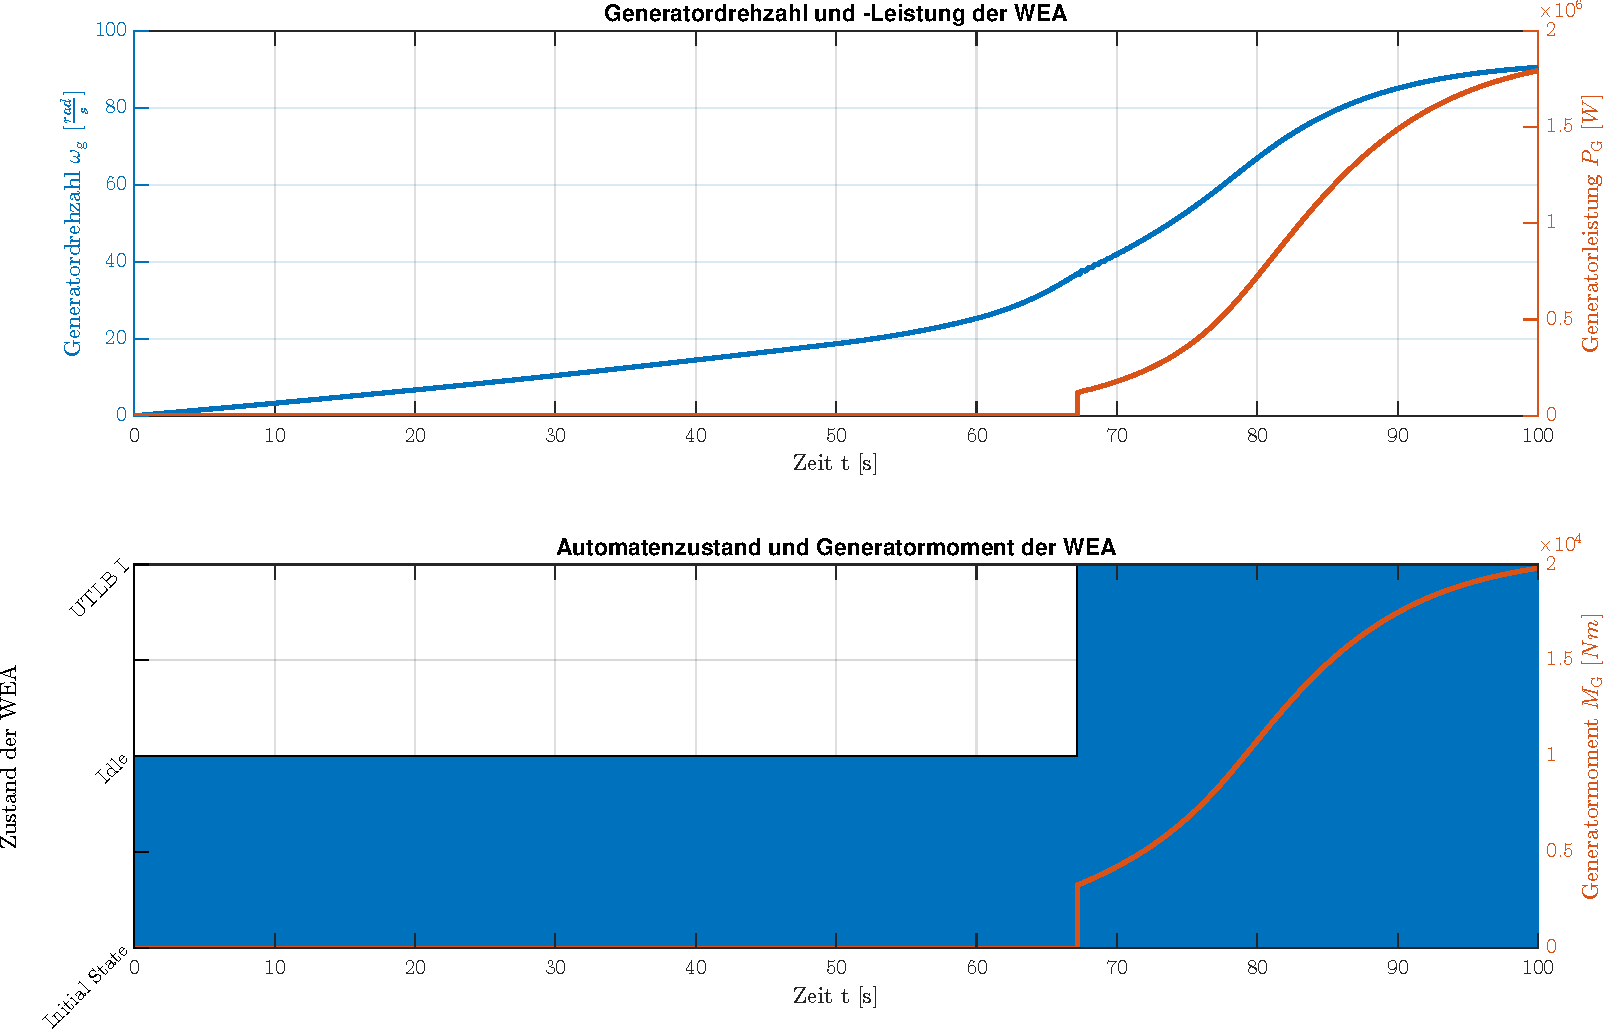
\includegraphics[width=1\textwidth]{Bilder/Kapitel 6/Reglervalidierung/const_wind_low.pdf}}
   \caption[Simulationsergebnisse langsamer konstanter Wind]{Simulationsergebnisse bei einem eingeprägten konstanten Wind von $\SI{9}{\frac{m}{s}}$}
   \label{fig:Bild4.7}
\end{figure}

In der unteren Hälfte von \autoref{fig:Bild4.7} zu erkennen ist der Zustand \bzw der Arbeitsbereich der Anlage sowie das generatorseitige Drehmoment. Da mit $\SI{9}{\frac{m}{s}}$ noch keine ausreichend hohe Rotordrehzahl erreicht wird, springt der Zustand lediglich vom Idle-Zustand in den unteren Teillastbereich. Ab dem Einsetzen des unteren Teillastbereiches liegt ein Moment am Generator an, welches aus dem rotorseitigen Moment resultiert. Auch das Moment steigt in einem ähnlichen Verlauf wie die Drehzahl an, bis zu dem Punkt, wo dem Wind die maximal mögliche Windleistung entnommen wird.\\

In \autoref{fig:Bild4.8} ist ein sehr ähnlicher Verlauf zu erkennen. In diesem Fall wurde mit einer Windgeschwindigkeit \acs{v1} von $\SI{10.7}{\frac{m}{s}}$ simuliert. In der oberen Hälfte ist die \ac{PG} und die Rotorwinkelgeschwindigkeit (\sim Rotordrehzahl) \ac{omegaG} erneut dargestellt. Die Leistung steigt nun bis knapp unter die Nennleistung an. Gleiches gilt auch für die Drehzahl. Die Leistung und das Generatordrehmoment setzen wie bereits zuvor bei $30\%$ der Nenndrehzahl ein.\\
Insbesondere ist in der unteren Hälfte der Abbildung die Einteilung der Kurven in die Last- \bzw Arbeitsbereiche ersichtlich. Bei \ca $\SI{69}{s}$ wird aufgrund des Erreichens von $90\%$ der Nenndrehzahl in den oberen Teillastbereich umgeschaltet. Die Umschaltbedingung geht aus \autoref{fig:Abbildung4.6} Zustand OTLB $\mathrm{II}$ hervor.

\begin{figure}[H]
   \centering
   \fbox{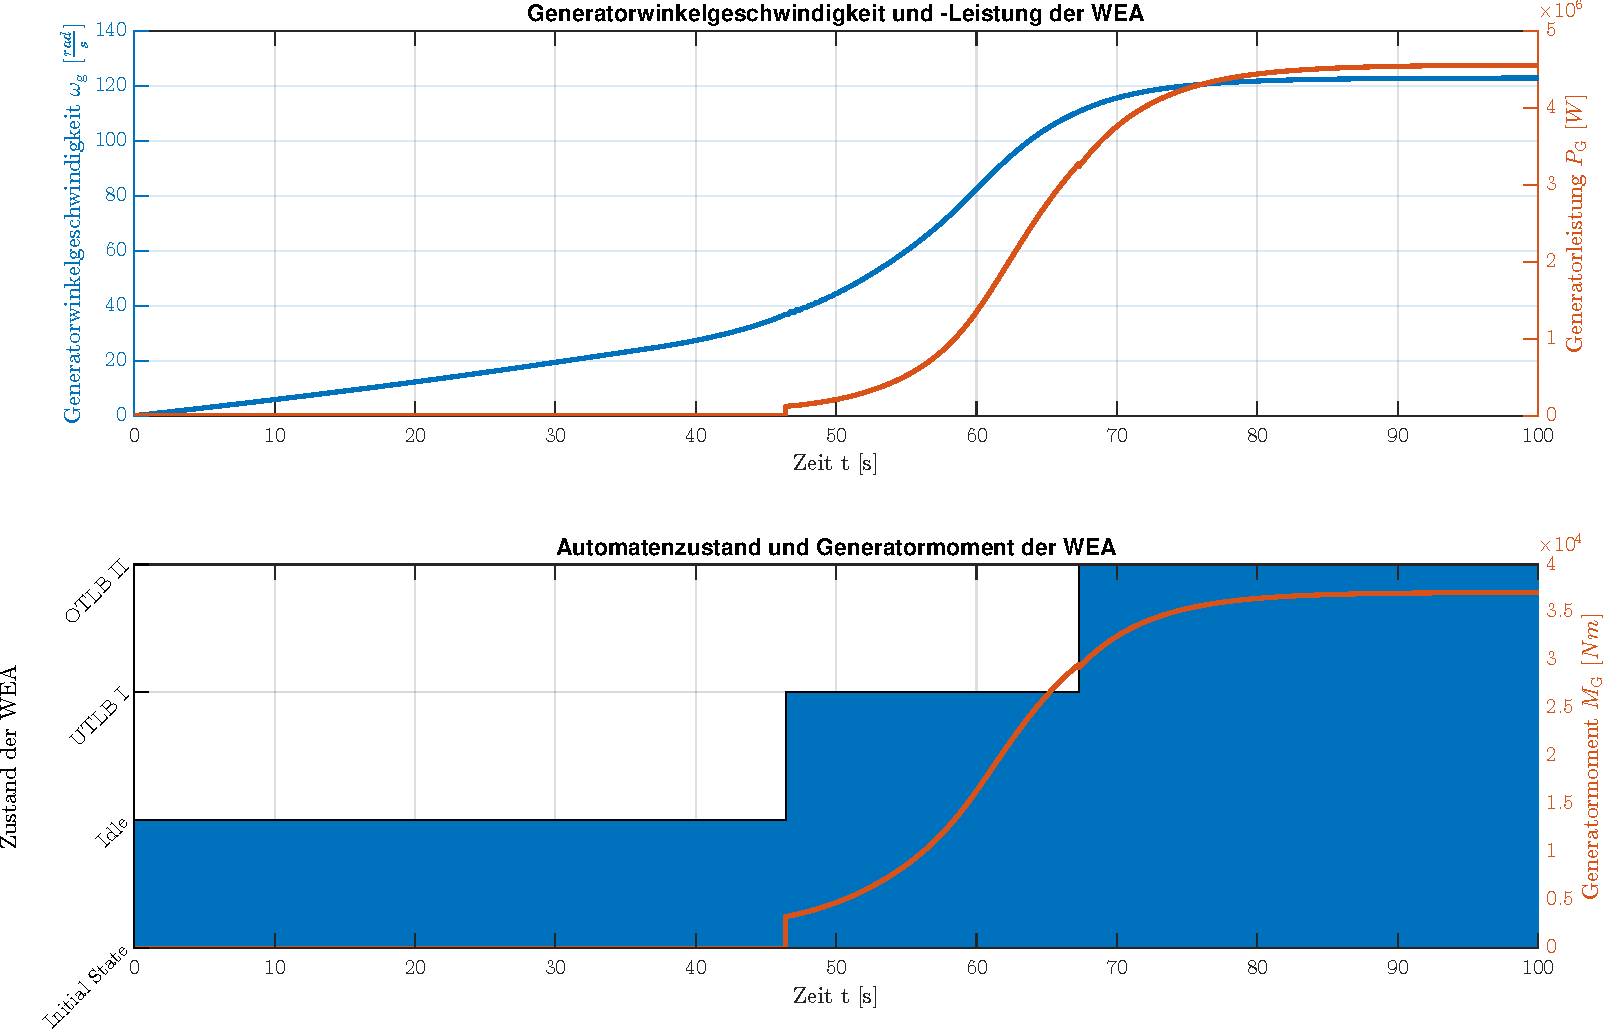
\includegraphics[width=1\textwidth]{Bilder/Kapitel 6/Reglervalidierung/const_wind_medium.pdf}}
   \caption[Simulationsergebnisse moderater konstanter Wind]{Simulationsergebnisse bei einem eingeprägten konstanten Wind von $\SI{10.7}{\frac{m}{s}}$}
   \label{fig:Bild4.8}
\end{figure}

Das letzte Diagramm aus der Reihe der konstanten Winde (\autoref{fig:Bild4.9}) bildet die Kurvenverläufe für einen Wind mit der Geschwindigkeit $\SI{14}{\frac{m}{s}}$ ab. Da der Wind nun stark genug ist, den Rotor bis zur Nenndrehzahl (und theoretisch auch darüber hinaus) zu beschleunigen, schaltet die Steuerung bis in den Volllastbereich hoch. Um die Nenngrößen für Drehzahl und Moment (\sim Leistung) konstant zu halten, müssen die Rotorblätter gepitched werden. Somit wurde ein weiterer Bereich in der Abbildung hinzugefügt, in welchem der \ac{theta} dargestellt wird.\\
Wenn man nun zunächst den oberen Teil der Grafik betrachtet, fällt auf, dass sowohl die Leistung als auch die Drehzahl leicht überschwingen, bevor sie auf dem Nennwert zurückfallen und nachfolgend konstant verlaufen. Grund dafür geht aus dem unteren Teil der Abbildung hervor. Der Pitchwinkel benötigt eine gewisse Zeit, bevor er seinen Sollwert erreicht hat. In dieser Zeit kommt es zu einer Überhöhung der Drehzahl und des Drehmoments auf der Rotorseite, welche wiederum auf die Generatorseite übertragen wird.\\
In der Mitte der Abbildung können erneut der aktuelle Arbeitsbereich und das Generatormoment abgelesen werden. Auch hier zeigt sich, dass bei \ca $\SI{51}{s}$ in den Vollastbereich umgeschaltet wird. Getriggert wird der Lastbereich durch das Erreichen der Nenndrehzahl (vgl.\xspace \autoref{fig:Abbildung4.6} Zustand VLB $\mathrm{III}$). Beim Generatormoment ist nun ebenfalls ein Unterschied zu den Teillastbereichen zu erkennen. Sobald die Nenndrehzahl erreicht wird, knickt das Moment sofort ab und verweilt konstant bei Nennmoment.\\
Der Pitchwinkel im unteren Bereich der Abbildung verweilt zunächst bis zum Umschalten in den Vollastbereich bei $0^\circ$. Erst dann steigt dieser mit $\SI{8}{\frac{^\circ}{s}}$ bis zum benötigten Pitchwinkel für die anliegende Windgeschwindigkeit an.

\begin{figure}[H]
   \centering
   \fbox{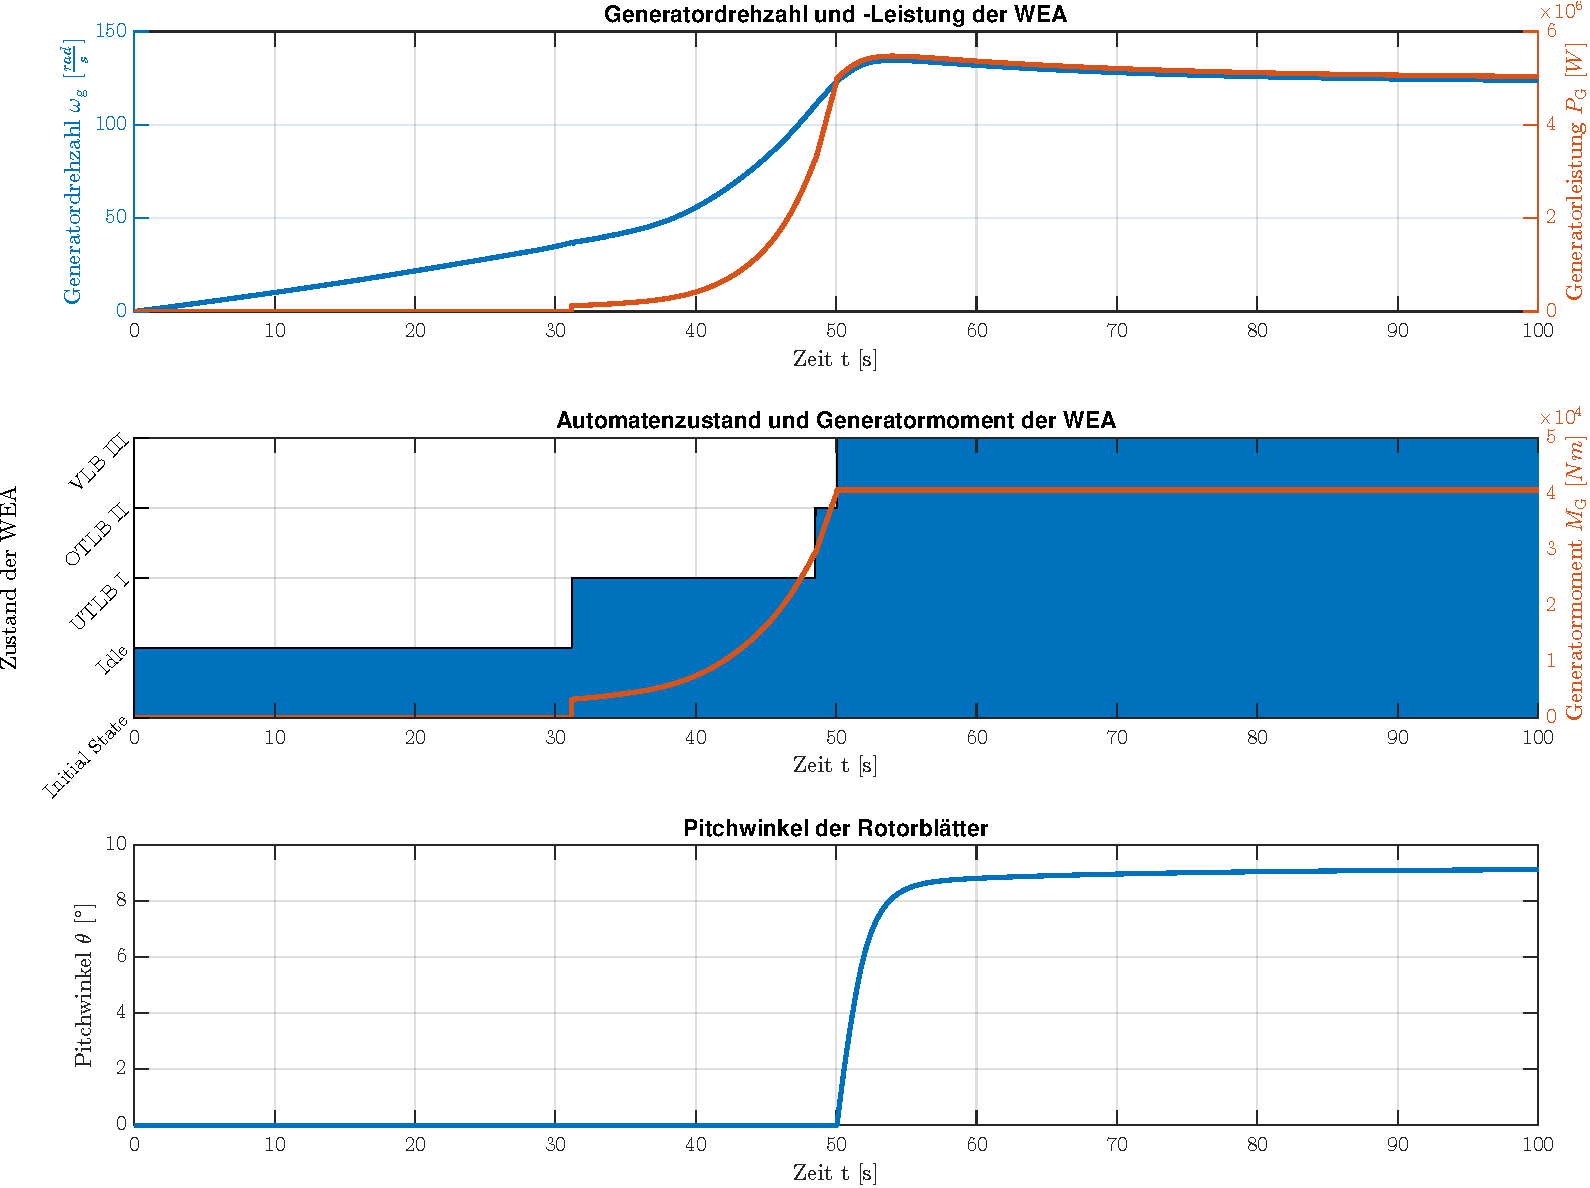
\includegraphics[width=1\textwidth]{Bilder/Kapitel 6/Reglervalidierung/const_wind_high.pdf}}
   \caption[Simulationsergebnisse schneller konstanter Wind]{Simulationsergebnisse bei einem eingeprägten konstanten Wind von $\SI{14}{\frac{m}{s}}$}
   \label{fig:Bild4.9}
\end{figure}

\autoref{fig:Bild4.10} zeigt einen Vergleich mehrerer Windgeschwindigkeiten in einem Diagramm. Dargestellt werden die Generatorwinkelgeschwindigkeit \acs{omegaG}, die Generatorleistung \acs{PG} und der Pitchwinkel \acs{theta}. Auf der linken Seite der Diagramme ist jeweils eine Legende mit den Windgeschwindigkeiten, bei welchen ein Kurvenverlauf entstanden ist.\\
Zunächst wird die Generatorwinkelgeschwindigkeit betrachtet. Es fällt auf, dass alle Kurven zwei Biegestellen besitzen. Bei der ersten vergrößert sich die Steigung und bei der zweiten sinkt sie. Je größer die eingeprägte Windgeschwindigkeit ist, desto schneller werden die beiden Stellen erreicht. 

\begin{figure}[H]
   \centering
   \fbox{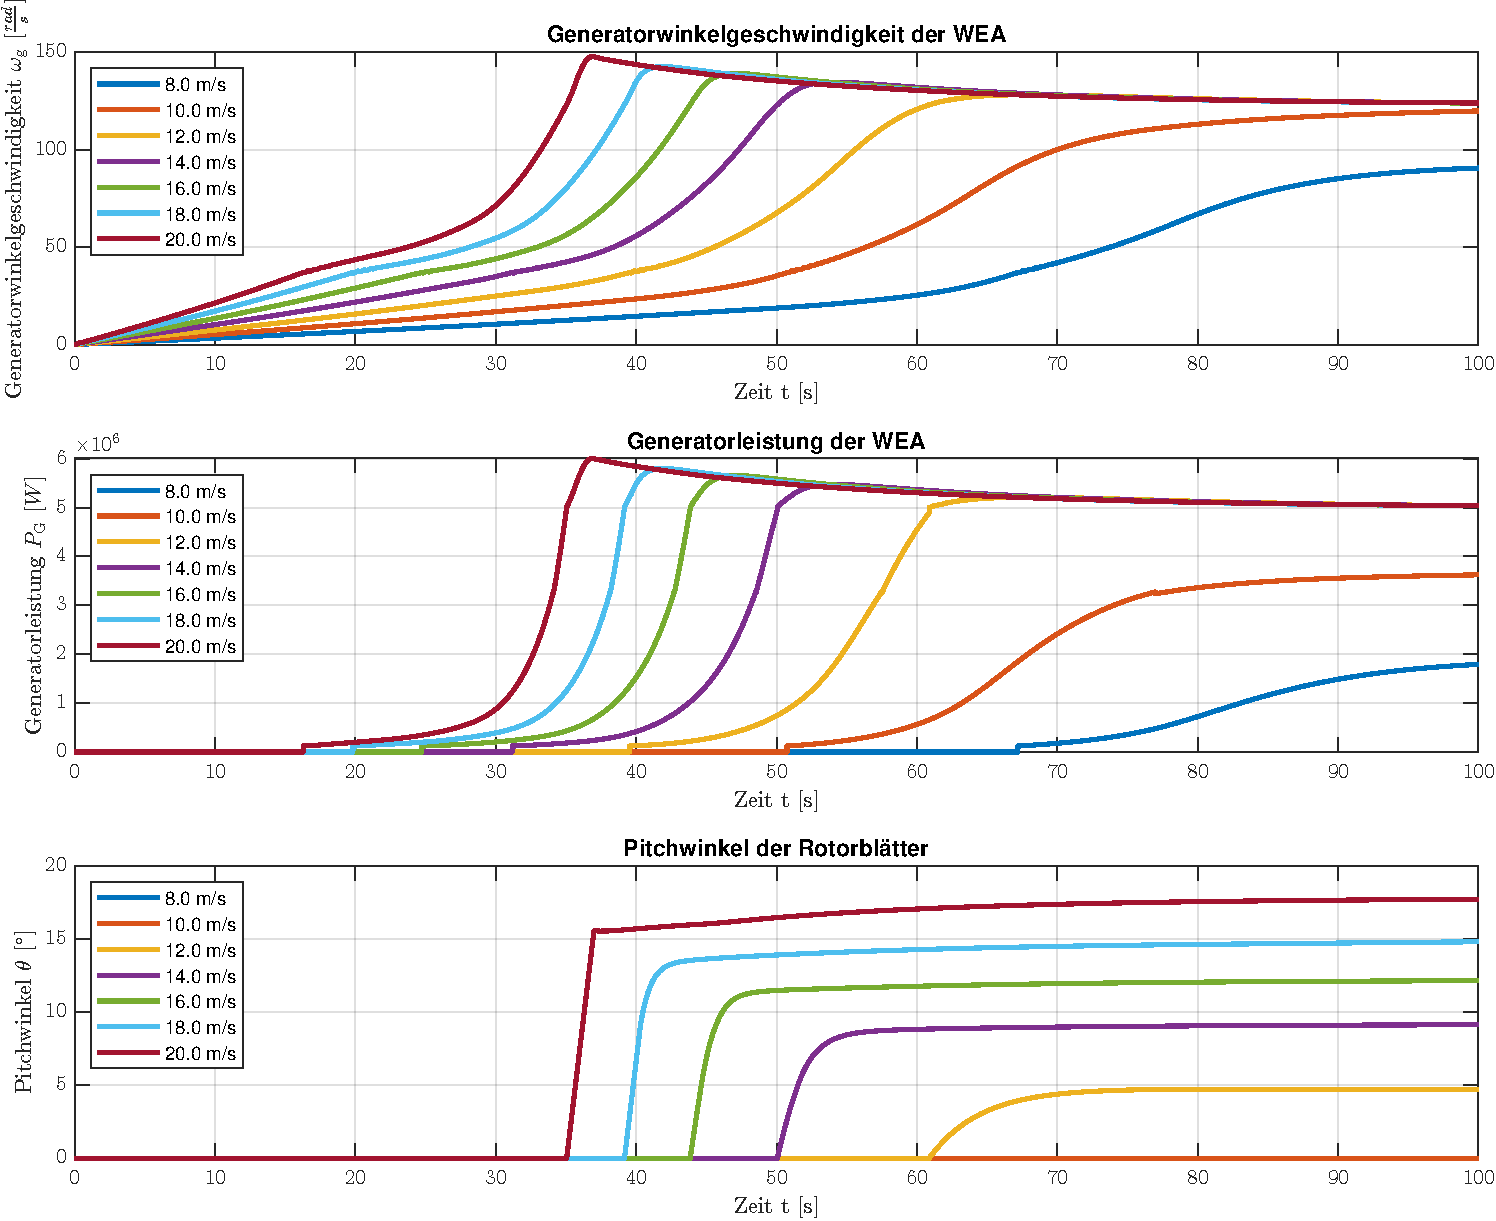
\includegraphics[width=1\textwidth]{Bilder/Kapitel 6/Reglervalidierung/const_wind_vgl.pdf}}
   \caption[Vergleich bei Verschiedenen Windgeschwindigkeiten]{Vergleich der Simulationsergebnisse bei verschiedenen konstanten Windgeschwindigkeiten zwischen $\SI{8}{\frac{m}{s}}$ bis $\SI{20}{\frac{m}{s}}$}
   \label{fig:Bild4.10}
\end{figure}

Es fällt weiterhin auf, dass bei $v_1 = \SI{8}{\frac{m}{s}}$ nicht die Nenndrehzahl als Endwert erreicht wird. Grund dafür ist, dass bei dieser recht kleinen Windgeschwindigkeit der obere Teillastbereich nicht erreicht wird und somit die Drehzahl nicht auf die Nenndrehzahl geregelt wird. Ebenfalls zu erkennen ist, dass je stärker der Wind ist, desto größer das Überschwingen der Drehzahl ist. Dies ist zu begründen über die Größe des benötigten Pitchwinkels, um die Drehzahl konstant zu halten. Umso größer der benötigte Pitchwinkel, desto größer das Überschwingen. Nach Abschluss des Ausgleichvorgangs wird jedoch für alle Windgeschwindigkeiten, die Drehzahlen für mindestens den oberen Teillastbereich erreichen, die Generatordrehzahl gleich der Nenndrehzahl.\\
Auch im mittleren Bereich der Abbildung sind gleiche Zusammenhänge für die Generatorleistung zu erkennen. Wesentlicher Unterschied zu der Drehzahldarstellung ist, dass erst ab dem Erreichen des unteren Teillastbereiches eine Leistung ausgegeben wird. Der Zeitpunkt dafür wird bei steigender Windgeschwindigkeit immer früher erreicht. Die Nennleistung kann bei allen Winden bis auf $v_1 = \SI{8}{\frac{m}{s}}$ und $v_1 = \SI{10}{\frac{m}{s}}$ hergestellt werden. Die beiden erwähnten Windgeschwindigkeiten reichen nicht aus, um eine ausreichend große Drehzahl für den Volllastbereich zu generieren. Erst im Volllastbereich wird auf die Nennleistung geregelt.\\
Im untersten Abschnitt der Grafik wird der Pitchwinkel gezeigt. Da das Pitchen erst ab dem Volllastbereich einsetzt, bleiben die Pitchwinkel für $v_1 = \SI{8}{\frac{m}{s}}$ und $v_1 = \SI{10}{\frac{m}{s}}$ dauerhaft bei $0^\circ$. Das Eintreten des Volllastbereiches bestimmt den Zeitpunkt des Pitch-Beginns. Mit steigender Windgeschwindigkeit verringert sich die Zeit bis zum Beginn der Pitch-Regelung.\\

% ---------------------------------

Als nächster Windtyp werden Windböen getestet. Es tritt genau eine Böe bei einer ansonsten konstanten Windgeschwindigkeit auf. Es soll gezeigt werden, welchen Einfluss eine einzelne starke Änderung des Windes auf die Regelung hat. Es werden an dieser Stelle zwei unterschiedlich große Böen auf das Modell eingeprägt.\\
\autoref{fig:Bild4.11} zeigt zunächst die Simulationsergebnisse für einen Wind mit $v_1 = \SI{8}{\frac{m}{s}}$ mit einer Böenamplitude von \ca $\SI{11.5}{\frac{m}{s}}$. Im Vergleich zu \autoref{fig:Bild4.7} sind kaum Unterschiede zu erkennen, was als positiv zu bewerten ist. Lediglich der Zeitpunkt des Eintritts des unteren Teillastbereiches wird um ein bis zwei Sekunden verringert und die Endwerte für Generatorleistung, -winkelgeschwindigkeit und -moment werden minimal größer.

\begin{figure}[H]
   \centering
   \fbox{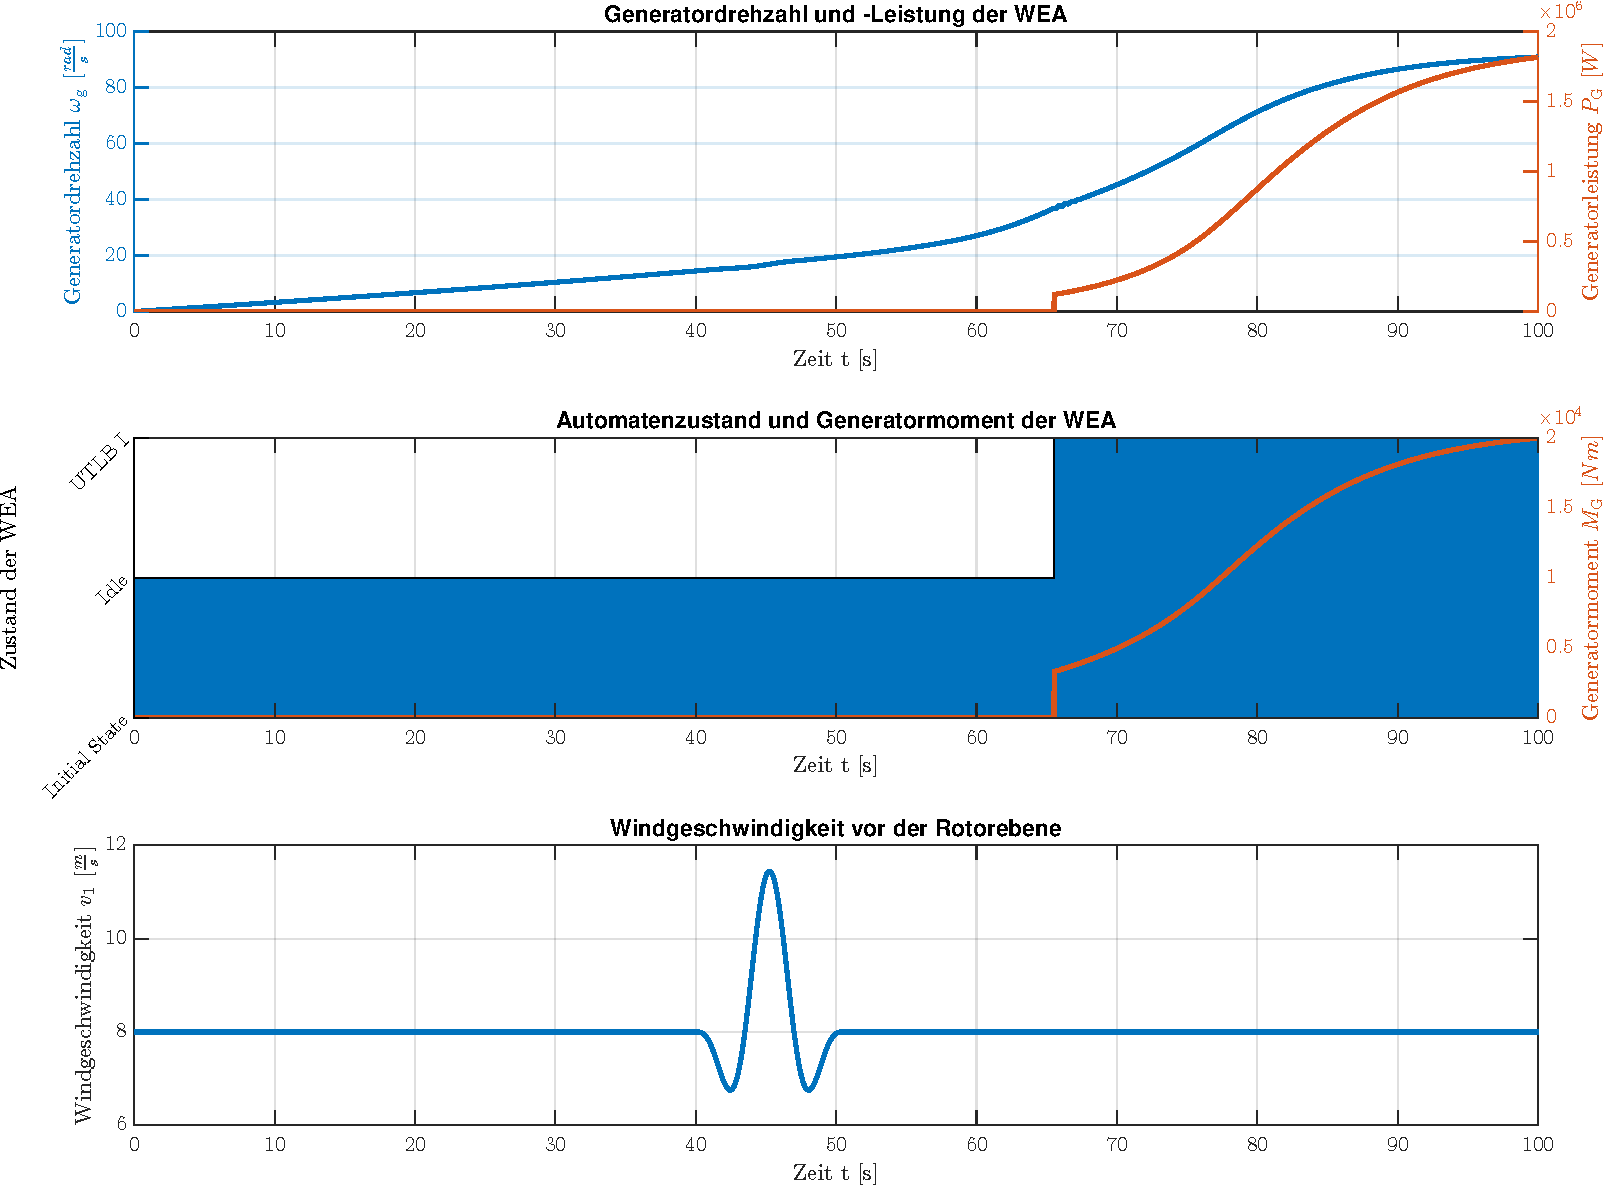
\includegraphics[width=1\textwidth]{Bilder/Kapitel 6/Reglervalidierung/gust_low.pdf}}
   \caption[Windböensimulation bei langsamem Wind]{Simulationsergebnisse für einen konstanten Wind mit $v_1 = \SI{8}{\frac{m}{s}}$ und einer Windböe mit einer Amplitude bei $\SI{11.5}{\frac{m}{s}}$}
   \label{fig:Bild4.11}
\end{figure}

Bei \autoref{fig:Bild4.12} ist im Gegensatz zur vorangegangenen Grafik kein Unterschied in den stationären Endwerten im Vergleich zu \autoref{fig:Bild4.9} zu erkennen. Zu begründen ist dies durch den Regler des Volllastbereiches, der zum Ziel hat, das Moment und die Drehzahl konstant zu halten. Da das Auftreten der Böe im unteren und oberen Teillastbereich stattfindet, werden jedoch sowohl die Drehzahl, als auch das Moment und die Leistung beeinflusst. Durch den lokalen Anstieg der Windgeschwindigkeit beschleunigt der Rotor leicht, was zu einer Vergrößerung der Generatordrehzahl führt. Da die Drehzahl steigt, sinkt die Steigung des Momentes und der dazu proportionalen Leistung kurzzeitig ab.

\begin{figure}[H]
   \centering
   \fbox{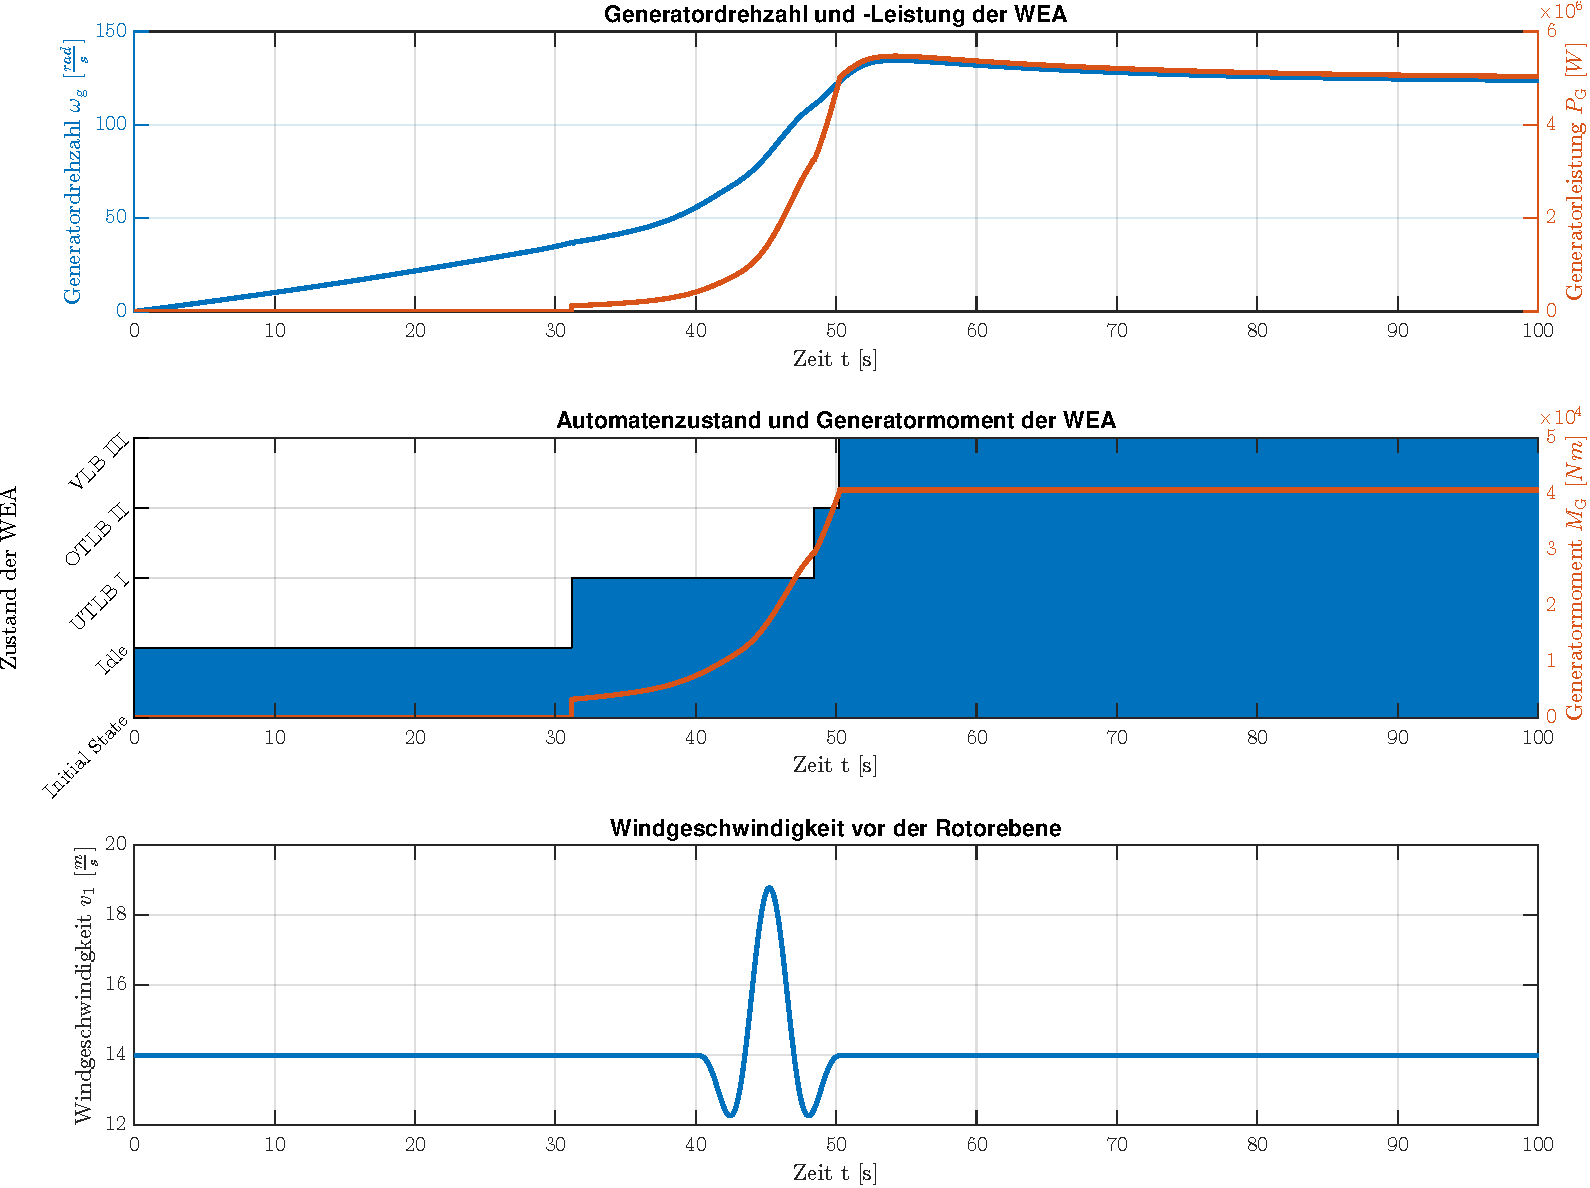
\includegraphics[width=1\textwidth]{Bilder/Kapitel 6/Reglervalidierung/gust_high.pdf}}
   \caption[Windböensimulation bei schnellem Wind]{Simulationsergebnisse für einen konstanten Wind mit $v_1 = \SI{14}{\frac{m}{s}}$ und einer Windböe mit einer Amplitude bei $\SI{19}{\frac{m}{s}}$}
   \label{fig:Bild4.12}
\end{figure}

% ---------------------------------

Im Folgenden soll das WEA-Modell inklusive der Regelstruktur gegen turbulente Winde getestet werden. Die getesteten Windreihen kommen realen Winden sehr nah. Somit kann über die Bewertung der nachfolgenden drei Abbildungen eine Aussage über die Anwendbarkeit der entworfenen Regler in der Realität getroffen werden. Interessant bei der Untersuchung ist vor allem das Verhalten bei dem Überschreiten der kritischen Windgeschwindigkeit \acs{vkrit}. Ebenfalls validiert werden soll die Fähigkeit des Pitchreglers, das Generatormoment und die Generatordrehzahl im Volllastbereich möglichst konstant zu halten.\\
\autoref{fig:Bild4.13} zeigt die Simulationsergebnisse bei einer Belastung des Modells mit einem turbulenten Wind mit $v_1 = \SI{8}{\frac{m}{s}}$ im Mittel. Im Vergleich zu der Abbildung bei konstantem Wind (\autoref{fig:Bild4.7}) fallen nur im hinteren Bereich ab \ca $\SI{85}{s}$ signifikante Unterschiede in den Kurvenverläufen auf. Zunächst beschleunigt der Antriebsstrang, bis die maximale Drehzahl und das maximale Drehmoment bei gegebenem Wind erreicht sind. Durch die turbulenten Schwankungen im Wind und der Leistungsoptimierung im unteren Teillastbereich (\vgl \autoref{tab:Tabelle4.1}) schwanken die Drehzahl, das Moment und die Leistung des Rotors proportional zum Wind mit. 

\begin{figure}[H]
   \centering
   \fbox{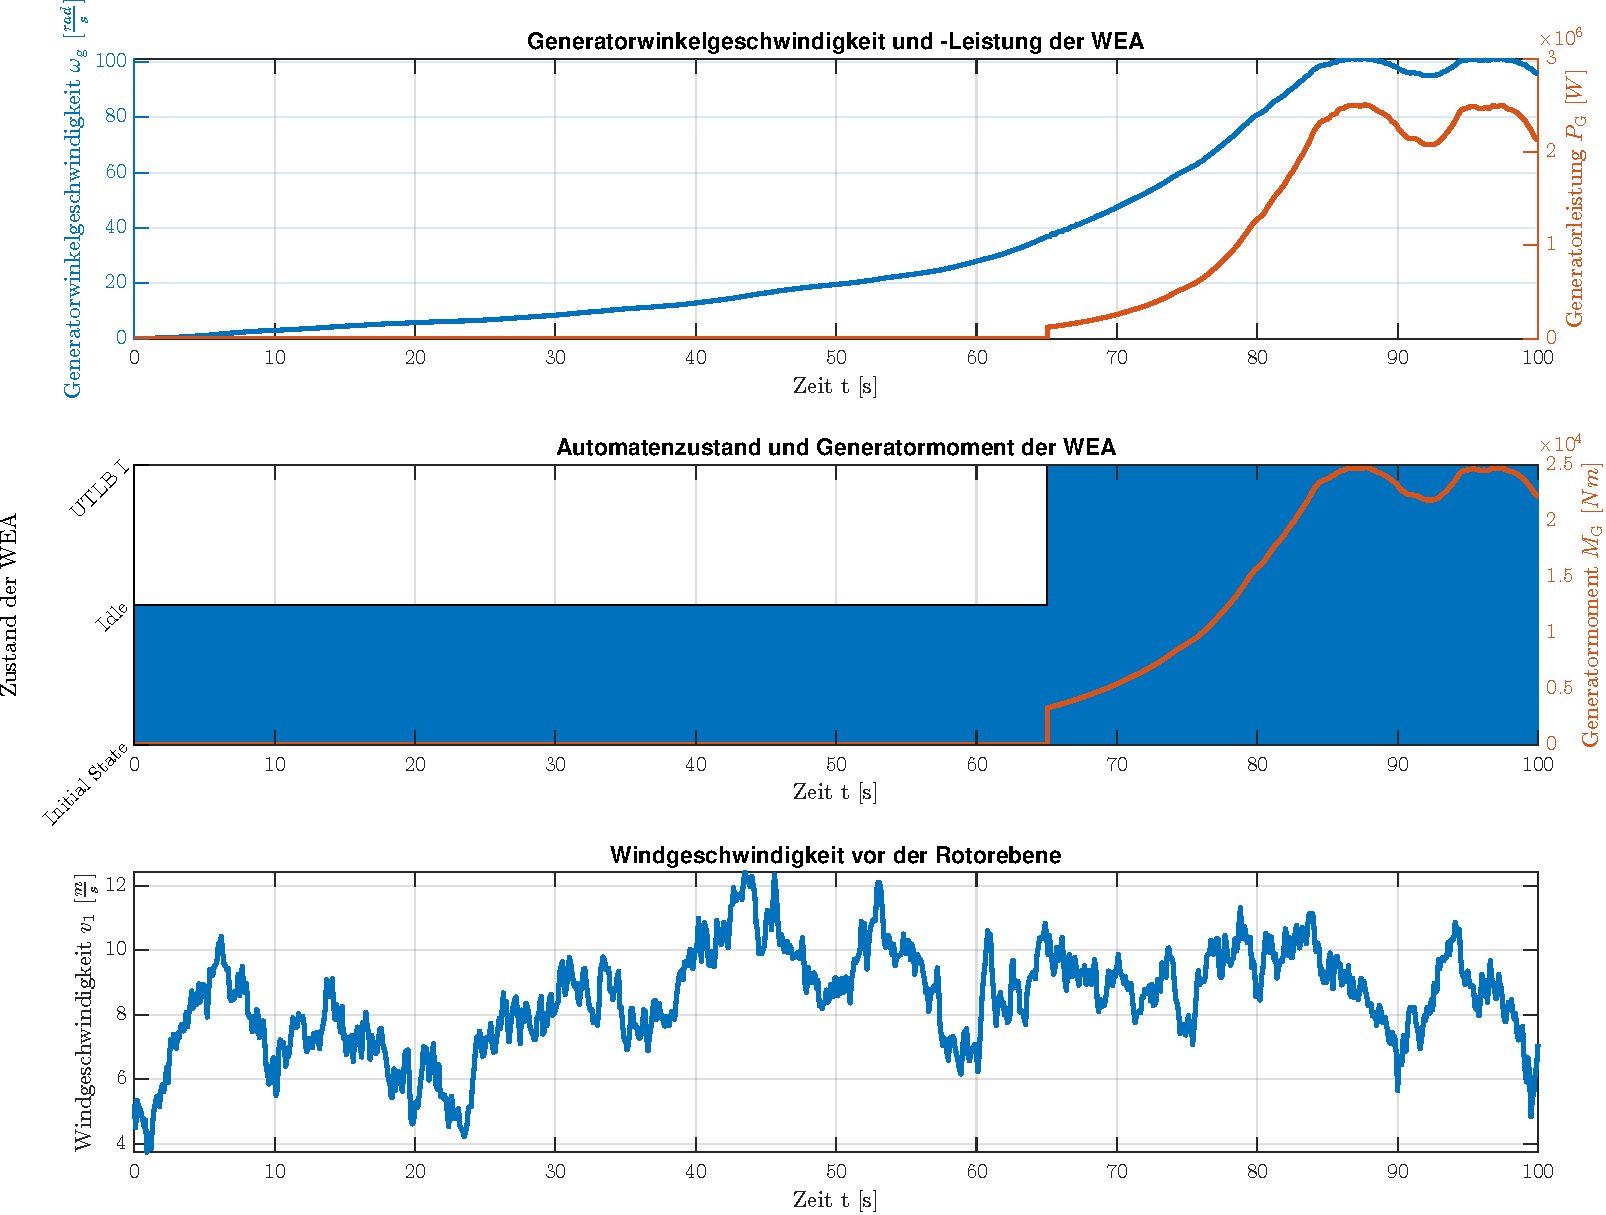
\includegraphics[width=1\textwidth]{Bilder/Kapitel 6/Reglervalidierung/turb_low.pdf}}
   \caption[Simulationsergebnisse bei langsamen turbulenten Winden]{Simulationsergebnisse bei turbulenten Winden mit einer mittleren Windgeschwindigkeit von $\SI{8}{\frac{m}{s}}$}
   \label{fig:Bild4.13}
\end{figure}

In \autoref{fig:Bild4.14} ist ein ausreichend starker Wind dargestellt, so dass der Vollastbereich der Anlage erreicht wird. Gut zu erkennen ist im oberen Bereich der Abbildung, dass nach Abklingen des Überschwingens im Vollastbereich die Leistung und die Drehzahl annähernd konstant im Nennwert gehalten werden. Somit ist festzustellen, dass die Regelung des Pitchwinkels funktional ist. Besonders gut ist dies im untersten Teil der Grafik zu erkennen. Es fällt auf, dass der Pitchwinkel proportional zur Windgeschwindigkeit Änderungen erfährt. Lediglich ein kleines Delay ist auszumachen, welches aufgrund der Stellgrößenbegrenzung des Pitchmotors auf maximal $8^\circ$/s auftritt. Ebenfalls Grund dafür ist ein leicht dämpfendes Verhalten des Pitchreglers, welches aus der Berechnung der Reglerkoeffizienten hervorgeht. Genau diese Eigenschaften sorgen dafür, dass die Generatorleistung und die Generatordrehzahl nicht exakt auf dem Nennwert verweilen.

\begin{figure}[H]
   \centering
   \fbox{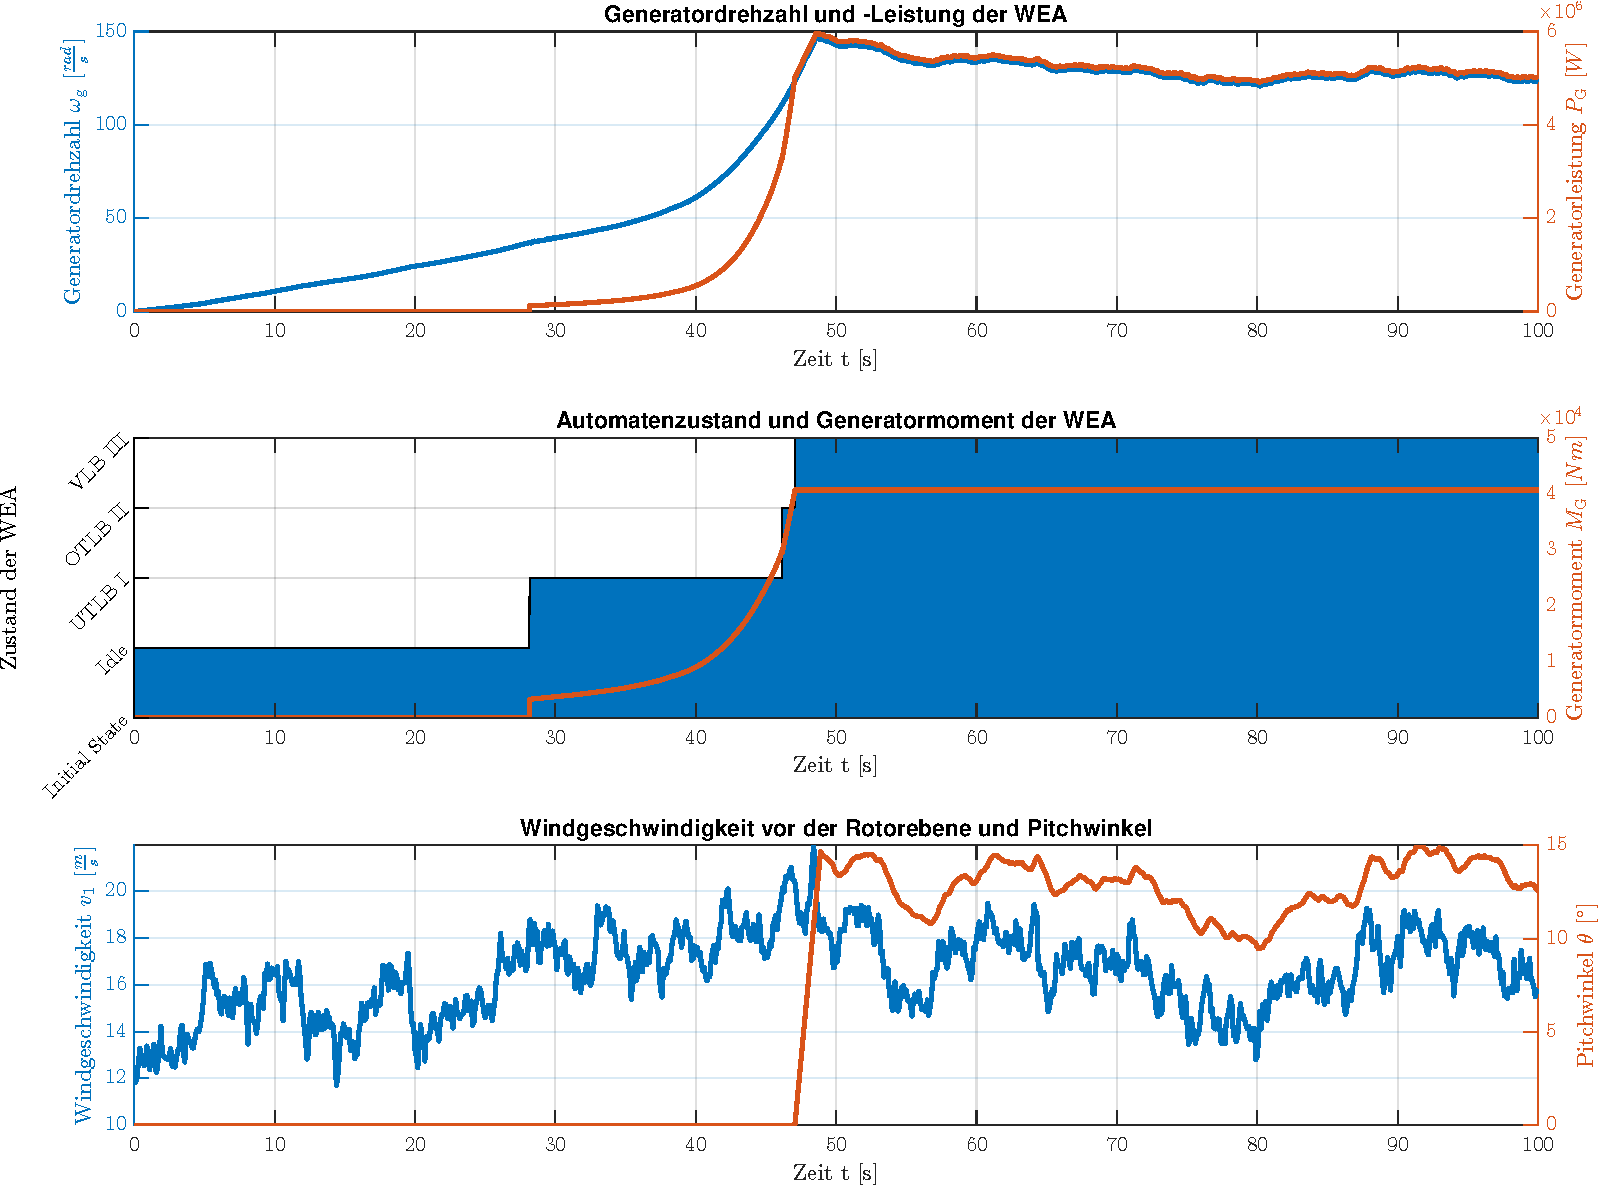
\includegraphics[width=1\textwidth]{Bilder/Kapitel 6/Reglervalidierung/turb_medium.pdf}}
   \caption[Simulationsergebnisse bei moderaten turbulenten Winden]{Simulationsergebnisse bei turbulenten Winden mit einer mittleren Windgeschwindigkeit von $\SI{16}{\frac{m}{s}}$}
   \label{fig:Bild4.14}
\end{figure}

Bei \autoref{fig:Bild4.15} soll das Verhalten der Anlage bei turbulenten Winden geprüft werden, welche die kritische Windgeschwindigkeit $\acs{vkrit} = \SI{25}{\frac{m}{s}}$ überschreiten. Die Kurvenverläufe in den ersten $\SI{75}{s}$ verhalten sich analog zu denen in \autoref{fig:Bild4.14}. Anschließend wird mehrmals kurzzeitig die maximale Schwelle überschritten, was gut am Verlauf des Windes im unteren Bereich von \autoref{fig:Bild4.15} zu sehen ist. Im mittleren Teil der Grafik ist zu erkennen, dass die Anlage in den E-Stop-Zustand (Nothalt) umschaltet. Erst nach unterschreiten von $90\%$ der kritischen Windgeschwindigkeit (\vgl \autoref{fig:Abbildung4.6} Zustand E-Stop) geht die WEA wieder zurück in den Idle-Zustand und läuft nachfolgend wieder an. Da der Wind im Fall der gezeigten Simulationsergebnisse nach kurzer Zeit wieder die kritische Windgeschwindigkeit überschreitet, geht die Anlage erneut in den Stop-Zustand. Das schnelle Wechseln der Zustände ist möglicherweise als nicht optimal anzusehen und bedarf einer Optimierung. Einen Vorschlag dafür liefert der \autoref{ausblick} \texttt{Ausblick}.  

\begin{figure}[H]
   \centering
   \fbox{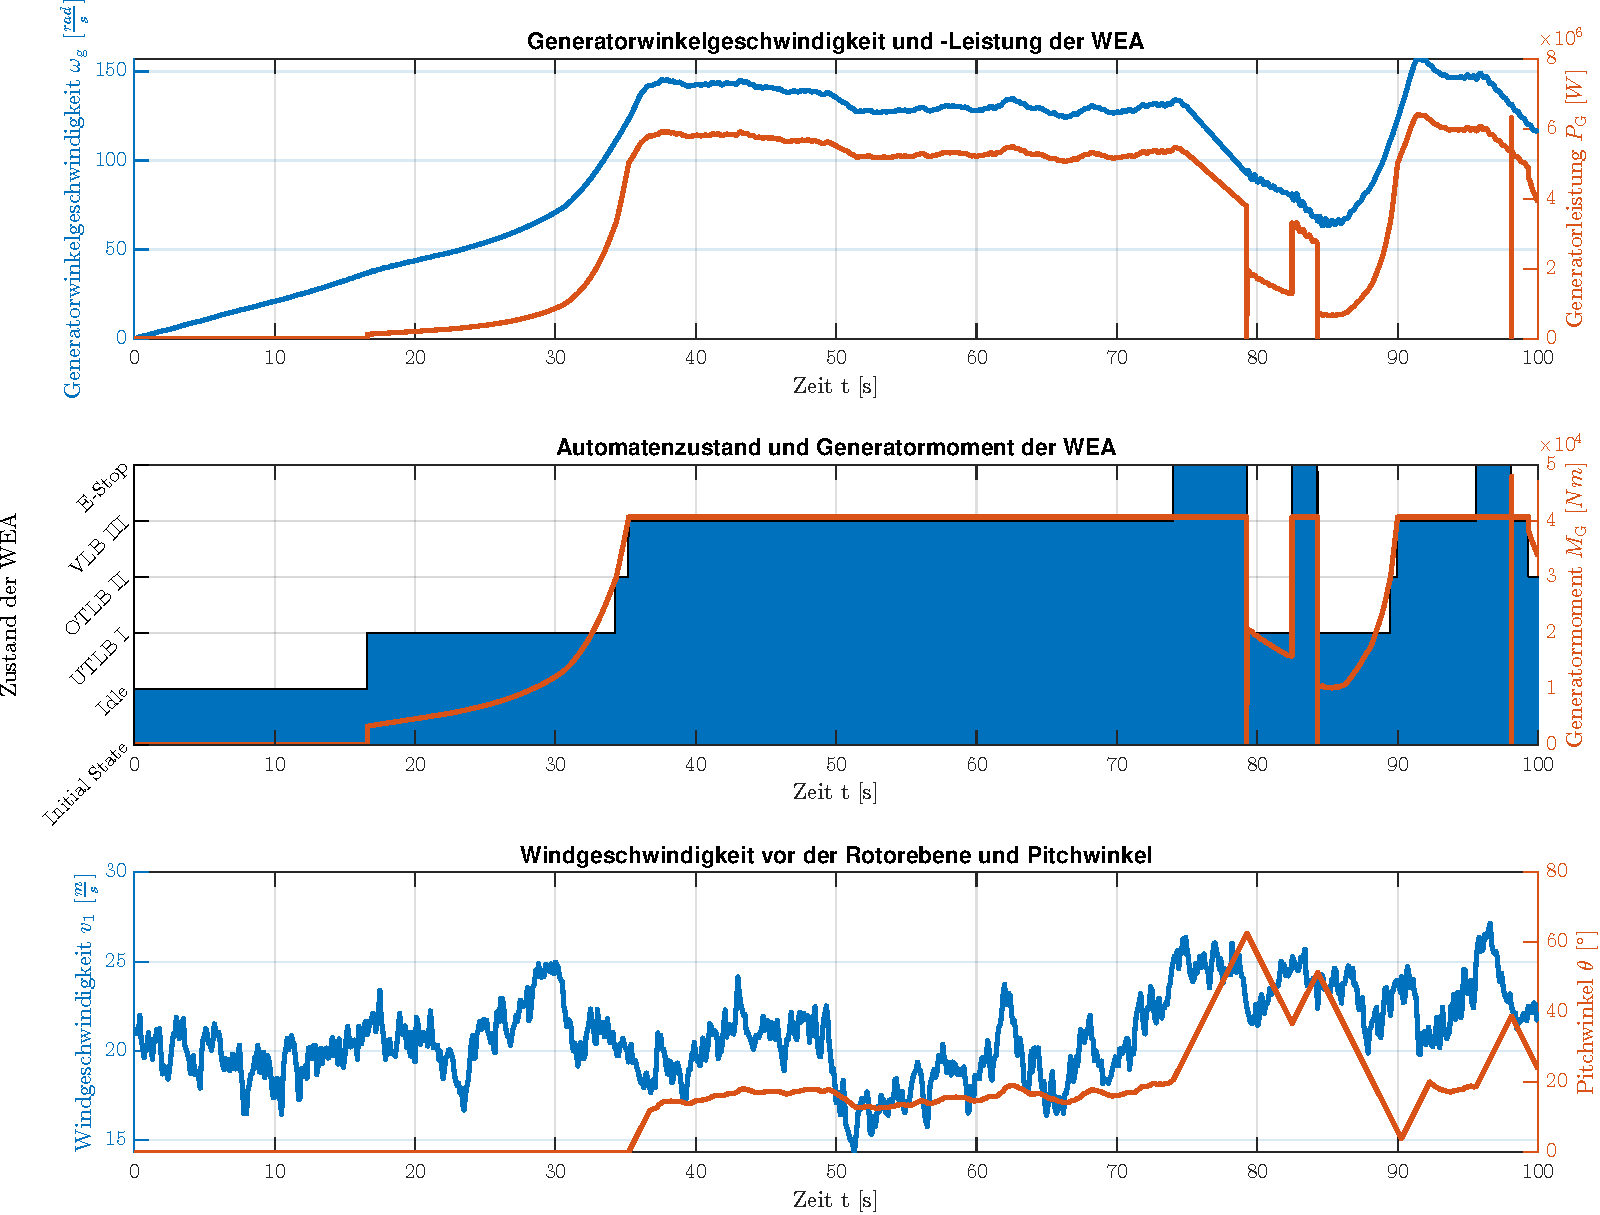
\includegraphics[width=1\textwidth]{Bilder/Kapitel 6/Reglervalidierung/turb_high.pdf}}
   \caption[Simulationsergebnisse bei schnellen turbulenten Winden]{Simulationsergebnisse bei turbulenten Winden mit einer mittleren Windgeschwindigkeit von $\SI{20}{\frac{m}{s}}$}
   \label{fig:Bild4.15}
\end{figure}

% ---------------------------------

Zuletzt wird eine Analyse der Ergebnisse der Simulation von Modell und Reglern gegen einen stufenförmigen Wind vorgenommen. Ziel ist es insbesondere das transiente Verhalten der Regler zu untersuchen, welches als besonders kritisch bei der maximalen Belastung des Modells durch unendlich steile Flanken im Wind einzustufen sind. Weiterhin ist der Wind in seiner letzten Stufe so gewählt, dass die Anlage bei maximaler Auslastung durch einen Wind von $v_1 = \SI{25}{\frac{m}{s}}$ betrieben wird.\\
\autoref{fig:Bild4.16} zeigt die Ergebnisse der Simulation. Beim der Betrachtung des obersten und untersten Bildausschnitts ist klar zu erkennen, dass der Sprung auf die maximale Windgeschwindigkeit für eine ruckartige Erhöhung der Beschleunigung des Rotors sorgt, was gut an der Generatorwinkelgeschwindigkeit auszumachen ist. Da die Windgeschwindigkeit und die Rotordrehzahl zu Beginn des Volllastbereiches sehr groß sind, kommt es auf Grund des initialen Pitchwinkels von $0^\circ$ zu einer starken Vergrößerung der \ac{FS}. Diese wiederum sorgt für eine Überhöhung der Generatorleistung über den Nennwert hinaus. Somit steigt der Pitchwinkel mit seiner maximalen Winkelgeschwindigkeit an, bis der benötigte Winkel erreicht ist. Da die Schubkraft durch die Vergrößerung des Pitchwinkels schnell wieder abfällt und somit auch die Leistung wieder zurückfällt, nimmt auch der Pitchwinkel wieder ab, bis sich alle Kurven zum Ende der Abbildung in einen stationären Endwert einfinden.

\begin{figure}[H]
   \centering
   \fbox{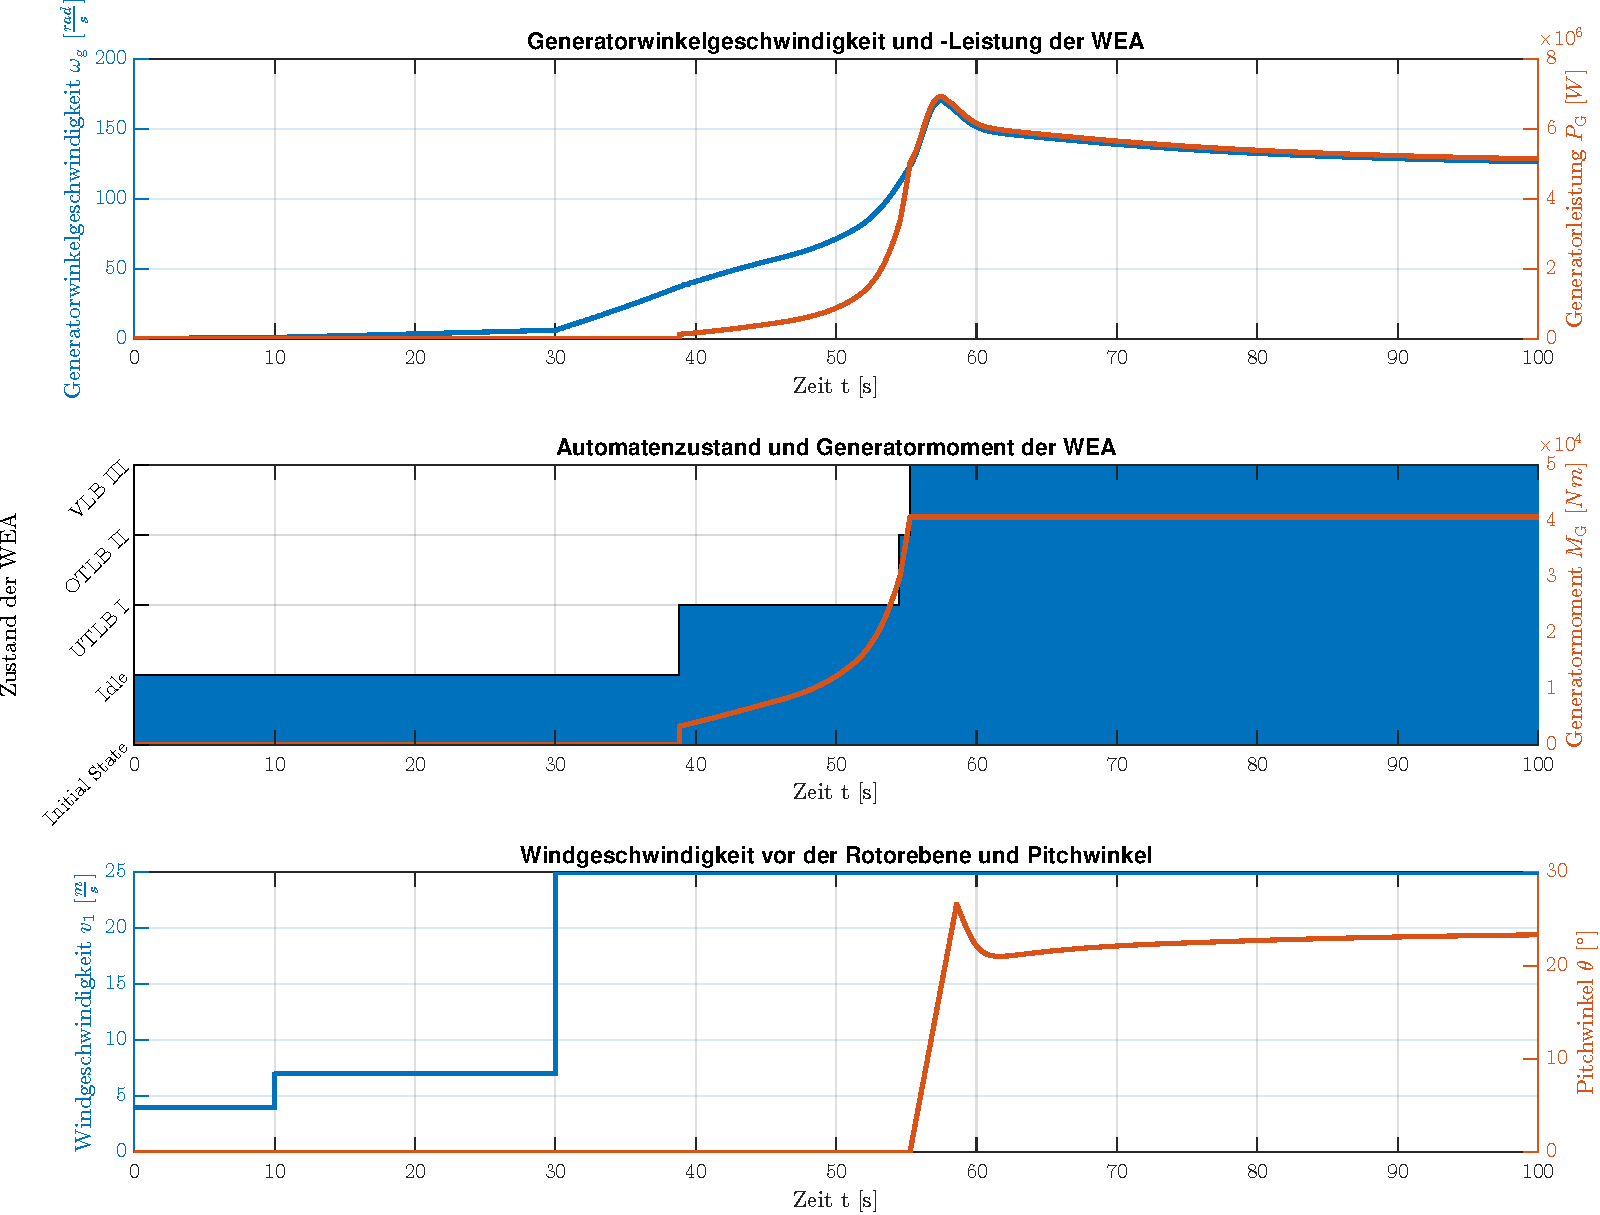
\includegraphics[width=1\textwidth]{Bilder/Kapitel 6/Reglervalidierung/wind_steps.pdf}}
   \caption[Simulationsergebnisse bei stufenförmigem Wind]{Simulationsergebnisse für einen eingeprägten stufenförmigem Wind bei einer maximalen Windgeschwindigkeit von $\SI{25}{\frac{m}{s}}$}
   \label{fig:Bild4.16}
\end{figure}

\subsubsection{Validierung der Regelziele}

Wie bereits in \autoref{regelziel} postuliert wurde, ist die Regelung in drei Arbeitsbereiche eingeteilt worden. Im unteren und oberen Teillastbereich findet eine Leistungsoptimierung statt. Im Vollastbereich wird hingegen die Leistung begrenzt. Besagte Regelziele sollen an \autoref{fig:Bild4.17} und \autoref{fig:Bild4.18} aufgezeigt werden.\\

\begin{figure}[H]
   \centering
   \fbox{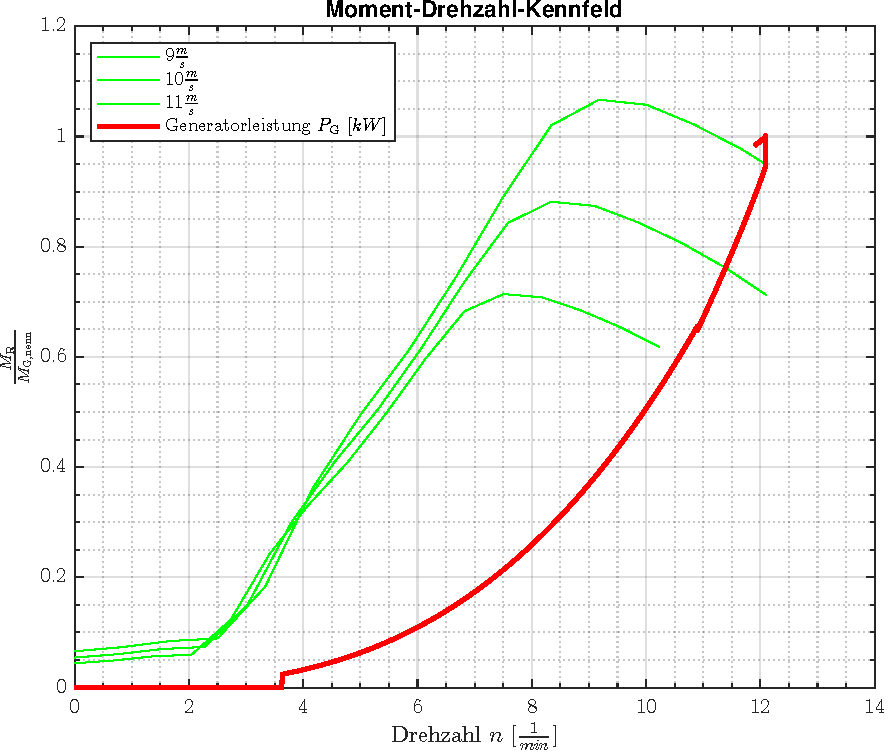
\includegraphics[width=0.95\textwidth]{Bilder/Kapitel 6/Reglervalidierung/moment_drehzahl_kennfeld.pdf}}
   \caption[Simulation des Moment-Drehzahl-Kennfelds]{Simulationsergebnisse für die Darstellung des Moment-Drehzahl-Kennfelds}
   \label{fig:Bild4.17}
\end{figure}
Zunächst wird der untere Teillastbereich betrachtet. Ziel war es die Drehzahl optimal an die Windgeschwindigkeit anzupassen, so dass sich ein optimales Anströmverhältnis ergibt. Das heißt, dass mit ansteigender Windgeschwindigkeit \acs{v1} stets das Leistungsmaximum aus der jeweiligen Windleistung entnommen wird (also $c_{\mathrm{P}} = c_{\mathrm{P,max}}$). \autoref{fig:Bild4.17} zeigt genau diesen Zusammenhang an der Kurve der Generatorleistung \acs{PG}. Wird die minimale Drehzahl ($30\%$ der Nenndrehzahl) überschritten, steigt das Rotormoment mit steigender Drehzahl.\\
Gut zu erkennen ist, dass ab $95\%$ der Nennleistung die Nenndrehzahl erreicht ist. Nun befindet sich die WEA im oberen Teillastbereich und lediglich das Drehmoment kann bis zum Nennmoment ansteigen. Der Bereich des oberen Teillastbereiches ist gut an dem senkrechten Verlauf der Generatorleistung zu erkennen.\\

\begin{figure}[H]
   \centering
   \fbox{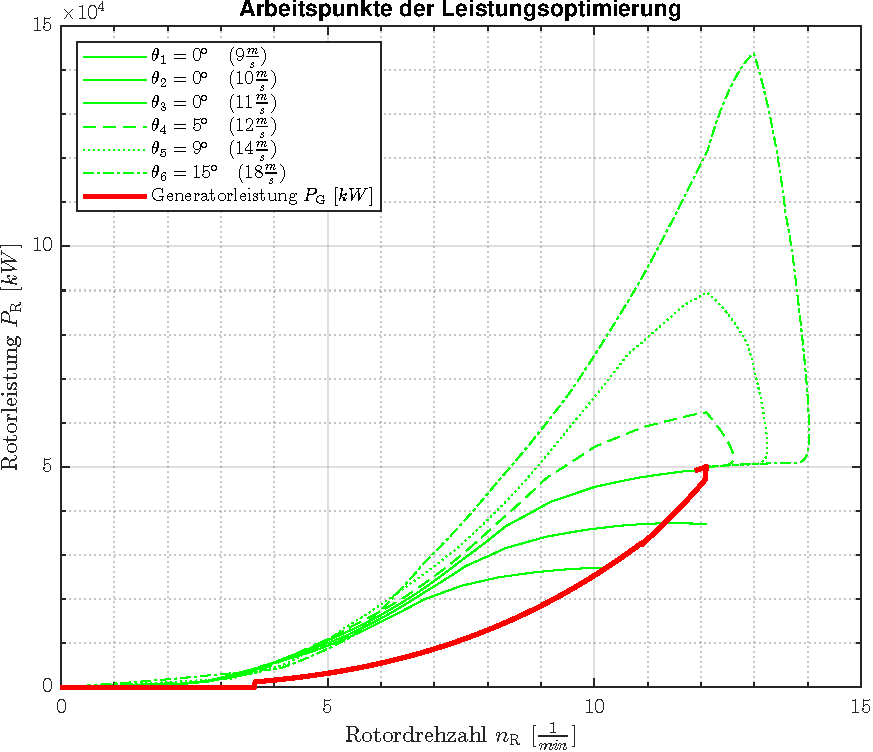
\includegraphics[width=0.95\textwidth]{Bilder/Kapitel 6/Reglervalidierung/valid_arbeitspunkte.pdf}}
   \caption[Simulation der Leistungsoptimierung]{Simulationsergebnisse für die Leistungsoptimierung zur Darstellung der Arbeitspunkte des Systems}
   \label{fig:Bild4.18}
\end{figure}

Ist das Nennmoment erreicht, bleiben sowohl Drehzahl als auch Moment konstant auf den Nennwerten. Der sich anschließende Bereich ist der Volllastbereich. Aus \autoref{fig:Bild4.18} geht hervor, dass bei größeren Winden nach erreichen der Nennwerte ein Pitchwinkel $>0^\circ$ eingestellt wird. Der Pitchwinkel steigt mit steigender Windgeschwindigkeit. Folglich wird die Leistung begrenzt.\\
Ebenfalls aus \autoref{fig:Bild4.18} abzulesen sind die Arbeitspunkte der Leistungsoptimierung. Es können die Verläufe aus \autoref{kennfelder} nachgebildet werden. Insbesondere \autoref{fig:Bild2.13} wird durch die Simulationsergebnisse bestätigt.

\subsubsection{Prüfung der Einhaltung der Constraints}

Ziel dieses Abschnittes ist zu Prüfen, inwiefern die gegebenen Begrenzungen des Systems in der Simulation eingehalten werden. Verifiziert werden muss insbesondere, inwieweit die Generatorleistung den geforderten Nennwert überschreitet, und ob es zu großen Auslenkungen der Rotorblätter und des Turmes kommt.\\
Begonnen wird zunächst mit der Validierung der Regler am Antriebsstrangmodell, welches in \autoref{modellierung_antriebsstrang} beschrieben ist. Zu erwarten ist, dass insbesondere hohe Windgeschwindigkeiten kritisch für die Einhaltung der Constraints sind.

\begin{figure}[H]
   \centering
   \fbox{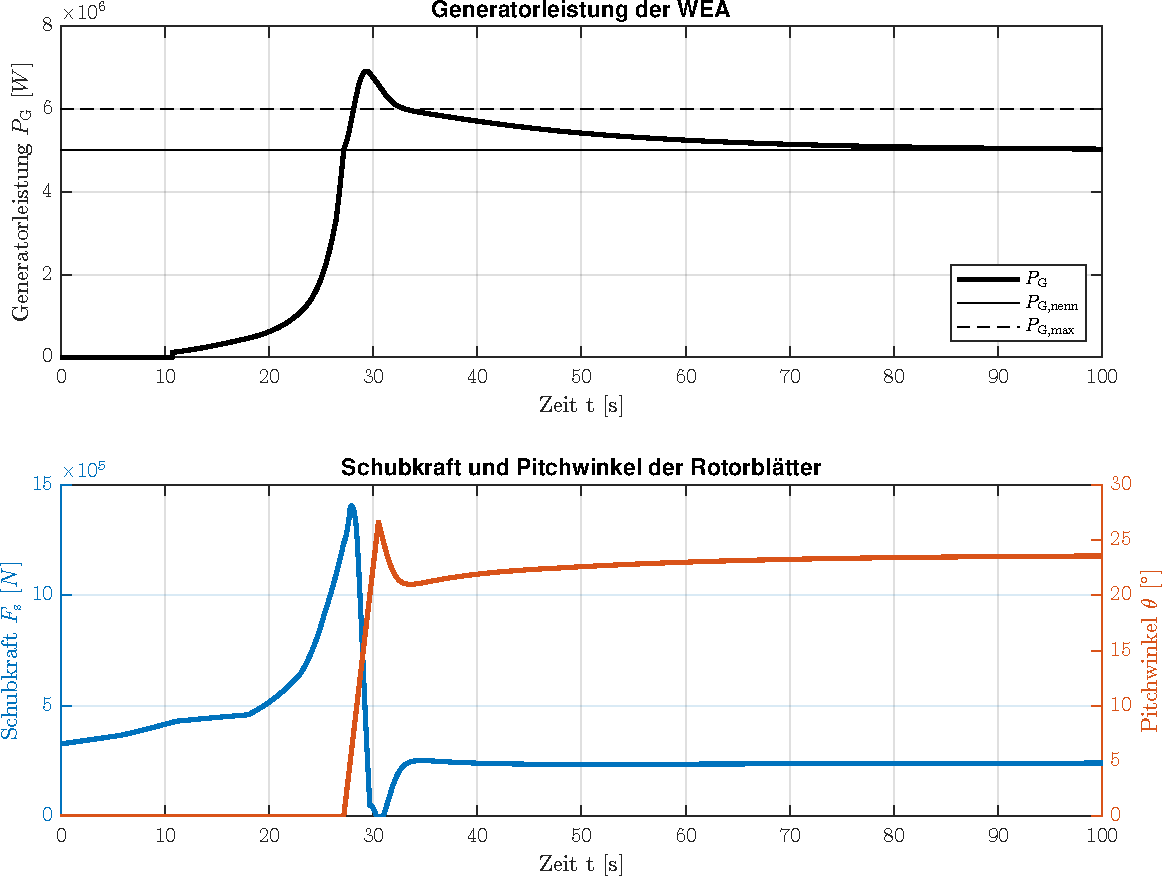
\includegraphics[width=0.85\textwidth]{Bilder/Kapitel 6/Reglervalidierung/constraint_leistung.pdf}}
   \caption[Constraint Leistungsbegrenzung]{Validierung der Leistungsbegrenzung bei $v_1 = \SI{25}{\frac{m}{s}}$}
   \label{fig:Bild4.19}
\end{figure}

\autoref{fig:Bild4.19} zeigt die Simulationsergebnisse zur Prüfung der Leistungsbegrenzung auf maximal 1.2-fache Nennleistung. Es kann festgehalten werden, dass bei sehr großen Windgeschwindigkeiten der Nennwert mehr als $20\%$ überschritten wird. Grund dafür zeigt sich in der unteren Hälfte der Grafik. Insbesondere im endenden unteren Teillastbereich und Volllastbereich steigt die Schubkraft stark an. Der Pitchvorgang beginnt jedoch erst mit $\acs{theta} = 0^\circ$ im Volllastbereich. Somit steigt die Rotordrehzahl weit über die Nenndrahzahl an, was wiederum auch zu einer übermäßig großen Steigerung der Leistung führt.\\

Weiterhin soll die implementierte Regelung und das Gesamtmodell für besonders kritische Winde auf die auftretenden Turm- und Blattauslenkungen untersucht werden. Die Eigenschaften dieses Teilmodells sind in \autoref{turm_blatt} beschrieben.\\

\begin{figure}[H]
   \centering
   \fbox{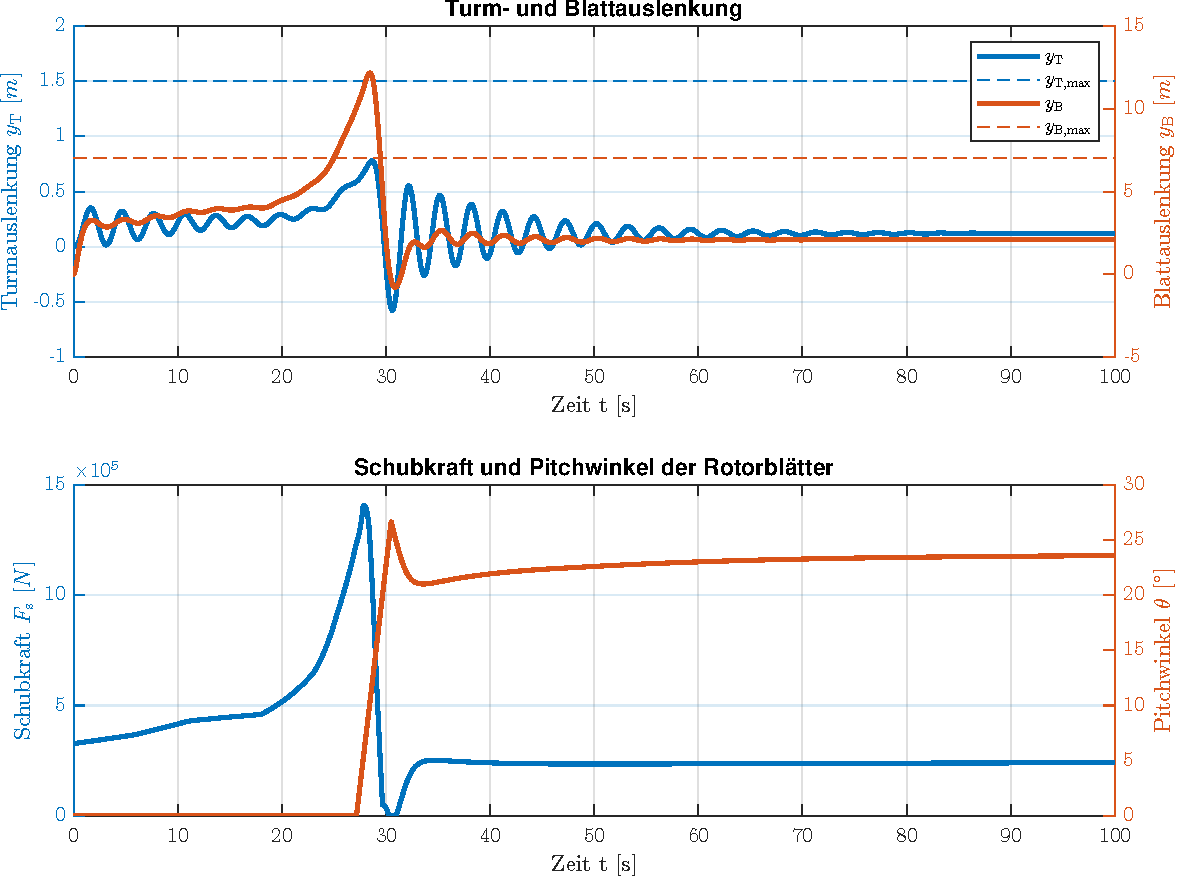
\includegraphics[width=1\textwidth]{Bilder/Kapitel 6/Reglervalidierung/constraint_auslenkung.pdf}}
   \caption[Constraint Turm- und Blattauslenkung]{Validierung der Turm- und Blattauslenkungen bei $v_1 = \SI{25}{\frac{m}{s}}$}
   \label{fig:Bild4.20}
\end{figure}

\autoref{fig:Bild4.20} zeigt die Simulationsergebnisse zur Prüfung der Begrenzung der Turm- und Blattauslenkungen auf maximal $\SI{1.5}{m}$ \bzw $\SI{7}{m}$. Die maximale Turmauslenkung wird nicht überschritten, was sich an den blauen Graphen im oberen Teil der Abbildung zeigt. Jedoch ist festzustellen, dass bei hohen Windgeschwindigkeiten zu große Blattauslenkungen auftreten. Die Begründung beruht auf dem gleichen Zusammenhang wie auch schon bei der Leistungsbegrenzung im vorangegangenen Bild. Die Schubkraft auf die Blätter steigt sehr stark an. Erst nach dem Einsetzen des Pitchvorgangs geht die Schubkraft und damit auch die Blattauslenkung wieder zurück. In der Grafik ist gut zu erkennen, dass die Hüllkurve der Auslenkung proportional zur Schubkraft ist. Sowohl die Rotorblätter als auch der Turm schwingen nach der Anregung stark.\\

Mögliche Lösungsansätze für das Einhalten der Constraints sind im Ausblick beschrieben.

%Chris
\section{Modellierung von Rotorblatt und Turm} \label{turm_blatt}

\subsection{Vorbetrachtung}
Die Modellierung der Rotorblätter (weiter als Blatt bezeichnet) und des Turms erfolgt analog zur Modellierung des Triebstranges. Als Grundlage für die Modellbildung dient das Feder-Masse-Dämpfer-System. Daraus soll die Bewegungs-DGL für die Blätter und des Turms abgeleitet werden. Allerdings wird hier für die Modellierung eine translatorische Bewegung betrachtet. Damit die reale Auslenkung der Blätter und des Turms modelliert wird, müssen hierzu mathematische Modelle formuliert werden, die die Dynamik des Systems in Abhängigkeit von äußeren Belastungen beschreiben. Genauer wird hier die Auslenkung infolge von außen angreifenden Kräften betrachtet. Die Verwendung eines mathematischen Ersatzmodells dient zur Vereinfachung und Überführung komplexer technischer Systeme. Dies macht das System beschreibbar und deterministisch. 
\\
Für die reale Auslenkung der Blätter und des Turms wird die Blattverbiegung als kollektiv in Windrichtung und die Turmverbiegung in Windrichtung betrachtet. Ähnlich wie beim Triebstrang haben die Systemgrößen wie Steifigkeit, Dämpfung und Masse ebenfalls eine entscheidende Rolle bei der Modellierung. Die \autoref{fig:Abbildung5.1} zeigt schematisch die Auslenkung von Blätter und Turm. Die Schubkraft \acs{FS} bewirkt dabei die Blatterverbiegung \acs{yB} und die Turmverbiegung \acs{yT}. Die Auslenkung hängt maßgeblich von der Steifigkeit und Dämpfung beider Systeme ab. Eine hohe Steifigkeit und Dämpfung führt zur einer geringeren Auslenkung und damit auch zu einem schnelleren Ausschwingen bei Belastung, während eine geringe Steifigkeit und Dämpfung zu einer höheren Auslenkung und langsameres Ausschwingen bei Belastung führt.
\begin{figure}[H]
    \centering
    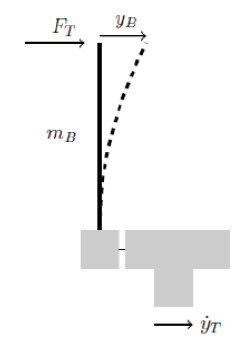
\includegraphics[scale=0.5]{Bilder/Kapitel 6/Auslenkung_Blatt.PNG}
    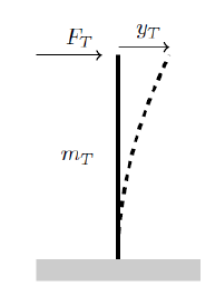
\includegraphics[scale=0.5]{Bilder/Kapitel 6/Auslenkung_Turm.PNG}
    \caption{Schematische Darstellung der Auslenkung der kollektiven Blätter \textit{(links)} und des Turms \textit{(rechts)}}
    \label{fig:Abbildung5.1}
\end{figure}
\newpage
Mit Hilfe der Bewegungs-DGL soll die reale Auslenkung der WEA beschrieben werden, damit zunächst abgeschätzt wird, ob eine Einhaltung der vorgegebenen Auslenkungsgrenzen vorliegt. Die WEA wird hierfür mit einer Bemessungswindgeschwindigkeit und einer daraus resultierenden Schubkraft \acs{FS} mechanisch von außen belastet. Das Modell wird als Funktionsblock in Matlab Simulink implementiert. 

\subsection{Feder-Masse-Dämpfer-System}
Als Grundlage für die Modellbildung dient das Feder-Masse-Dämpfer-System. Mithilfe dessen Vorüberlegungen und Ansätze wird das mathematische Modell für die Blätter und des Turms abgeleitet. Jeder mechanische Körper besitzt eine Steifigkeit \textit{k} und eine Dämpfung \textit{d}. Sofern eine Kraft \textit{F} auf den Körper wirkt, entsteht eine Auslenkung \textit{x}, welche von der Masse \textit{m} und den vorher besagten Größen abhängt. Die \autoref{fig:Abbildung5.2}{} zeigt den grundlegenden Aufbau eines solchen Systems.
Des Weiteren entsteht an jedem Element eine sogenannte Gegenkraft, welche der einwirkenden Kraft \textit{F} entgegenwirkt. Die Summe aller Kräfte innerhalb eines Systems ergibt sich zu 0, wodurch sich folgende Kräftebilanz in \autoref{eq:Gleichung 5.1} wiederfindet. Der Zusammenhang zwischen der Auslenkung \textit{x} und der Kraft \textit{F} kann als Differentialgleichung in \autoref{eq:Gleichung 5.2} beschrieben werden.
\begin{align}
    F(t) - F_{m}(t) - F_{k}(t) - F_{d}(t) = 0 
    \label{eq:Gleichung 5.1}
\end{align}

\begin{align}
    F(t) = m \cdot \frac{\delta^2x}{\delta^2t} + d \cdot \frac{\delta x}{\delta t} + k \cdot x(t)
    \label{eq:Gleichung 5.2}
\end{align}
\begin{figure}[H]
    \centering
    \scalebox{0.90}{
    \begin{tikzpicture}[framed,
        scale = 1.0,thick,>=triangle 45,
        spring/.style = {decorate,decoration={zigzag,amplitude=2pt,segment length=4pt}}
        ]
        
        %Raster
        %\draw [color=gray!10] [step=1mm] (-2.5cm,-0.5cm) grid (2.5cm,-5.5cm);
        %\draw [color=gray!30] [step=1cm] (-2.5cm,-0.5cm) grid (2.5cm,-5.5cm);

        %FederMasseDämpferSystem
	    \node[coordinate] (m) at (0.0,-2.0) {};
	    \node[draw,minimum size=1.5em] at (m) {$m$};
  	    \draw[shorten <=16pt] (m) -- coordinate (x) ++( 2,0);
  	    \draw[shorten <=16pt] (m) -- coordinate (f) ++(-2,0);
  	    \draw[<-] (f) -- node[left] {$F$} ++(0,-1);
        \draw[->] (x) -- node[right] {$x$} ++(0,1);
        \draw[shorten <=9.0pt] (m) -- +(0,-.7) coordinate (c);
        \draw (c) -| +( .7,-.3) coordinate (r);
        \draw (c) -| +(-.7,-.3) coordinate (l);
        \draw (r) -| +( .2,-1) node[right,pos=.75] {$d$};
        \draw (r) -| +(-.2,-1);
        \draw (r) +(-.15,-.5) -- coordinate (d) +(.15,-.5);
        \draw[spring] (l) -- node[left] {$k$} +(0,-1);
        \draw (l) ++(0,-1) -- ++(0,-.3) coordinate (b);
        \draw (d) |- (b);
        \draw (b -| m) -- ++(0,-.5) coordinate (g);
        \draw (g) +(-.5,0) -- +(.5,0);
        \foreach \i in {-1,0,1}
        \draw (g) ++(\i*.5,0) -- ++(225:.5);
 
    \end{tikzpicture}
    }
    \caption{Feder-Masse-Dämpfer-System}
    \label{fig:Abbildung5.2}
\end{figure}
\newpage
\subsection{Modellierung}

Für die Modellierung ist zu berücksichtigen, dass die Blätter und der Turm über die Gondel mechanisch miteinander gekoppelt sind. Ähnlich wie beim Triebstrang, bei dem die low speed shaft mit dem high speed shaft über das Getriebe und dessen Übersetzungsverhältnis gekoppelt ist. Das heißt, in den jeweiligen Bewegungs-DGL haben die Auslenkung der Blätter und des Turms einen gegenseitigen Einfluss aufeinander. Der einzige Unterschied der beiden Modellansätze ist, dass beim Triebstrang aufgrund einer rotatorischen Bewegung die Torsion der Wellen betrachtet wird, wobei sich ein Verschiebungswinkel $\varphi$ ergibt und bei der Modellierung der Blätter und des Turms sich durch die translatorische Bewegung eine Auslenkung \acs{yB} und \acs{yT} ergibt, wie in \autoref{fig:Abbildung5.3} dargestellt. Die Werte zur jeweiligen Masse, Steifigkeit und Dämpfung sind bereits gegeben. Da für die gesamte Modellierung der WEA eher die Auslenkung von Bedeutung ist, gilt es die \autoref{eq:Gleichung 5.2} so umzustellen, dass die benötigte Auslenkung der Blätter und des Turms berechnet wird. Eine zu große Auslenkung würde nämlich zur Zerstörung der WEA führen.
\\
Da für die Regelung der WEA lediglich ein vereinfachtes Funktionsmodell genutzt wird, werden dementsprechend die Auslenkungen nicht weiter regelungstechnisch berücksichtigt. Falls die Auslenkungen mit berücksichtigt werden sollen, müssen neue Regelziele formuliert werden, welche einen Einfluss auf das resultierende Referenzmodell für die Reglerauslegung hat. Damit ergäben sich auch neue Reglerkoeffizienten. Dennoch gilt es die definierten Grenzen einzuhalten und eine Bewertung über Blätter- und Turmauslenkung zu treffen.

\begin{figure}[H]
    \centering
    \scalebox{0.90}{
    \begin{tikzpicture}[framed,
        scale = 1.0,thick,>=triangle 45,
        spring/.style = {decorate,decoration={zigzag,amplitude=2pt,segment length=4pt}}
        ]
        
        %Raster
        %\draw [color=gray!10] [step=1mm] (-2.5cm,1.1cm) grid (2.5cm,-7.5cm);
        %\draw [color=gray!30] [step=1cm] (-2.5cm,1.1cm) grid (2.5cm,-7.5cm);

        %Blattmodell
        \node[draw,minimum size=1.5em] (mB) {$3\cdot m_B$};
        \draw[shorten <=3pt] (mB) -- coordinate (yB) ++( 2,0);
        \draw[shorten <=3pt] (mB) -- coordinate (f) ++(-2,0);
        \draw[<-] (f) -- node[left] {$F_S(t)$} ++(0,-1);
        \draw[->] (yB) -- node[right] {$y_B(t)$} ++(0,1);
        \draw (mB) -- +(0,-.7) coordinate (cB);
        \draw (cB) -| +( .7,-.3) coordinate (rB);
        \draw (cB) -| +(-.7,-.3) coordinate (lB);
        \draw (rB) -| +( .2,-1) node[right,pos=.75] {$3\cdot d_B$};
        \draw (rB) -| +(-.2,-1);
        \draw (rB) +(-.15,-.5) -- coordinate (dB) +(.15,-.5);
        \draw[spring] (lB) -- node[left] {$3\cdot k_B$} +(0,-1);
        \draw (lB) ++(0,-1) -- ++(0,-.3) coordinate (bB);
        \draw (dB) |- (bB);
        \draw (bB -| mB) -- ++(0,-.5) coordinate (gB);

        %Turmmodell
	    \node[coordinate] (mT) at (0.0,-4.0) {};
	    \draw[shorten <=9pt] (mT) -- (gB);
	    \node[draw,minimum size=1.5em] at (mT) {$m_T$};
  	    \draw[shorten <=16pt] (mT) -- coordinate (yT) ++( 2,0);
  	    \draw[shorten <=16pt] (mT) -- coordinate (f) ++(-2,0);
  	    \draw[<-] (f) -- node[left] {$F_S(t)$} ++(0,-1);
        \draw[->] (yT) -- node[right] {$y_T(t)$} ++(0,1);
        \draw[shorten <=9.0pt] (mT) -- +(0,-.7) coordinate (c);
        \draw (c) -| +( .7,-.3) coordinate (r);
        \draw (c) -| +(-.7,-.3) coordinate (l);
        \draw (r) -| +( .2,-1) node[right,pos=.75] {$d_T$};
        \draw (r) -| +(-.2,-1);
        \draw (r) +(-.15,-.5) -- coordinate (d) +(.15,-.5);
        \draw[spring] (l) -- node[left] {$k_T$} +(0,-1);
        \draw (l) ++(0,-1) -- ++(0,-.3) coordinate (b);
        \draw (d) |- (b);
        \draw (b -| mT) -- ++(0,-.5) coordinate (g);
        \draw (g) +(-.5,0) -- +(.5,0);
        \foreach \i in {-1,0,1}
        \draw (g) ++(\i*.5,0) -- ++(225:.5);
 
    \end{tikzpicture}
    }
    \caption{Feder-Masse-Dämpfer-System: Turm und Blätter}
    \label{fig:Abbildung5.3}
\end{figure}
\newpage
Die Auslenkung der kollektiven Blätter wirkt der Auslenkung des Turms entgegen, wodurch die Gegenkräfte der Steifigkeit und Dämpfung der Blätter mit einem positiven Vorzeichen in die Bewegungs-DGL mit einfließen. Die eigentliche Auslenkung ergibt sich aufgrund der mechanischen Kopplung aus der Differenz zwischen Blattverbiegung \acs{yB} und Turmverbiegung \acs{yT}. Die Steifigkeit und Dämpfung beziehen sich lediglich auf ein Blatt, wodurch diese Faktoren mit 3 multipliziert werden, um insgesamt das Verhalten der drei Blätter abzubilden.



Damit ergibt sich für die Bewegungs-DGL des Turms:

\begin{align}\label{eq:Gleichung 6.3}
    \boxed{\ddot{\acs{yT}}=\frac{-\acs{kT} \cdot \acs{yT}- \acs{dT} \cdot \dot{\acs{yT}}+ 3 \cdot \acs{kB} \cdot(\acs{yB}-\acs{yT})+ 3\cdot \acs{dB} \cdot (\dot{\acs{yB}}-\dot{\acs{yT}})+\acs{FS}} {\acs{mT}}}
\end{align}
\newline
Gleiches gilt für die effektiv schwingende Blattmasse \acs{mBla}. Aufgrund dessen verringert sich die Schubkraft \acs{FS} um ein Drittel. Für die Blätter ergibt sich folgende Bewegungs-DGL:

\begin{align}\label{eq:Gleichung6.4}
    \boxed{\ddot{\acs{yB}}=\frac{-3 \cdot \acs{kB} \cdot(\acs{yB}-\acs{yT})-3 \cdot \acs{dB} \cdot (\dot{\acs{yB}}-\dot{\acs{yT}})+\acs{FS}} {3\cdot\acs{mBla}}}
\end{align}

\subsection{Simulationsergebnisse}
Zu Beginn des Kapitels wurde bereits erwähnt, dass das Modell zu Blätter und Turm in einem Funktionsblock in Matlab Simulink implementiert wird. Zur vorläufigen Überprüfung des Modells wird vorerst das System mit einer konstanten Schubkraft \acs{FS} im Bemessungsbetrieb belastet. Dies soll zunächst eine Auskunft darüber geben, ob die resultierende Auslenkungen den Erwartungen entsprechen. Um eine genaue Aussage über das korrekte Gesamtverhalten des Modells zu treffen, muss das gesamte Modell mit Regelung betrachtet und getestet werden. 
Die Bemessungswindleistung der WEA beträgt:
\begin{align}
    \acs{v1} = 10 \frac {m}{s}
\end{align}
\\
Es wird ein Schubkraftbeiwert von \acs{cT} = 0,8 angenommen. Der Schubkraftbeiwert \acs{cT} sowie die daraus resultierende Schubkraft \acs{FS} ergeben sich später aus dem dimensionslosen Kennfeld der WEA. Mithilfe der \autoref{eq:Gleichung6.4} lässt sich nun eine Schubkraft \acs{FS} berechnen, die das System belastet. Die restlichen benötigten Größen sind Konstanten und bereits gegeben. Das Ergebnis ist der \autoref{eq:Gleichung 6.7} zu entnehmen. Die \autoref{fig:Abbildung5.4} zeigt die Ein- und Ausgangsparameter des Modells in Blockdarstellung für die Simulation.
\begin{align}
    \acs{FS} &= \frac{1}{2} \cdot \rho \cdot \pi \cdot \acs{R}^2 \cdot \acs{cT} \cdot \acs{v1}^2 \label{eq:Gleichung6.6} \\
    \acs{FS} &= \frac{1}{2} \cdot 1,225 \frac{kg}{m^3} \cdot \pi \cdot (63m)^2 \cdot 0,8 \cdot (10 \frac{m}{s})^2 \nonumber \\
    \acs{FS} &= \underline{\underline{610980,1 N}} \label{eq:Gleichung 6.7}
\end{align}

\begin{figure}[H]
   \centering
   \begin{pspicture}[showgrid=false](0,0)(10,5)
        \psframe(0,0)(10,5)
        % Eingänge
        \psline{->}(1,2.5)(3.5,2.5)
        \rput(1,2.9){\footnotesize \acs{FS}}

        % Modell
        \psframe[linecolor=black,fillcolor=lightGrey,fillstyle=solid](3.5,0.5)(6.5,4.5)
        \rput(5,2.8){\small Blatt- und}
        \rput(5,2.3){\small Turmmodell}
        % Ausgänge
        \psline{->}(6.5,3.0)(9,3.0)
        \rput(9,3.4){\footnotesize \acs{yT}}
        \psline{->}(6.5,2.0)(9,2.0)
        \rput(9,2.4){\footnotesize \acs{yB}}
    \end{pspicture}
   \caption[Blockdarstellung Turm- und Blattmodell]{Blockdarstellung des Blatt- und Turmmodells inklusive der Ein- und Ausgangsparameter}
   \label{fig:Abbildung5.4}
\end{figure}

Mit dem Ergebnis aus \autoref{eq:Gleichung 6.7} wird nun das Modell von außen mit einer konstanten Schubkraft \acs{FS} belastet. Die \autoref{fig:Abbildung5.5} zeigt die Auslenkungen von den kollektiven Blättern und des Turms. Aus der Simulation ist zu erkennen, dass die Auslenkung der Blätter deutlich höher im Vergleich zur Auslenkung des Turms ist. Dies begründet sich dadurch, dass der Turm eine deutlich größere Steifigkeit und Dämpfung aufweist. Zu Beginn der Belastung ist ein deutliches Schwingen beider Systeme zu erkennen. Nach einer gewissen Zeit erreichen Blätter und Turm einen stationären Endwert, wobei der Turm etwas früher einen stationären Endwert erreicht. Das Ausmaß der Auslenkung von Blätter und Turm wird in Bezug auf die vorgegebenen Grenzen so weit eingehalten. Jedoch muss dies im Gesamtmodell erneut verifiziert werden.
\\
Zusammenfassend lässt sich sagen, dass das Simulationsergebnis zu den Blättern und dem Turm den Erwartungen entspricht. Für eine genauere Aussage zur Richtigkeit der Modelle ist die Gesamtheit der Modellierung und dessen Ergebnis zu betrachten und neu zu beurteilen. Hier wurde lediglich die WEA mit dessen Bemessungswindleistung belastet. Im Realfall sind deutlich höhere Windgeschwindigkeiten durchaus denkbar. Des Weiteren geht die Windgeschwindigkeit quadratisch in die \autoref{eq:Gleichung6.6} mit ein, so dass die Schubkraft \acs{FS} ebenfalls quadratisch mit der Windgeschwindigkeit steigt und damit die WEA deutlich mehr belastet wird, was widerrum eine höhere Auslenkung beider Systeme zur Folge hat. Durch geeignete Pitchverstellung lässt sich jedoch die Belastung der WEA bei steigender Schubkraft \acs{FS} verringern, wodurch die erzeugte Energie zwar verringert wird, aber damit wird die WEA nicht durch zu hohe Belastungen zerstört. Hinzufügend sei zu erwähnen, dass eine Pitchverstellung lediglich indirekten Einfluss auf die Auslenkungen hat. Die Pitchverstellung dient zur Leistungsbegrenzung und nicht zur direkten Begrenzung von Auslenkungen.

 \begin{figure}[H]
    \centering
    \fbox{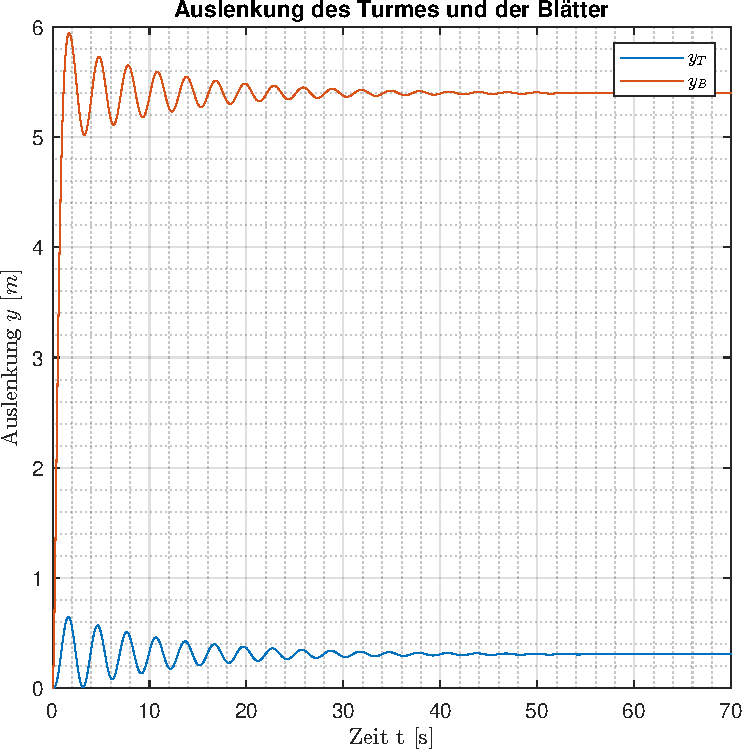
\includegraphics[width=0.9\textwidth]{Bilder/Kapitel 6/Auslenkungen.pdf}}
    \caption[Turm- und Blattauslenkung]{Auslenkung der kollektiven Blätter \textit{(orange)} und des Turmes \textit{(blau)}}
    \label{fig:Abbildung5.5}
\end{figure}

 %\underline{}
 
 %\underline{\underline{}}
 
 

% \section{Ausblick} \label{ausblick}

In dieser Ausarbeitung konnte erfolgreich gezeigt werden, wie eine Windenergieanlage modelliert und anschließend anhand des entwickelten Modells geregelt werden kann. Es hat sich jedoch auch gezeigt, dass einige Verbesserungen und Optimierungen von Nöten wären, bevor das Modell und insbesondere die Regelstruktur auf eine reale WEA angewendet werden kann. Nachfolgend sind die auffälligsten Mängel zusammengefasst mit möglichen Ansätzen für die Ausbesserung der Mängel \bzw die Optimierung des Verhaltens der Anlage.\\

Der Größte Mangel in der aktuellen Implementierung ist die Nichteinhaltung der gegebenen Constraints. Der Einsatz des implementierten Funktionsmodells würde voraussichtlich zur Zerstörung der realen Anlage sorgen. Als Lösungsansatz könnte der Detailgrad des Funktionsmodells angepasst werden, so dass als Grundlage für die Reglerimplementierung ein kombiniertes Rotor-/Turm-/Triebsstrangmodell dient.\\

Ebenfalls aufgefallen war das pendelnde Verhalten zwischen Betriebszuständen, wenn die maximale Windgeschwindigkeit in kurzen Zeitabständen überschritten wird. Hier wäre es vermutlich ratsam eine Zeitsperre in die Steuereinheit einzubauen, die dafür sorgt, dass die Anlage nicht sofort wieder anläuft. Es ist als wahrscheinlich einzustufen, dass wenn der Wind einmal die kritische Windgeschwindigkeit erreicht hat, dass er das auch weitere Male in der nächsten Zeit tut.\\

Die Reglervalidierung hat gezeigt, dass der obere Teillastbereich nur für einen sehr kleinen Bereich der Rotordrehzahl benötigt wird. Es ist schwer diesen Bereich dediziert anzufahren und damit auch nachzuweisen. Da der Bereich jedoch sehr klein ist, kann die Aussage getroffen werden, dass der vergleichsweise komplexe Regler auch mit einem Linearen Verhalten zwischen unterem- und Volllastbereich ersetzt werden könnte. Umgangssprachlich kann hier von einem over-Engineering geredet werden.\\

Als letzter Punkt soll an dieser Stelle noch die Relevanz eines Umrichters \bzw Umrichtermodells postuliert werden. Wie bereits in mehreren Stellen der Arbeit erwähnt, wurde lediglich das Störverhalten betrachtet. Die Implementierung eines Umrichters zur Leistungsoptimierung durch Drehzahlvariabilität würde die Umsetzung des Führungsverhaltens ermöglichen.

%---------Quellen---------------------------------
\newpage
\newcount\Quellennummer
\Quellennummer=1

\renewcommand\refname{Literaturverzeichnis}
\addcontentsline{toc}{section}{Literaturverzeichnis}

\begin{thebibliography}{999}
{\setlength{\emergencystretch}{3cm}%

\bibitem[\the\Quellennummer]{HTWgross}
HTW-Logo auf dem Deckblatt\par
\url{https://de.wikipedia.org/wiki/Datei:Logo_HTW_Berlin.svg} \par
 Stand: 17.08.2018 um 14:49 Uhr

\advance\Quellennummer by 1
 
\bibitem[\the\Quellennummer]{HTWklein}
HTW-Logo in der Kopfzeile\par
\url{http://tonkollektiv-htw.de/} \par
 Stand: 17.08.2018 um 14:53 Uhr

\advance\Quellennummer by 1

\bibitem[\the\Quellennummer]{SkriptSchulte}
Skript Automation in regenerativen Energiesystemen\par
Prof.\xspace Dr.\xspace -Ing.\xspace Horst Schulte

\advance\Quellennummer by 1

\bibitem[\the\Quellennummer]{LinBrandstaedter}
Anleitung Linearisierung eines zeitinvarianten,\par
nichtlinearen Zustandmodells\par
Prof.\xspace Dr.\xspace -Ing.\xspace Heide Brandstädter

\advance\Quellennummer by 1

\bibitem[\the\Quellennummer]{RegelungBuss}
Regelungs- und Steuerungstechnik: Polstellenverteilung\par
Prof.\xspace Dr.\xspace -Ing.\xspace M. Buss

\advance\Quellennummer by 1

}
\end{thebibliography}

\end{document}
